%\documentclass[preprint]{aastex}  % USE THIS TO MAKE BIB, THEN FORMAT USING EMULATEAPJ
\documentclass[twocolumn,numberedappendix]{emulateapj} \shorttitle{New Limits on the 21 cm Power Spectrum at $z=8.4$}
\shortauthors{Ali, et al.}

\usepackage{amsmath} \usepackage{graphicx} \usepackage[figuresright]{rotating}
%\usepackage{rotating}
\usepackage{natbib}
%\usepackage{pdflscape} \usepackage{lscape}
\citestyle{aa}

\def\b{\mathbf{b}} \def\k{\mathbf{k}} \def\r{\mathbf{r}} \def\q{\mathbf{q}}
\def\b{\mathbf{b}} \def\kp{\mathbf{k}^\prime}
\def\kpp{\mathbf{k}^{\prime\prime}} \def\V{\mathbb{V}} \def\expval#1{\langle #1
\rangle} \def\At{\tilde{A}} \def\Vt{\tilde{V}} \def\Tt{\tilde{T}}
\def\tb{\langle T_b\rangle} \newcommand{\vis}{\mathbf{v}}
\newcommand{\x}{\mathbf{x}} \newcommand{\xhat}{\hat{\mathbf{x}}}
\newcommand{\A}{\mathbf{A}} \newcommand{\N}{\mathbf{N}}
\newcommand{\C}{\mathbf{C}} \newcommand{\Q}{\mathbf{Q}}
\newcommand{\rhat}{\hat{\mathbf{r}}}
\newcommand{\phat}{\hat{\mathbf{p}}}
\newcommand{\qhat}{\hat{\mathbf{q}}}
\newcommand{\hMpci}{h\ {\rm Mpc}^{-1}}
\newcommand{\Tsys}{T_{\rm sys}}
\newcommand{\Tspin}{T_{\rm s}}
\newcommand{\kmin}{k_{\rm min}}
\newcommand{\kmax}{k_{\rm max}}
\newcommand{\Tcmb}{T_\gamma}
\newcommand\abs[1]{\left|#1\right|}
\newcommand{\mKlimit}{(22.4 mK)$^2$ }
\newcommand{\mKsqlimit}{503 mK$^2$}
\newcommand{\pobercitep}{(Pober et al. 2015, in prep)}
\newcommand{\pobercitet}{Pober et al. (2015, in prep)}
\newcommand{\parsonscitep}{(Parsons et al. 2015, in prep)}
\newcommand{\parsonscitet}{Parsons et al. (2015, in prep)}

\newcount\colveccount
\newcommand*\colvec[1]{
        \global\colveccount#1
        \begin{pmatrix}
        \colvecnext
}
\def\colvecnext#1{
        #1
        \global\advance\colveccount-1
        \ifnum\colveccount>0
                \\
                \expandafter\colvecnext
        \else
                \end{pmatrix}
        \fi
}


\begin{document}

\title{PAPER-64 Constraints on Reionization: the 21cm Power Spectrum at z = 8.4}

\author{
Zaki S. Ali\altaffilmark{1}, 
Aaron R. Parsons\altaffilmark{1,2}, 
Haoxuan Zheng\altaffilmark{3},
Jonathan C. Pober\altaffilmark{4}, 
Adrian Liu\altaffilmark{1,5}, 
James E. Aguirre\altaffilmark{6},
Richard F. Bradley\altaffilmark{7,8,9},
Gianni Bernardi\altaffilmark{10,11,12}, 
Chris L. Carilli\altaffilmark{13,14},
Carina Cheng\altaffilmark{1},
David R. DeBoer\altaffilmark{2}, 
Matthew R. Dexter\altaffilmark{2},
Jasper Grobbelaar\altaffilmark{10},
Jasper Horrell\altaffilmark{10},
Daniel C. Jacobs\altaffilmark{15}, 
Pat Klima\altaffilmark{8},
David H. E. MacMahon\altaffilmark{2},
Matthys Maree\altaffilmark{10},
David F. Moore\altaffilmark{6},
Nima Razavi\altaffilmark{14},
Irina I. Stefan\altaffilmark{14},
William P. Walbrugh\altaffilmark{10},
Andre Walker\altaffilmark{10}
}
%\tableofcontents

\altaffiltext{1}{Astronomy Dept., U. California, Berkeley CA}
\altaffiltext{2}{Radio Astronomy Lab., U. California, Berkeley CA}
\altaffiltext{3}{Dept. of Physics, Massachusetts Inst. of Tech., Cambridge MA}
\altaffiltext{4}{Physics Dept.  U. Washington, Seattle WA}
\altaffiltext{5}{Berkeley Center for Cosmological Physics, Berkeley, CA} 
\altaffiltext{6}{Dept. of Physics and Astronomy, U. Penn., Philadelphia PA} 
\altaffiltext{7}{Dept. of Electrical and Computer Engineering, U. Virginia, Charlottesville VA}
\altaffiltext{8}{National Radio Astronomy Obs., Charlottesville VA}
\altaffiltext{9}{Dept. of Astronomy, U. Virginia, Charlottesville VA}
\altaffiltext{10}{Square Kilometer Array, S. Africa, Cape Town South Africa}
\altaffiltext{11}{Dept. of Physics and Electronics, Rhodes University}
\altaffiltext{12}{Harvard-Smithsonian Cen. for Astrophysics, Cambridge MA}
\altaffiltext{13}{National Radio Astronomy Obs., Socorro NM}
\altaffiltext{14}{Cavendish Lab., Cambridge UK}
\altaffiltext{15}{School of Earth and Space Exploration, Arizona State U., Tempe AZ}

\begin{abstract}
In this paper, we report new limits on 21cm emission from cosmic reionization
based on a 135-day observing campaign with a 64-element deployment of the
Donald C. Backer Precision Array for Probing the Epoch of Reionization (PAPER)
in South Africa.  This work extends the work presented in
\citet{parsons_et_al2014} with more collecting area, a longer observing period, improved redundancy-based
calibration, improved fringe-rate filtering, and updated power-spectral
analysis using optimal quadratic estimators. The result is a new $2\sigma$
upper limit on $\Delta^2(k)$ of \mKlimit in the range
$0.15<k<0.5\hMpci$ at $z=8.4$.  This represents a three-fold improvement over the
previous best upper limit.  As we discuss in more depth in a forthcoming paper
\citep{pober_et_al2015}, this upper limit supports and extends previous
evidence against extremely cold reionization scenarios.  We conclude with a
discussion of implications for future 21cm reionization experiments, including
the newly funded Hydrogen Epoch of Reionization Array (HERA).  
\end{abstract}


\section{Introduction}

The {\it cosmic dawn} of the universe, which begins with the birth of the first stars and ends approximately
one billion years later with the full
reionization of the intergalactic medium (IGM), represents one of the last 
unexplored phases in cosmic history. 
Studying the formation of the first galaxies and their influence on the primordial IGM during this
period is among the highest priorities in modern astronomy.
During our cosmic dawn, IGM characteristics depend on the matter density field, the mass and clustering of 
the first galaxies \citep{lidz_et_al2008}, their ultraviolet luminosities \citep{mcquinn_et_al2007},
the abundance of X-ray sources and other sources of heating \citep{pritchard_loeb2008,mesinger_et_al2013},
and higher-order cosmological effects like the relative velocities of baryons
and dark matter \citep{mcquinn_oleary2012,visbal_et_al2012}.

Recent measurements
have pinned down the bright end of the galaxy luminosity function
at $z \la 8$ \citep{bouwens_et_al2010,schenker_et_al2013} and have detected a few sources at even greater
distances \citep{ellis_et_al2013,oesch_et_al2013}. 
In parallel, a number of indirect techniques have constrained the evolution of the neutral fraction
with redshift. Examples include integral constraints on reionization from the
optical depth of Thomson scattering to the CMB \citep{planck_et_al2014,planck_et_al2015},
large-scale CMB polarization anisotropies \citep{page_et_al2007}, and
secondary temperature fluctuations generated by the kinetic Sunyaev-Zel'dovich effect \citep{mesinger_et_al2012,zahn_et_al2012,battaglia_et_al2013,park_et_al2013,george_et_al2014}.
Other probes of the tail end of reionization include
observations of resonant scattering of Ly$\alpha$ by the neutral IGM toward
distant quasars (the `Gunn-Peterson' effect) \citep{fan_et_al2006},
the demographics of Ly$\alpha$ emitting galaxies \citep{schenker_et_al2013,treu_et_al2013,Faisst_et_al2014},
and the
Ly$\alpha$ absorption profile toward very distant quasars \citep{bolton_et_al2011,bosman_becker2015}.
As it stands, the known population of galaxies falls well short 
of the requirements for reionizing the universe at redshifts compatible
with CMB optical depth measurements \citep{robertson_et_al2013,robertson_et_al2015}, 
driving us to deeper observations with, e.g., JWST and ALMA, to reveal the fainter end of the luminosity function.

Complementing these probes of our cosmic dawn are experiments targeting
the 21~cm ``spin-flip" transition of neutral hydrogen at high redshifts.
This signal has been recognized as a potentially powerful probe
of the cosmic dawn \citep{furlanetto_et_al2006,morales_wyithe2010,pritchard_loeb2012} that can reveal
large-scale fluctuations in the ionization state and temperature of the IGM, opening
a unique window into the complex astrophysical interplay between the first luminous
structures and their surroundings.
Cosmological redshifting maps 
each observed frequency with a particular emission time (or distance), enabling 21~cm experiments 
to eventually reconstruct 
three-dimensional pictures of the time-evolution of large scale structure in the universe. 
While such maps can potentially probe nearly the entire observable universe \citep{mao_et_al2008},
in the near term, 21~cm cosmology experiments are focusing on statistical measures
of the signal.

%The hyperfine transition in the ground state of hydrogen
%leads to the emission of the infamous [infamous?!] 21 cm wavelength photon. The 21 cm
%transition is thought to be one the most promising probes of the early universe
%due to the fact that the frequency of observed radiation maps to a specific
%redshift. It has the potential to map the never before seen dark ages
%($z\sim{30}$), where the first galaxies and stars were beginning to form, as
%well as when the Epoch of Reionization (EoR), when neutral hydrogen was
%completely ionized by the photons emitted by the first luminous galaxies. The wealth of
%information that can be obtained from the use of this optically thin transition
%include the formation of the first stars and galaxies, neutrino masses, and
%initial inflation power spectrum, amongst other science (list and cite
%exhaustively). Using 21 cm to map the universe has the ability to surpass the
%Cosmic Microwave Background (CMB) in terms of the wealth of science it can
%deliver (see, e.g., \cite{furlanetto_et_al2006}, \cite{morales_wyithe2010}, and
%\cite{pritchard_loeb2012} for reviews on using the 21 cm transition as a
%cosmological probe).
% Should ideally separate out cosmological applications from astrophysical ones.

There are two complementary experimental approaches to accessing 21~cm emission from
our cosmic dawn.  So-called ``global" experiments such as 
EDGES \citep{bowman_et_al2010}, 
the LWA \citep{ellingson_et_al2013},
LEDA \citep{greenhill_bernardi2012,bernardi_et_al2015}, 
DARE \citep{burns_et_al2012}, 
SciHi \citep{tabitha_et_al2014}, 
BigHorns \citep{sokolowski_et_al2015},
and SARAS \citep{patra_et_al2015} 
seek to measure the
mean brightness temperature of 21 cm relative to the CMB background. These experiments
typically rely on auto-correlations from a small number of dipole elements to access
the sky-averaged 21~cm signal, although recent work is showing
that interferometric cross-correlations may also be used to access the signal
\citep{presley_et_al2015,vedantham_et_al2015}.
In contrast, experiments targeting statistical power-spectral measurements of the 21~cm
signal employ larger interferometers.  Examples of such interferometers targeting
the reionization signal include
the GMRT \citep{paciga_et_al2013},
LOFAR \citep{van_haarlem_et_al2013},
the MWA \citep{tingay_et_al2013},
the 21CMA \citep{wu2009,peterson_et_al2004},
and the Donald C. Backer Precision Array for Probe the Epoch of Reionization (PAPER; \citealt{parsons_et_al2010}). 

PAPER is unique for being a dedicated instrument with the flexibility
to explore non-traditional experimental approaches, and is converging on a self-consistent
approach to achieving both the level of foreground removal and the sensitivity that are required 
to detect the 21cm reionization signal.  This approach focuses on spectral smoothness as the primary
discriminant between foreground emission and the 21cm reionization signal  and applies an understanding
of interferometric responses in the delay domain to identify bounds on instrumental chromaticity 
(\citealt{parsons_et_al2012b}, hereafter P12b).  This type of ``delay-spectrum'' analysis permits data from each 
interferometric baseline
to be analyzed separately without requiring synthesis imaging for foreground removal.  As a result, PAPER has
been able to adopt new antenna configurations that are densely packed and highly redundant.
These configurations are poorly suited for synthesis imaging but
deliver a substantial sensitivity boost for power-spectral measurements that are not yet limited by
cosmic variance (\citealt{parsons_et_al2012a}, hereafter P12a).  Moreover, they are particularly suited
for redundancy-based calibration \citep{wieringa1992,liu_et_al2010,zheng_et_al2014}, on which PAPER
now relies to solve for the majority of the internal instrumental degrees of freedom.  The efficacy of
this approach was demonstrated with 
data from a 32-antenna deployment of PAPER, which achieved an upper 
limit on the 21 cm power spectrum $\Delta^2(k)\leq (41\,\textrm{mK})^{2}$ at 
$k=0.27\hMpci$ (\citealt{parsons_et_al2014}, hereafter P14).  That upper limit improved
over previous limits by orders of magnitude, showing that the early universe was heated
from adiabatic cooling, presumably by emission from high-mass X-ray binaries or mini-quasars.

In this paper, we improve on this previous result using
a larger 64-element deployment of PAPER and a longer observing period, along with better redundant calibration, an improved fringe-rate filtering technique, and an updated power-spectrum estimation pipeline.
The result is an
upper limit on $\Delta^2(k)$ of \mKlimit~in the range
$0.15<k<0.5\hMpci$ at $z=8.4$.  This result places constraints on the 
spin temperature of the IGM, and as is shown in a forthcoming paper,
\citet{pober_et_al2015}, this supports and extends
previous evidence against extremely cold reionization scenarios.
In Section
\ref{sec:observations} we describe the observations used in this analysis. In
Sections \ref{sec:calib} and \ref{sec:instrument}, 
we discuss the calibration and 
the stability of the PAPER instrument.
We then move on to a discussion of our power-spectrum analysis pipeline in Section
\ref{sec:oqe}. 
We present our results in Section
\ref{sec:results} along with new constraints on the 21cm power spectrum.
We discuss these results in Section \ref{sec:discussion} and conclude in Section \ref{sec:conclusion}.



%%%%%%%%%%%%%%%%%%%%%%%%%%%%%%%%%%%%%%%%%%%%%%%%%%%%%%%%%%%%%%%%%%%%%%%%%%%%%%%%%%
\section{Observations}\label{sec:observations}

\begin{figure}\centering
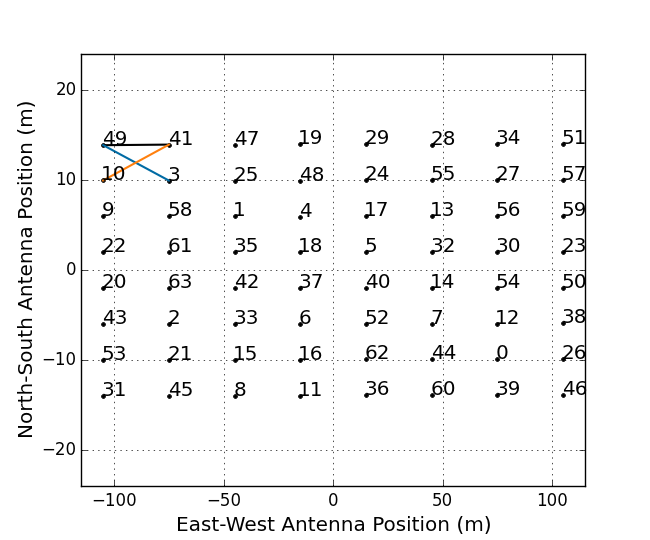
\includegraphics[width=\columnwidth]{plots/antenna_positions.png}
\caption{
Antenna position within the PAPER-64 array.
This analysis only makes use of
east-west baselines between adjacent columns that have row
separations of zero (black; e.g. 49-41, 41-47, 10-3, \dots)
one in the northward direction (orange; e.g. 10-41, 3-47, 9-3, \dots) or
one in the southward direction (blue; e.g. 49-3, 41-25, 10-58, \dots).
Because of their high levels of redundancy, 
these baselines constitute the bulk of the array's sensitivity for power
spectrum analysis.}
\label{fig:antenna_positions}
\end{figure}

\begin{figure*}
%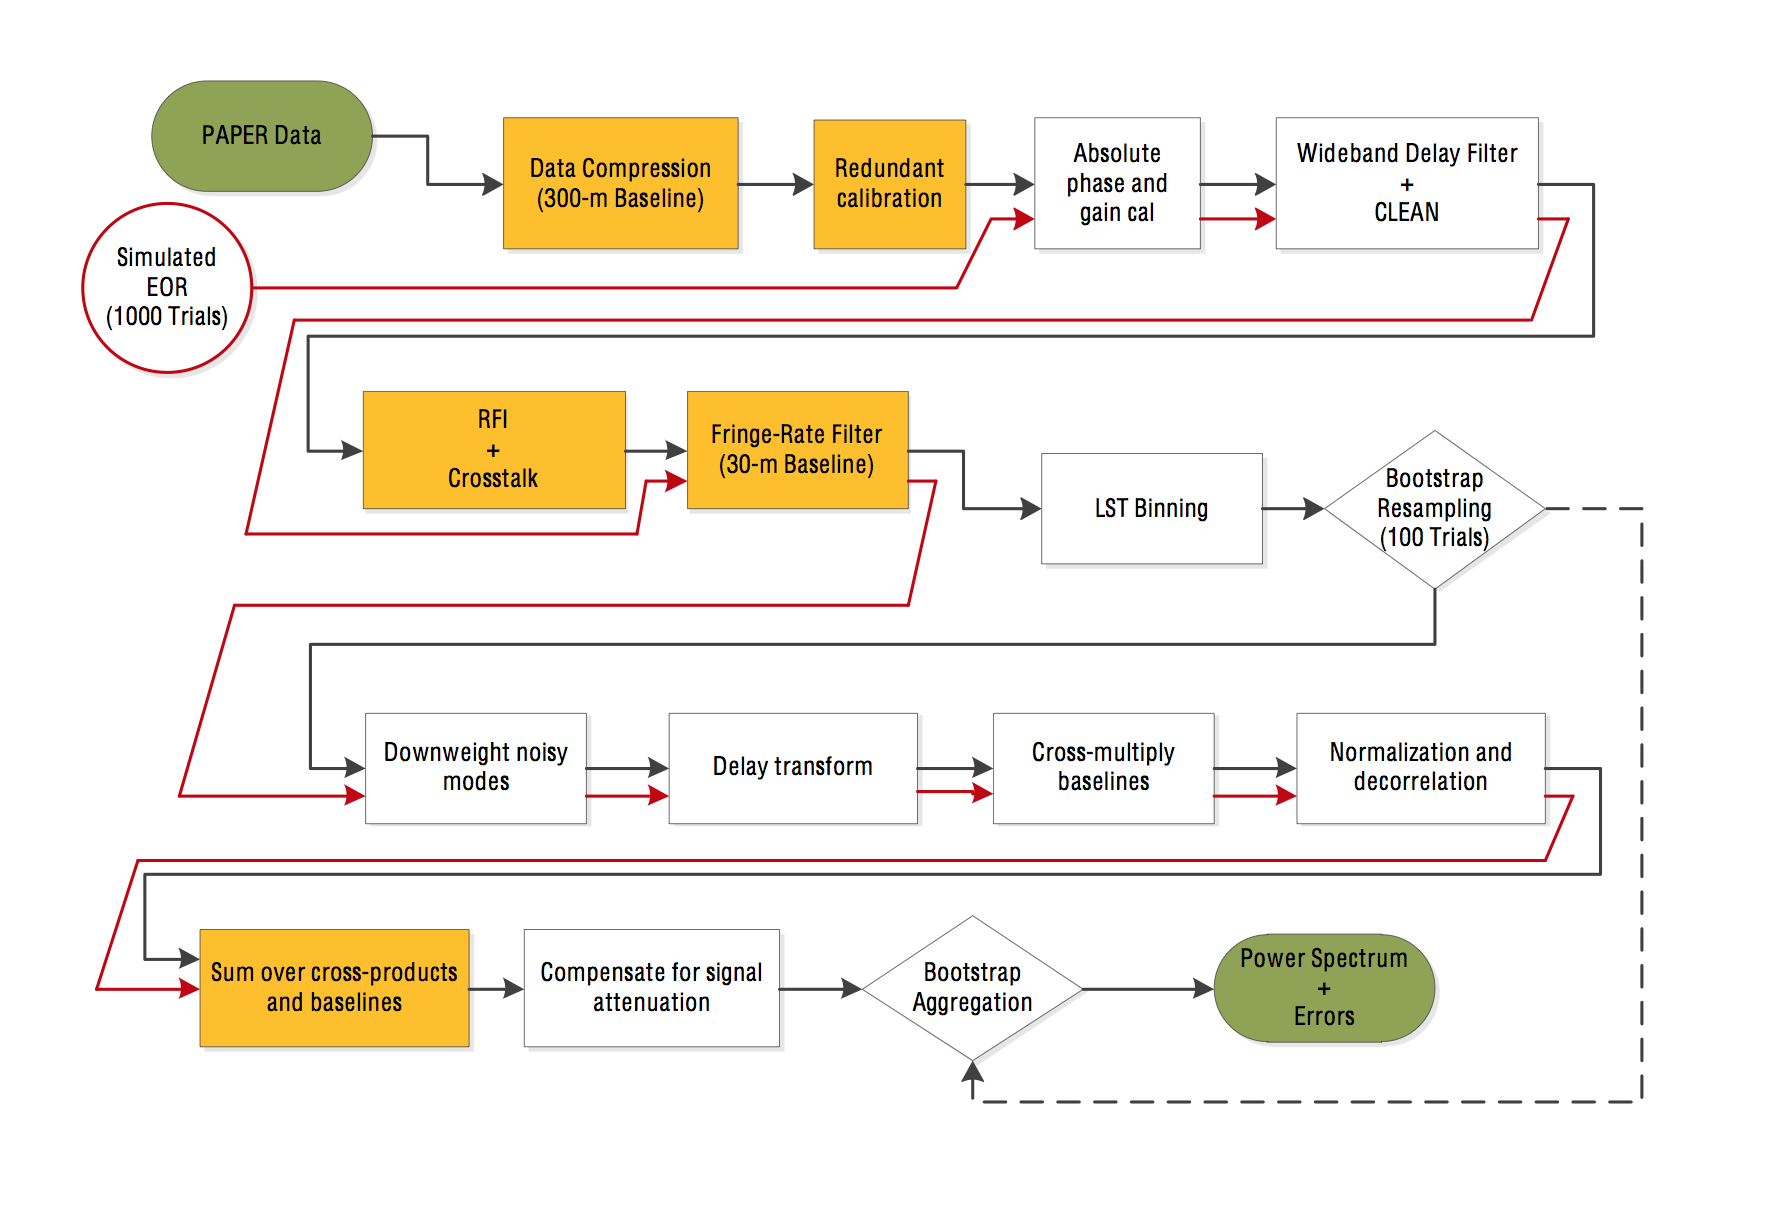
\includegraphics[width=2\columnwidth]{plots/data_flow_chart.png}
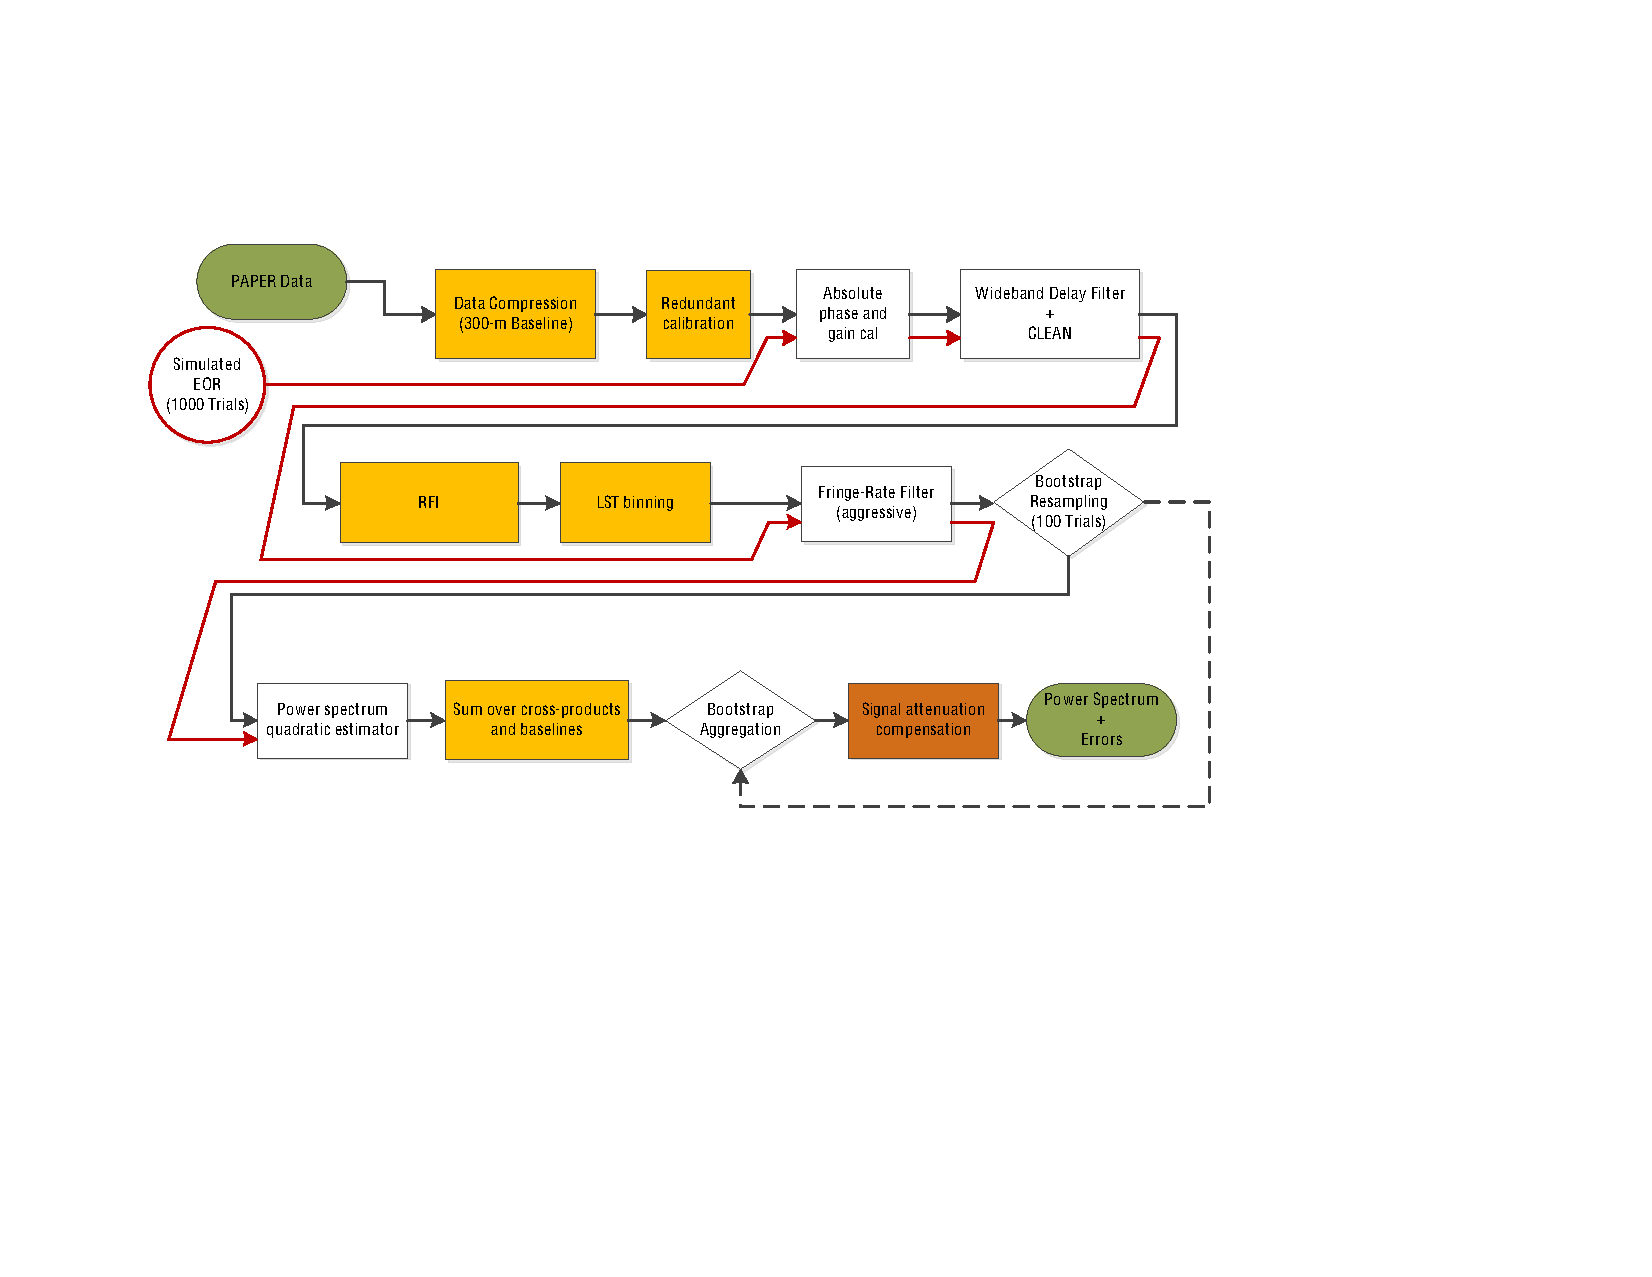
\includegraphics[width=2\columnwidth,trim=0cm 7cm 5cm 2cm,clip]{plots/data_flow_chart.pdf}
\caption
{
The stages of power-spectrum analysis. Black lines indicate data flow; red lines indicate
Monte Carlo simulations used to 
measure signal loss. Yellow boxes indicate stages that by construction have negligible signal loss.
Signal loss in other stages is tabluted in Table \ref{tbl:sigloss}.
}
\label{fig:flowchart}
\end{figure*}

We base our analysis on drift-scan observations 
with 64 dual-polarization PAPER antennas (hereafter, ``PAPER-64") deployed 
at the Square Kilometre Array South Africa
(SKA-SA) reserve in the Karoo desert in South Africa
(30:43:17.5$^\circ$ S, 21:25:41.8$^\circ$ E).
Each PAPER element features a crossed-dipole design measuring two
linear (X,Y) polarizations.
The design of the PAPER element, 
which features spectrally and spatially smooth responses 
down to the horizon with a full-width half-maximum of $60^{\circ}$, is summarized in \citet{parsons_et_al2010}
and \citet{pober_et_al2012}.  
For this analysis, we use only the XX and YY polarization cross-products.

As shown in Figure \ref{fig:antenna_positions}, PAPER-64 employs
a highly redundant antenna layout where multiple baselines measure
the same Fourier mode on the sky (P12a; P14).
We rely on all 2016 baselines for calibration,
but only use a subset of the baselines for the power spectrum
analysis. This subset consists of three types of baselines: the 30-m
strictly east-west baselines between adjacent columns (e.g. 41-47, black 
in Figure \ref{fig:antenna_positions}; hereafter referred to 
as {\it fiducial baselines}), 30-m east-west baselines
whose eastern element is staggered one row up (e.g. 10-41, orange in Figure \ref{fig:antenna_positions}), and
those whose eastern element is one row down (e.g. 10-58, orange in Figure \ref{fig:antenna_positions}) 
\textbf{These baseline groups consist of 56, 49, and 49 baselines, respectively}.
We define a redundant group of
baselines as being the set of baselines that have the same grid spacing;
baselines in each
of the three redundant groups described above are instantaneously redundant and
therefore measure the same Fourier modes on the sky. Thus, within a redundant group,
measurements from baselines may be 
coherently added to build power-spectrum sensitivity as $N$ rather than
$\sqrt{N}$, where $N$ is the number of baselines added.  

PAPER-64 conducted nighttime observations over a 135 day period 
from 2012 November 8 (JD 2456240) to 2013 March 23 (JD 2456375). 
Since solar time drifts with respect to local sidereal time (LST), this observing campaign
yielded more samples of certain LSTs (and hence, sky positions) than others. 
For the power spectrum analysis, we use observations between 0:00 and 8:30 hours
LST.  This range corresponds to
a ``cold patch" of sky away from the galactic center where galactic synchrotron power is minimal,
but also accounts for the weighting of coverage in LST.
Figure \ref{fig:coverage} shows our observing field with the contours labeling
the beam weighted observing time relative to the peak, directly over head the
array.

The PAPER-64 correlator processes a 100--200 MHz bandwidth, first
channelizing the band into 1024 channels of width 97.6 kHz, and then
cross multiplying every antenna and polarization with one another for a total of
8256 cross products, including auto correlations.  Following the architecture 
in \citet{parsons_et_al2008}, this
correlator is based on CASPER\footnote{\url{http://casper.berkeley.edu}} open-source
hardware and signal processing libraries \citep{parsons_et_al2006}.  
Sixteen ROACH boards each hosting eight 8-bit analog-to-digital
converters digitize and channelize antenna inputs. New to this correlator relative to previous PAPER correlators \citep{parsons_et_al2010},
the cross multiplication engine is implemented on eight servers each receiving
channelized data over two 10-Gb Ethernet links.  Each server hosts
two NVIDIA GeForce 580 GPUs running the open-source cross-correlation code developed
by \citet{clark_et_al2013}.
Visibilities are integrated for 10.7 s on the GPUs before
being written to disk.  All polarization cross-products are saved, although the
work presented here only made use of the XX and YY polarization products.

\begin{figure*}\centering
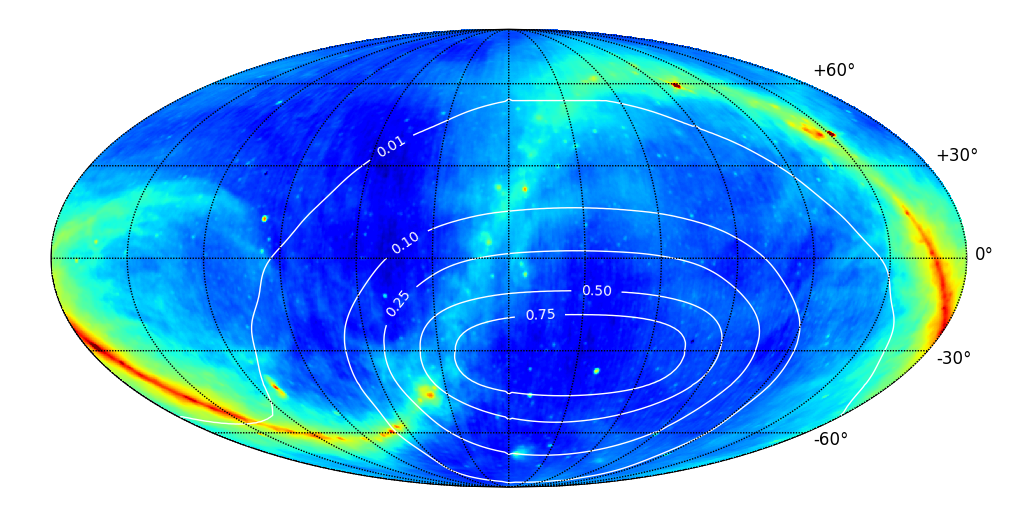
\includegraphics[width=2\columnwidth]{plots/coverage.png}
\caption{The Global Sky Model \citep{deoliveira2008}, illustrating foregrounds to the 21cm
cosmological signal, with 
contours indicating beam-weighted observing time (relative to peak) for the PAPER observations
described in Section \ref{sec:observations}.  The map is centered at 6:00 hours in right ascension.
}\label{fig:coverage}
\end{figure*}


%%%%%%%%%%%%%%%%%%%%%%%%%%%%%%%%%%%%%%%%%%%%%%%%%%%%%%%%%%%%%%%%%%%%%%%%%%%%%%%%
\section{Calibration}\label{sec:calib}

Foreground contamination and signal sensitivity represent the two major concerns for 21~cm
experiments targeting power spectrum measurements. Sources of foregrounds include
galactic synchrotron radiation, supernova remnants, and extragalactic radio sources.
In the low-frequency radio band (50--200 MHz) where 21~cm reionization
experiments operate, emission from these foregrounds is brighter than the
predicted reionization signal by several orders of magnitude
\citep{santos_et_al2005,ali_et_al2008,deoliveira2008,jelic_et_al2008,bernardi_et_al2009,bernardi_et_al2010,ghosh_et_al2011}.
However, the brightest foregrounds are spectrally smooth, and this provides an
important hook for their isolation and removal
\citep{liu_et_al2009,petrovic_oh2011,liu_tegmark2012}.  Unfortunately,
interferometers, which are inherently chromatic
instruments, interact with spectrally smooth foregrounds to produce unsmooth features that
imitate line-of-sight Fourier modes over cosmological volumes (P12b; \citealt{bowman_et_al2009,morales_et_al2006a}).
One approach to solving this problem involves an ambitious calibration and modeling approach to spatially localize and
remove foreground contaminants 
\citep{bowman_et_al2008,liu_et_al2008,harker_et_al2009,sullivan_et_al2012,chapman_et_al2013}.
Perhaps the most impressive example of this approach is being undertaken by LOFAR, where dynamic ranges of 4.7 
orders of magnitude have
been achieved in synthesis images \citep{yatawatta_et_al2013}, although it is expected that additional
suppression of smooth-spectrum foreground emission will be necessary \citep{chapman_et_al2013}.

The analysis for this paper employs a contrasting
approach based on the fact that the chromaticity of an interferometer
is fundamentally related to the length of an interferometric baseline.  This relationship, known
colloquially as ``the wedge", was 
derived analytically (P12b; \citealt{vedantham_et_al2012,nithya_et_al2013,liu_et_al2014a,liu_et_al2014b}), and has been confirmed in 
simulations \citep{datta_et_al2010,hazelton_et_al2013} and observationally
\citep{pober_et_al2013,dillon_et_al2013b}.  As described in P12b, the wedge is the result of the delay
between when a wavefront originating from foreground emission
arrives at the two antennas in a baseline.  The fact that this delay is bounded by the light-crossing
time between two antennas (which we call the ``horizon limit'' since such a wavefront would have to 
originate from the horizon) places a fundamental bound on the chromaticity of
an interferometric baseline.  So far, PAPER has had the most success in exploiting this bound
(P14; \citealt{jacobs_et_al2014}). 
%although it is in the process of being applied to MWA observations \citep{nitya}.  
In this analysis, we continue to use the properties of the 
wedge in order to isolate and remove smooth
spectrum foregrounds.

As illustrated in Figure \ref{fig:flowchart},
our analysis pipeline begins by running a compression
algorithm to reduce the volume of our raw data by a factor of 70.
As described in Appendix A of P14, this is achieved by first performing statistical flagging to remove
radio frequency interference (RFI) at the 6$\sigma$ level, applying low-pass delay and fringe-rate filters that limit signal variation
to delay scales of $|\tau|\la1 \mu$s and fringe-rate scales of $f\la23$ mHz, and then 
decimating to critical Nyquist sampling rates of 493 kHz along the frequency axis
and 42.9 s along the time axis.  We remind the reader that while information is lost in this compression,
these sampling scales preserve emission between
$-0.5\le k_\parallel\le 0.5\hMpci$ that rotates with the sky, making this an essentially lossless compression 
for measurements of the 21 cm reionization signal in these ranges.

After compression, we calibrate in two stages, as described in more detail below.  
The first stage (Section \ref{sec:relcal}) uses instantaneous redundancy to solve for the majority of the 
per-antenna internal degrees of freedom in the array.  In the second stage (Section \ref{sec:abscal}), standard self-calibration is used 
to solve for a smaller number of
absolute phase and gain parameters that cannot be solved by redundancy alone. 
After suppressing foregrounds with a
wide-band delay filter (Section \ref{sec:wbd_filtering}) and additional RFI flagging and crosstalk removal, 
we average the data in LST (Section \ref{sec:lstbin}) and apply a
fringe-rate filter (Section \ref{sec:frf}) to combine time-domain data. 
Finally, we use an
optimal quadratic estimator (Section \ref{sec:oqe}) to make our estimate of the 21 cm power spectrum.

\subsection{Relative Calibration}\label{sec:relcal}
%    -Principles of redundant calibration. Fact that there is no signal loss in
%       this kind of measurement.
%       --PAPER has a redundant configuration. Therefore the number of baselines
%         is larger than the number of unique baselines in the array. There are
%         multiple baselines that measure the same sky.
%       --Introduce uniqe baseline. We define a unique baseline to be the set of
%         redundant baselines of a unique orientation.
%       --All baselines of a unique baseline measure the same sky and
%         therefore, differences between them are what need to be calibrated
%         out. These are the gain variations imparted on the incoming signal by
%         the antenna.
%       --There is no signal loss in this method. Sky signal is the same for
%         each of the redundant baselines is the same and hence any algorithm that
%         preserves common mode signal (which is what redcal does) is necessarily
%         lossless. This is an important point!  
%       --In addtion, because gains are normalized to have a unity magnitude the
%         input arn output flux scale are the same. (This is an omnical thing)
%         
%    -What can we solve for and what can't we solve for. We can solve for the
%     relative complex gains between antennas, but not the absolute gain and phase.
%       --Because redundant calibration does not fold in any outside
%         information about the sky that we are observing, it inherently is a
%         relative calibration scheme that solves for the relative gains and
%         phases of antennas within the array. 
%       --Therefore, we cannot solve for the absolute phase and gain of the
%         array. There is not enough information.
%       --Absoulte phase and gain calibration are addressed in later sections.
%

Redundant calibration has gained attention recently as a particularly powerful
way to solve for internal degrees of freedom in radio interferometric measurements without simultaneously
having to solve for the distribution of sky brightness 
(\citealt{wieringa1992,liu_et_al2010,noorishad_et_al2012,marthi_chengalur2014,zheng_et_al2014}; P14).
The grid-based configuration of PAPER antennas allows a large number of antenna
calibration parameters to be solved for on the basis of redundancy (P14; P12a; 
\citealt{zheng_et_al2014}).  Multiple baselines of the same length and
orientation measure the same sky signal. Differences between redundant
baselines result from differences in the signal chain, including amplitude and
phase effects attributable to antennas, cables, and receivers.  Redundant
calibration only constrains the relative complex gains between antennas and is
independent of the sky. Since redundant calibration preserves signals common to
all redundant baselines, this type of calibration does not result in signal loss.

%    -Summary of the procedure of redundant calibration. This should be mixed in
%     with the equations from Zheng et. al.
%       --Two flavors of redundant calibration : logcal and lincal. Cite
%         liu,zheng.
%       --logcal takes log of equation 3 in zheng et. al., and thus becomes a
%         linear system. Can then solve for the log of the antenna gains, as
%         well as the true visibility of the sky as measured from a unique
%         baseline. 
%       --lincal is the linearization via taylor expansion of the same equation
%         3. This provides us with a better solution. The reason for doing
%         lincal is that logcal is a biased estimator. 
%       --Because there are more baselines than the number of unique baselines, 
%         we have an overdetermined system of equations and therefore can
%         uniquely solve for all of the gains and "true" visibilities.

In practice, redundant calibration often takes on two flavors: log calibration (LOGCAL) and
linear calibration (LINCAL) \citep{liu_et_al2010,zheng_et_al2014}. LOGCAL uses 
logarithms applied to visibilities, 
\begin{equation}
    v_{ij} = g_{i}^{\ast}g_{j}y_{i-j} + n_{ij}^{res},
\end{equation}
where $g$ denotes the complex gain of antennas indexed by $i$ and $j$, and $y$
represents the ``true" visibility measured by the baseline, to give
a linearized system of equations
\begin{equation}\label{eqn:logcal}
    \log{v_{ij}} = \log{g_{i}^{*}} + \log{g_{j}} + \log{y_{i-j}},
\end{equation}
In solving for per-antenna gain parameters with
a number of measurements that scales quadratically with antenna number, redundancy gives 
an over-constrained
system of equations that can be solved
using traditional linear algebra techniques.
While LOGCAL is useful for arriving at a coarse solution from initial estimates that are far
from the true value, LOGCAL has the shortcoming of being a biased by the asymmetric behavior
of additive noise in the logarithm \citep{liu_et_al2010}.

LINCAL, on the other hand, uses a Taylor expansion of the visibility around initial
estimates of the gains and visibilities, 
\begin{equation}\label{eqn:lincal}
v_{ij} = g_{i}^{0*}g_{j}^{0}y_{i-j}^{0} + g_{i}^{1*}g_{j}^{0}y_{i-j}^{0} +
         g_{i}^{0*}g_{j}^{1}y_{i-j}^{0}+g_{i}^{0*}g_{j}^{0}y_{i-j}^{1},
\end{equation}
where $0$ denotes initial estimates and $1$ represents the perturbation to the
original estimate and is the solutions we fit for.  Using initial estimates
taken from LOGCAL, LINCAL constructs an unbiased estimator.

%    -How was this calibration applied to the data. 
%       --Using omnical package. Give credit jeff and url to omnical. Cite
%         paper.
%       --Implements both logcal and lincal. Discuss the speed ups. 
%       --gains were applied to the uv datasets and written out in the same
%         format. However, Omnical is quite general and solutions can be written
%         out in text files and adapted to other file formats.
%    
%    -Removing additive offset and what is the time cadence of all of this.
%       
%    -Diagnostic figures : Chi-squared, complex plane, stability vs. time and
%                          frequency.

Redundant calibration was performed using 
OMNICAL\footnote{https://github.com/jeffzhen/omnical} --- an open-source
redundant calibration package that is relatively instrument agnostic
\citep{zheng_et_al2014}. This package implements both LOGCAL
and LINCAL, solving for a complex gain solution per antenna, frequency, and
integration. The solutions are then applied to visibilities and the results are
shown in Figure \ref{fig:omniview}.

\begin{figure*}
\centering
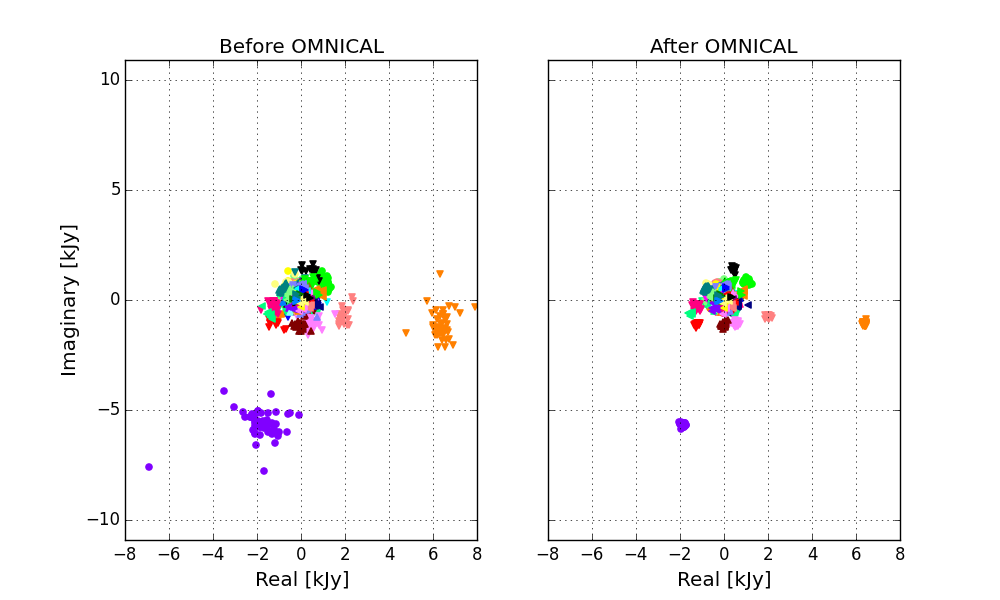
\includegraphics[width=1.5\columnwidth]{plots/omniview_64.png}
\caption{
%ARP: overriding this change. making this point is not worth the loss of clarity
PAPER visibilities plotted in the complex plane before (left) and
after (right) the 
application of the improved redundancy-based calibration with OMNICAL
\citep{zheng_et_al2014}.  All baselines in the array measured at 159 MHz for a
single time integration are plotted.  Instantaneously redundant baselines are
assigned the same symbol/color.  The tighter clustering of redundant
measurements with OMNICAL indicates improved calibration.
} 
\label{fig:omniview}
\end{figure*}

\begin{figure}
\centering
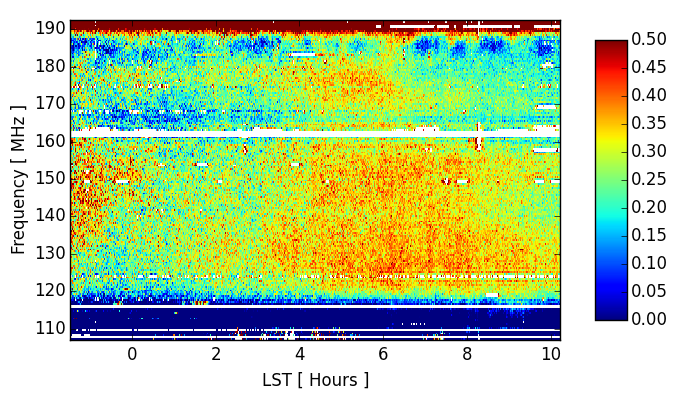
\includegraphics[width=\columnwidth]{plots/chi2.png}
\caption{
Log of $\chi^{2}$ per degree of freedom of all baseline residuals after the application of OMNICAL.
The plot comprises a observations over one day, with a frequency resolution of
493 kHz and a time resolution of 42.9 s.
} \label{fig:chi2}
\end{figure}

In addition to solving for gain solutions, OMNICAL also characterizes the
quality of the calibration parameters by calculating the $\chi^{2}$ for every
integration. As defined in \citet{zheng_et_al2014}, 
\begin{equation}\label{eqn:chi2}
    \chi^{2} = \sum_{ij}\frac{|v_{ij} - y_{i-j}g^{\ast}_{i}g_{j}|^{2}}{\sigma^{2}_{ij}},
\end{equation}
where $\sigma^{2}$ is the noise in the visibilities. The $\chi^{2}$
measures sum of the deviation of measured visibilities to that of the best fit model
derived from the LINCAL relative to a noise model, and gives us a tool to use in order to check the
quality of our data. The number of degrees of freedom (DoF), as defined in \citealt{zheng_et_al2014}, is given by 
\begin{align}
    \text{DoF} &= N_{\text{measurements}} - N_{\text{parameters}} \\\notag
               &= 2N_{\text{baselines}} - 2(N_{\text{antennas}} + N_{\text{unique baselines}}),
\end{align} 
and is effectively the number of visibilities for which
$\chi^{2}$ is calculated. If the data are noise-dominated, 
$\chi^{2}/\text{DoF}$ is drawn from a $\chi^{2}$ distribution with $\mu=1$ and
$\sigma^{2} = 2/\text{DoF}$. The calculated $\chi^{2}/\text{DoF}$ for every
frequency and integration of a fiducial day of observation in this season and
for the fiducial power spectrum baselines is shown in Figure \ref{fig:chi2},
demonstrating the stability of the PAPER instrument.


We measure a mean $\chi^{2}/\text{DoF}$ of 1.9.  This
indicates that the redundant calibration solutions, while a substantial improvement
over the previous PAPER-32 calibration (P14), do not quite result in residuals that are thermal noise dominated.
Possible sources of this excess include instrumental crosstalk and poorly performing signal chains.
While the latter will be down-weighted by the inverse of the estimated signal covariance described
in Section \ref{sec:oqe}, crosstalk is a defect in the data that must be addressed.
% ARP: removing this discussion because this was not used on the data, so irrelevant
%Large values of the $\chi^{2}$ can correspond to various systematics in the
%data. One systematic is radio frequency interference (RFI) that are
%sporadically triggered in both time and frequency due to terrestrial sources.
%In this regime, redundant baselines would agree on RFI spikes in frequency and
%time and therefore the residuals from the redundancy would be low. However,
%noise models usually only contain the noise within the system and true sky. In
%this case, the noise would underestimate the noise in the measurement and cause
%a large $\chi^{2}$. In this way, the $\chi^{2}$ can be used as a metric to
%search and flag RFI: if certain integrations and frequencies have a large
%$\chi^{2}$ for some percentage of redundant baselines, then we could with high
%confidence flag out those data points. The data set presented in this paper did
%not use this method for flagging.
%redundant baselines are not redundant with one another, owing to some
%systematic such as cross talk, or two, a strong signal such as radio frequency
%interference (RFI), in which case the noise is underestimated, even though all
%baselines may agree in the RFI, producing a large $\chi^{2}$. Figure
%\ref{fig:chi2} shows the logarithm of $\chi^{2}$ for all frequencies for and an entire
%night of observation. The noise model used was the variance of the visibilities for
%a given frequency and LST bin. As discussed, the $\chi^{2}$ can be a metric used
%for RFI flagging and removal because when RFI dominates, at a given frequency or
%time, the $\chi^{2}$ would be large. Therefore, if some percentage of redundant
%baselines agree on the large $\chi^{2}$, then we can flag them out of our data
%on that basis. This data set did not use the $\chi^{2}$ as a metric but
%preliminary studies have shown it's efficacy on PAPER-128 observations.
Crosstalk caused by the cross-coupling of signals between antennas
reveals itself as a static complex bias to a
visibility that varies on timescales much longer than typical fringe rates.
This effect 
skews the distribution of the $\chi^2$ of the residuals away from 1.
To minimize crosstalk, we first use OMNICAL to solve for antenna-dependent gains,
and then average the residual deviations from redundancy
over 10-minute windows before subtracting
the average from the original visibilities. This
crosstalk removal preserves signals common to redundant baseline groups (such as the 21 cm signal).
Unfortunately, it also preserves a term that is the average of the crosstalk of all baselines
in the redundant group.  This residual crosstalk is removed by a fringe-rate filter later
in the analysis.

\subsection{Absolute Calibration}\label{sec:abscal}
%    -Selfcal to pictor, fornax, and crab (to get the north-south components).
%       --Reiterate that redundant cal does not solve for the overall flux and
%         phase parameters. 
%       --There are two final phase parameters we must solve
%         for in order to correctly phase to a source on the sky. Redundancy
%         only gets you so far, but still need to be able to unambiguously phase
%         to sources.
%       --We use self calibration to solve for the global phase parameters using
%         Pictor A, Fornax A, and Crab Nebula. 
%       --
%
%    -Diagnostic Plots: Show Field image from Bernardi. This will give
%     confidence in a good absolute phase calibration.

After solving for the relative complex gains of the antennas using redundant
calibration, an overall phase and gain calibration remains unknown. We use the
standard self calibration method for radio interferometers to solve for the
absolute phase calibration. We used Pictor A, Fornax A, and the Crab Nebula to
fit for the overall phase solutions. Figure \ref{fig:field_image} shows an image
of the field with Pictor A (5:19:49.70, -45:46:45.0)  and Fornax A
(3:22:41.70,-37:12:30.0).
%The measured source positions are the same as the catalogue positions for these sources.

%    -Calibrated to Pictor A. 
%       --As before, redundant calibration cannot set a global flux scale. For
%       our measurements to be correct, we need to set a fluxscale. We use
%       Pictor A to set our fluxscale. Cite Dannys pictor paper.
%      
%    -Our bandpass model is a 9th degree polynomial. 
%       --In order to set our fluxscale, we beamform our data upto pictor A,
%         summing baselines, and then then fit a 9th degree polynomial to the
%         bandpass. This is our measure of the spectrum of Pictor A. 
%       --Because we are beamforming to pictor and fitting a polynomial to the
%         bandpass, there is signal loss. This signal loss is of the 
%    -Tabulate signal loss due to this model. Averaging over Nbls, times gives us
%     an average over independent uv modes.
%       --Working on this... a few questions about it.
%
%    -The actual signal loss on a given mode is L/N where L is the loss for a
%     single instance of the beamform (one time, one baseline) and N is the
%     number of baseline and times that were summed.
%
%    -PLOTS: 
%        --A plot that is the phased to pictor beamform gain 
%          (or maybe just a single channel for all days.
%        --The measured and theoretical pictor spectrum 
%        --A comparison to the PSA32 Flux CAL.

We then set our over all flux scale by using Pictor A as our calibrator source
with source spectra derived in \citet{jacobs_et_al2013}, 
\begin{equation}
    S_{\nu} = S_{150}\times\left(\frac{\nu}{150MHz}\right)^{\alpha},
\end{equation}
where $S_{150} = 381.88~\text{Jy} \pm 5.36$ and $\alpha = -0.76 \pm 0.01$, with
1$\sigma$ error bars.


%To derive the source spectrum from our measurements, we use lst averaged data (see
%section \ref{sec:lstbin}) containing foregrounds for the hour before and after from
%where Pictor A transits. We image, in 15 minute snapshots for this data set,
%every frequency channel. The source spectra is derived per snapshot and we average
%these together, weighting by the primary beam in the direction of Pic A to get
%the measured spectrum of Pictor A. To fit our bandpass, we divide the model
%spectrum with ourAmeasured spectrum and fit a ninth-order polynomial over a
%frequency range from 120-170MHz. Figure \ref{fig:pic_spec} shows the derived
%Pictor A spectrum and the model spectrum derived from \cite{jacobs_et_al2013}.

To derive the source spectrum from our measurements, we use data that have been
LST-averaged prior to the wide-band delay filter described in Section
\ref{sec:wbd_filtering}, for the hour before and after the transit of Pictor A.
We image a $30^\circ \times 30^\circ$ field of view for every frequency channel
for each 10 minute snapshot and apply uniform weights to the gridded
visibilities. We account for the required three dimensional Fourier transform in
wide field imaging by using the w-stacking algorithm implemented in WSclean
\citep{offringa_et_al2014} – although we note that the standard w-projection
algorithm implemented in CASA\footnote{http://casa.nrao.edu} gives similar
performances as the PAPER array is essentially instantaneously coplanar.  A
source spectrum is derived for each snapshot by fitting a two dimensional
Gaussian to Pictor A by using the
PyBDSM\footnote{http://www.lofar.org/wiki/doku.php?id=public:user\_software:pybdsm}
source extractor. Spectra are optimally averaged together by weighting them with
the primary beam model evaluated in the direction of Pictor A. To fit our
bandpass, we divide the model spectrum by the measured one and fit a 9th order
polynomial over the 120-170 MHz frequency range. Figure \ref{fig:pic_spec} shows
the calibrated Pictor A spectrum and the model spectrum from
\citet{jacobs_et_al2013}. Also plotted are the $1\sigma$ error bars derived from the PyBDSM source extractor and averaged over the multiple snapshots used after being weighted by the beam-squared.

\begin{figure}
\centering
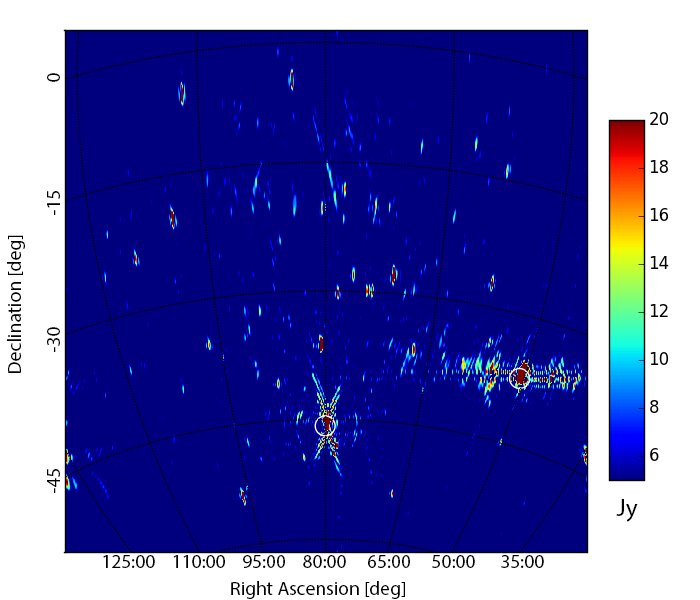
\includegraphics[width=\columnwidth]{plots/picimg_cs.png}
\caption{
PAPER-64 image of a field including Pictor A and Fornax A, with white circles
indicating catalog positions \citep{jacobs_et_al2011}. Image was synthesized with two hours
of visibilities while Pictor A was in transit and 53 MHz of instantaneous
bandwidth from 120 to 173 MHz.  Image quality is limited by the redundant
configuration of the array (e.g. grating lobes as a result of periodic antenna
spacing, elongated lobes arising from poor uv-coverage in the north-south
direction).  Nonetheless, this image demonstrates accurate phase calibration
over a wide field of view.
} \label{fig:field_image}
\end{figure}


\begin{figure}
\centering
%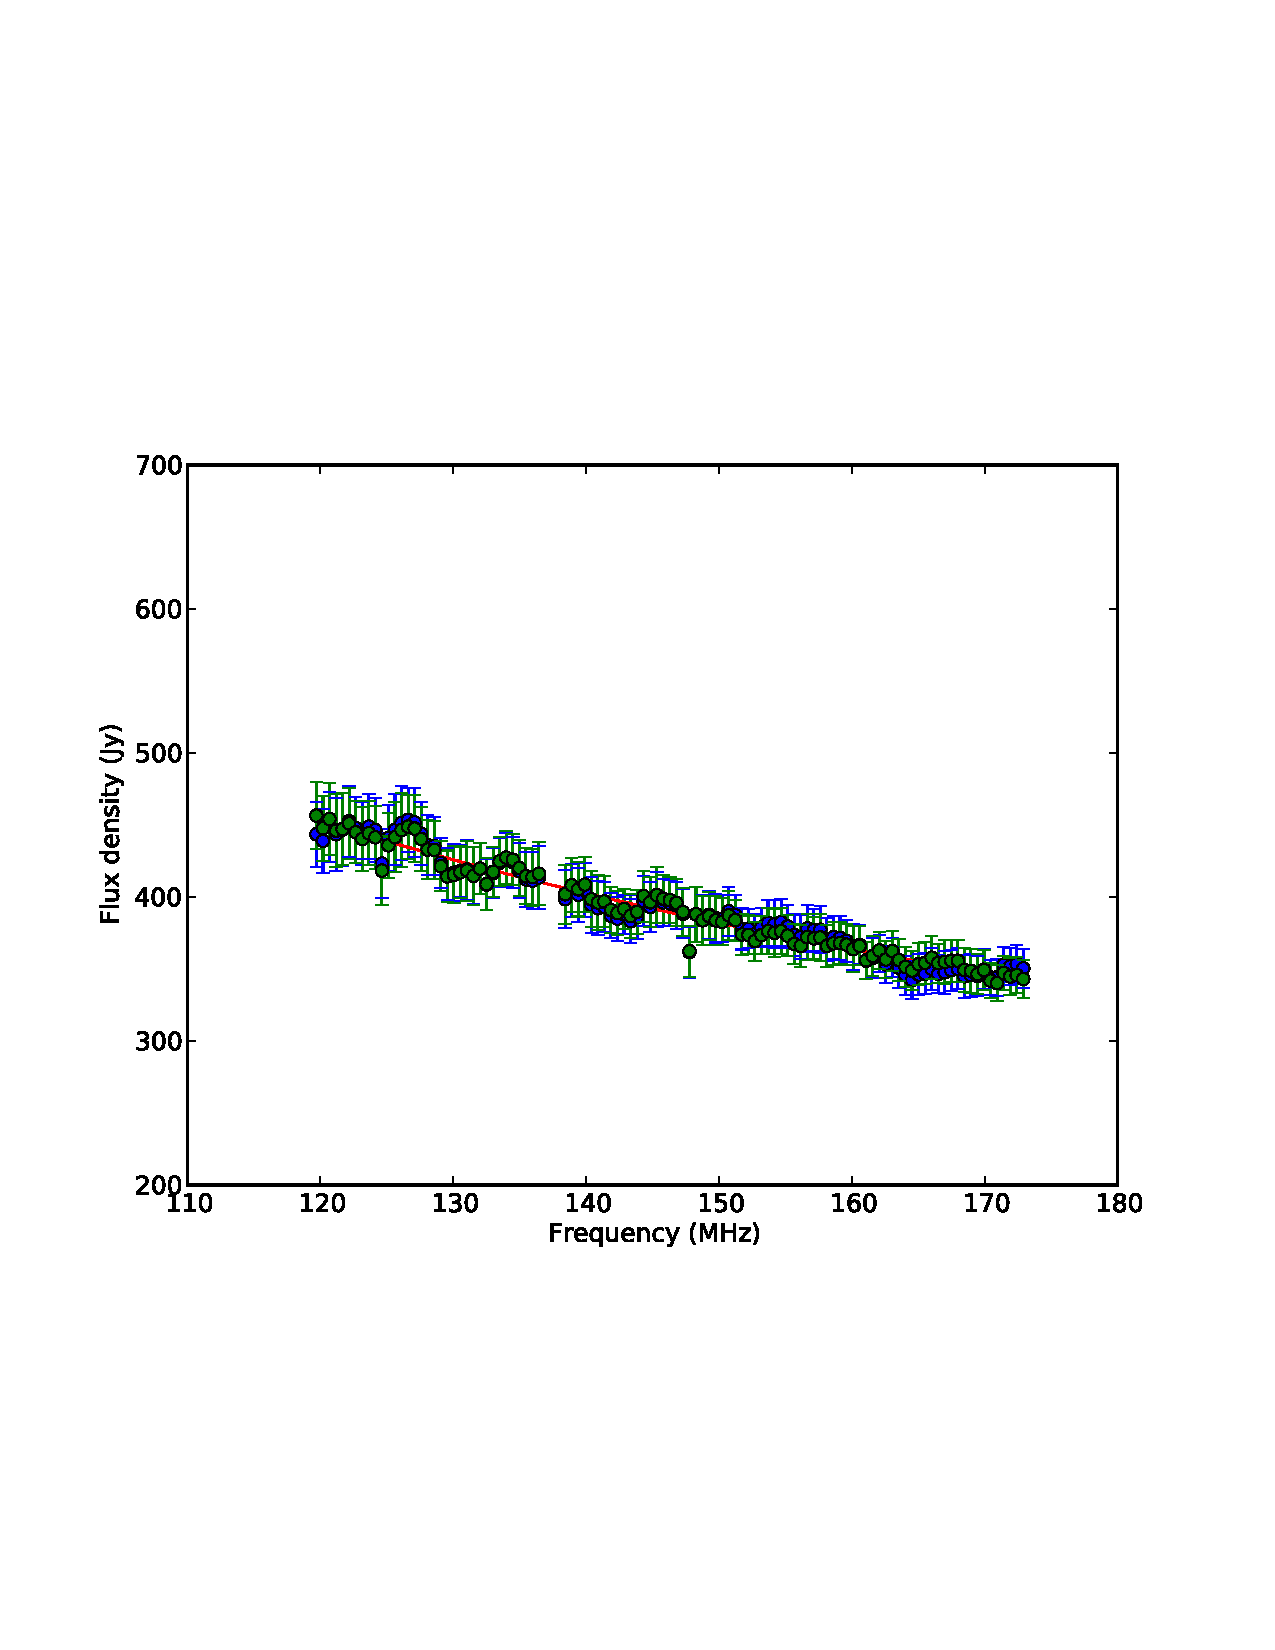
\includegraphics[width=\columnwidth]{plots/PicA_normalized_spectrum.pdf}
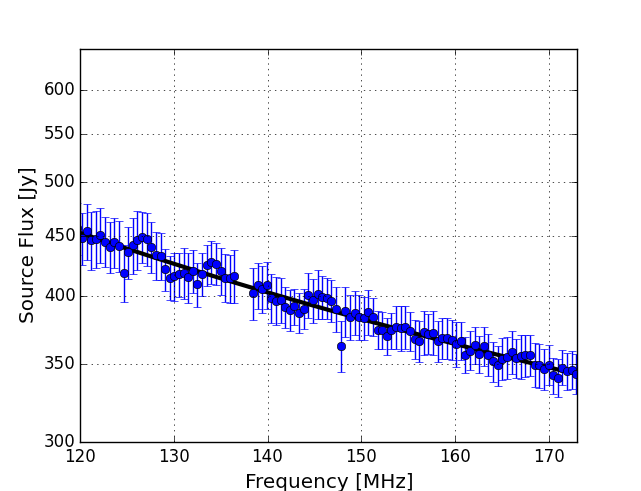
\includegraphics[width=\columnwidth]{plots/picspec.png}
\caption{
Measured spectrum of Pictor A in Stokes I (blue) relative to its catalog
value (black; \citealt{jacobs_et_al2013}).  Flux density measurements are
extracted from images of Pictor A, made independently for each frequency channel in
10 minutes snapshots as Pictor transits between hour angles of -1:49
and 1:10.  Each measurement is then divided by the PAPER beam model and
averaged to obtain the measured spectrum, which serves to characterize the flux
scale of the PAPER-64 observations. Error bars indicate 68\% confidence
intervals, derived from the Gaussian fits in the source extractor used to
measure the flux density in PyBDSM, combined from all snapshots.
}\label{fig:pic_spec}
\end{figure}


Fitting a polynomial to the bandpass has the potential for signal loss which
would include suppressing modes that may contain the cosmological signal. In order to
quantify the signal loss associated with fitting a ninth degree polynomial to
the bandpass, we run a Monte Carlo simulation of the effect the bandpass has on
a model 21-cm reionization signal. We construct a model baseline visibility as a Gaussian
random signal 
multiplied by the derived bandpass for every independent mode measured. We
calculate the total number of independent modes by counting the number of
independent uv-modes sampled for the different baseline types over the two hour
time interval used to measure the bandpass. We average each mode together and
fit a 9th degree polynomial. Using this as our measured bandpass for this
simulated signal, we finally compare the power spectrum from the output of the
simulated signal to the input power spectrum as a function fo $k$-mode.  We
find that between $-0.06 < k < 0.06$, the width of our wideband delay filter
described below, the signal loss is less than $3\%$ and at the mode right
outside the above limit is $2\times{10^{-7}}\%$. We apply the latter correction
factor for all modes outside the width of the delay filter to the final power
spectrum.


%These lists were My bullet points.
%\begin{itemize}
%    \item{Overview of the calibration with emphasis on Omnical.}
%    \item{Rough Calibration : Can cite Parsons 2014 for the details.}
%    \begin{itemize}
%        \item{Discuss the first pass of redundant phase and gain calibration.
%              Absolute phase calibration using pictor, fornax and crab in the
%              fit.}
%        \item{Absolute flux scale using Pictor A. Want to address signal loss.
%             Maybe delay the issue of signal loss to a "Signal Loss" section
%             which takes into account the signal loss in various stages of the 
%             analysis?}
%        \item{Add in details of the loss of eor signal. Do simulations to get
%              numbers. }
%        \item{Plots : Measured pictor spectrum with comparison to the Danny
%              pictor spectrum. Maybe some simulation plots showing the signal
%              loss due to the polynomial fit to pic spec.}
%    \end{itemize}
%    \item{Omnical}
%    \begin{itemize}
%        \item{What is omnical?}
%        \item{Why are we using it? To get a frequency/time dependent
%calibration. Need to address why this is not overfitting. That is why is this
%just not flatting everything out.}
%        \item{Address non-possibility of signal loss.}
%        \item{Refresh formalism (do this here or in the intro of calibration?)}
%        \item{What is it doing? logcal/lincal. Chi-squared and how that
%              determines the goodness of the fits to the model baselines. What
%model are we using? Is it a good model?}
%        \item{Plots: Chi-squared plots. Compex plane plots that show
%              improvements over uncalibrated/rough/omnical calibrated. 
%              Time and frequency stability.}
%    phase to pic gain, pic spec, comparison to psa32.
%    \end{itemize} 
%\end{itemize}

%OLD TEXT START
%\subsubsection{Overview}
%As the name suggests, redundant calibration (\cite{liu_et_al2010},
%\cite{zheng_et_al2014}) uses redundancy within the array to solve for relative
%phases and gains of the antennas. To explain redundant calibration, suppose that
%the baseline between antennas $i,j$ measure a visibility $v_{ij}$, then we have 
%
%\begin{equation}\label{eqn:redcal}
%    v_{ij} = g_{i}g_{j}^{*}y_{i-j} + n_{ij},   
%\end{equation}
%where $g_{i}$,$g_{j}$ are the complex gains due to antenna $i$ and antenna $j$,
%respectively, $y_{i-j}$ is the true visibility measured by perfect antennas
%$i$,$j$ for the given baseline type, and $n_{ij}$ is the residual noise from
%the baseline.  If the number of baselines of a given type is much greater than
%the number of baselines types this problem is over constrained and $g_{i}i$,
%$g_{j}$, and $y_{i-j}$ can be solved for. PAPER is in this limit due to the
%maximally redundant configuration as shown in figure \ref{fig:antenna_pos}. 
%
%Redundant calibration comes in two flavors: log calibration and linear
%calibration. Log calibration, or logcal for short, takes the logarithm of
%equation \ref{eqn:redcal} to give a linearized system. Hence, solutions can be
%solved for by using standard linear algebra techniques. However, this method is
%biased. On the other hand linear calibration, or lincal for short, is an
%unbiased method of solving for the complex gain solutions. In this method
%equation \ref{eqn:redcal} is Taylor expanded about an initial guess for the
%$g_{i}$'s and $y_{i-j}$'s to give a linearized equation which can be used to
%solve for the complex gains and sky model. 
%
%In this analysis we used a logcal algorithm based in delay space to get a rough
%calibration of the dataset. This was followed by an absolute calibration to set
%the overall phase and flux scale using a self calibration. We used model phase
%centers of Pictor, Fornax A, and Crab Nebula. The absolute amplitude is set
%by the flux of Pictor A found in \cite{jacobs_et_al2013}, whose spectrum is
%defined by 
%\begin{equation}
%    S_{\nu} = 382(\frac{\nu}{150 MHz})^{-.76} Jy.
%\end{equation}
%
%Finally, we used the Omnical calibration package to do another round of
%redundant calibration to get even more accurate calibration parameters.
%
%\subsection{logcal-for lack of a better title}
%We first perform the same calibration that was
%done in \citep{parsons_et_al2014a}. That is, we use redundancy to do a relative
%phase\footnote{In actuality, we solve for delays to get around phase wrapping
%issues. These delays are applied to visibilities as $e^{2\pi{i}\tau\nu}$}
%calibration between antennas, which removes the electrical delays from cables in
%the signal path. Due to redundancy, we can calibrate out all of the per-antennas
%delays in the signal path relative to two delay parameters which we call
%$\tau_{ns}$ and $\tau_{es}$. These delays are the relative electrical delays
%that correspond to baseline delays in the north-south and east-west component
%for 2 reference baselines (49-10 and 49-41,respectively). These solutions were
%then applied to the data set which was calibrated again with Omnical. 
%
%The application of this calibration to the data set before Omnical was needed
%because in order to calibrate accurately, Omnical needs to have a rough estimate
%for the calibration solutions for every antenna. In \cite{zheng_et_al2014}, a
%model of the sky was used in order get the rough estimate of the solutions.
%Here, we use actual sky data to get the rough calibration. Because the solutions
%are derived from the instrument, we can incorporate into the solutions antenna
%based variations. 
% 
%The antenna based
%delay solutions vary as much as a couple nanoseconds day to day when solutions
%are averaged over hour long timescales withing a day. However, the variations in
%solutions is worse when only averaging over ten minute time scales. Therefore
%need for better calibration is requred.  We use self calibration to derive the
%two unknow parameters, $\tau_{ns}$ and $\tau_{ew}$, by using the Crab Nebula,
%Fornax A, and Pictor A.
%
%Note that there is no possibility of signal loss (see \citep{parsons_et_al2014a}).
%
%\subsection{Gain Calibration}
%Gain calibration was derived on the basis of redundancy and self calibration.
%The phase calibrations described above, simultaneously also calibrated for the
%relative gain variation between antennas. Again we can only calibrate to a fiducial
%antenna (49) whose gain is defined as unity. We then perform a self calibration
%to set the flux scale to Pictor A whose spectrum is derived in
%\citep{jacobs_et_al2013}. We use the same methods describes in \citep{parsons_et_al2014a}.
%
%Figure \ref{fig:bmfom_pic} shows that dataset beamformed to Pictor A, with log
%janskies on the y axis and lst on the xaxis for a frequncy of .1 + (120/203)*.1/203. 
%As can be seen, the day to day variation in the formed beam has a fractional
%spread of about 10$\%$.  This shows the stability of the instrument and the well
%behaved calibration solutions derived above. 
%
%\subsection{Omnical}
%(How did we know that our calibrations were not good enough? Because of the power
%spectrum? PSA32? We did beamform data to pictorA and say that vs LST, the
%beamform matched well day to day with a fractional spread of about 10$\%$) 
%
%The complex gain solutions found in the previous calibration pipeline were
%averaged together in time and one solution per frequency was used for the array.
%This jived with the philosophy that the array was stable in time and frequency.
%However, upon further review of this data set, it seemed more and more likely
%that this was not the case anymore. (Is this even true? What specifically? Think
%Man!) 
%
%Due to clues that showed that our data set had time dependent calibration
%solutions, it was imperative that we do a better job at calibrating our array.
%
%The Omnical redundant calibrator
%package\footnote{https://github.com/jeffzhen/omnical} (omnical) performs
%redundant calibration for every time and frequency in a dataset using both
%logcal and lincal methods as described in \cite{zheng_et_al2014}. It also
%contains methods on the quality of the solutions by providin a chi-square for
%the fits to the data. 
%
%For this dataset, omnical first performed a logcal (again) to attain a solution
%per time and frequency. This solution was passed to lincal which iteratively
%solved for the complex gain solutions. The convergence criteria was when the
%$\chi^{2}$ decreased by less than $.01\%$. The $\chi^{2}$ for the fit used in
%Omnical is given by 
%\begin{equation}
%    \chi^{2} = \sum_{ij}|v_{ij} - y_{i-j}g_{i}^{*}g_{j}|^{2},
%\end{equation}
%
%which differs from normal nomenclature because we are not inverse varaince
%weighting. Note that this $\chi^{2}$ is summing over all baselines and hence 
%giving more weight to higher gains. Note that omnical fits for each of the
%complex gains and the model visibility, $y_{i-j}$,  for a unique baseline.
%Using this information, figure \ref{fig:chi_2} shows that the $\chi^{2}$ is close
%to 1 for all channels and time (for this day of data). need noise model for
%this.
%
%Figure \ref{fig:gain_solutions} shows the gain solutions output by omnical. The
%amplitude of the gains are roughly order unity through out. These are relative
%gains between antennas and hence the over flux scale set to Pictor A is still
%valid. The absolute calibration is still valid. 
%
%Since Omnical outputs a model visibility of what a unique baseline should
%measure, which is derived from the data by removing all of the variation between
%unique types of baselines and averaging, we are able to use these outputs as our
%dataset. Infact, this is what is done. 
%%waterfalls of chi squared and solutions.
%%day to day repeatability.
%%The output of the omnical - 
%%
%OLD TEXT END



\subsection{Wideband Delay Filtering}\label{sec:wbd_filtering}
%   -Can cite Parsons 2014a
%       --We use the same wbd filter as in Parsons 2014a. That is we do a per
%         baseline delay filtering with a buffer of 15 nanoseconds. 
%   -Quantify signal loss. 
%       --I think this is the same as before. Since delay filtering is done on a
%       per baseline basis, the signal loss from the previous paper and this one
%       is the same. We are using the same filter.
%   -PLOTS:
%        --waterfalls of before and after cleaning.
%        --signal loss vs. k_parallel


Before implementing our foreground removal techniques, we combine the two
linear polarizations for an estimate of Stokes I as per \citet{moore_et_al2013}.
Namely, Stokes I can be estimated as 
\begin{equation}\label{eqn:stokesi}
    V_{\rm I} = \frac12(V_{\rm XX}+V_{\rm YY}),
\end{equation}
where $V_{\rm XX}$ and $V_{\rm YY}$ are the visibilities of the two linear
polarizations measured by the interferometer. There are some important caveats
to the estimate of Stokes I provided by Equation \eqref{eqn:stokesi}. One
important caveat is that it neglects the beam asymmetry  between the two linear
polarization states. This mismatch can cause polarization leakage from Stokes
Q into Stokes I, thus contaminating  our measurement of the power spectrum with any polarized emission from the sky.
This effect for PAPER, as shown in \citet{moore_et_al2013}, leaks 4\% of Q in to
I  in amplitude ($2.2\times10^{-3}$ in the respective power spectra).  We take the conservative approach and do not correct for this effect, noting that the leakage of Q in to I will result in positive power, increasing our limits.

Foreground removal techniques discussed in the literature include spectral
polynomial fitting \citep{wang_et_al2006,bowman_et_al2009,liu_et_al2009},
principal component analysis
\citep{paciga_et_al2011,liu_tegmark2011,paciga_et_al2013,masui_et_al2013},
non-parametric subtractions
\citep{harker_et_al2009,chapman_et_al2013}, and inverse
covariance weighting
\citep{liu_tegmark2011,dillon_et_al2013a,dillon_et_al2013b,liu_et_al2014a,liu_et_al2014b}, Fourier-mode filtering \citet{petrovic_oh2011}, and per-baseline delay filtering described in
P12b.  This delay-spectrum filtering technique is
well-suited to the maximum redundancy PAPER configuration which is not
optimized for the other approaches where high fidelity imaging is a
prerequisite.   The delay-spectrum foreground filtering method is described in
detail by P14; its application is unchanged here.  In summary; we Fourier
transform each baseline spectrum into the delay domain  


\begin{align}\label{eqn:delay_transform}
\tilde{V}_\tau &= \int{W_\nu A_\nu I_\nu
                   e^{-2\pi{i}\tau_{g}}\cdot e^{2\pi{i}\tau\nu}d\nu} \\\notag
                %&= \int{W_\nu A_\nu I_\nu
                %   e^{-2\pi{i}\nu(\tau_{g}-\tau)}d\nu} \\\notag
                &= \tilde{W}_\tau \ast \tilde{A}_\tau \ast
                   \tilde{I}_\tau \ast
                   \delta(\tau_{g} - \tau),
\end{align}
where $A_\nu$ is the frequency dependent antenna response, $W_\nu$ is a sampling function
that includes RFI flagging and a
Blackman-Harris tapering function that minimizes delay-domain scattering 
from RFI flagging, and $I_\nu$ is the source
spectrum.  In the delay domain, a point source appears as a $\delta$-function at
delay $\tau_{g}$, convolved by the Fourier transforms of the
source spectrum, the antenna response, and the
sampling function. We note that the antenna response effectively determines a finite bandpass,
which imposes a lower bound 
of $1/B \approx 10\,\textrm{ns}$ on the width of any delay-domain convolving kernel.
As per
\citet{parsons_backer2009} and P14, we deconvolve the kernel
resulting from $W(\tau)$ using an iterative CLEAN-like procedure
\citep{hogbom1974} restricting CLEAN components to fall within the horizon plus
a 15-ns buffer that includes the bulk of the kernels convolving the $\delta$-function
in Equation \eqref{eqn:delay_transform}.
To remove the smooth spectrum
foreground emission we subtract the CLEAN components from the original
visibility.

\begin{figure*}
\centering
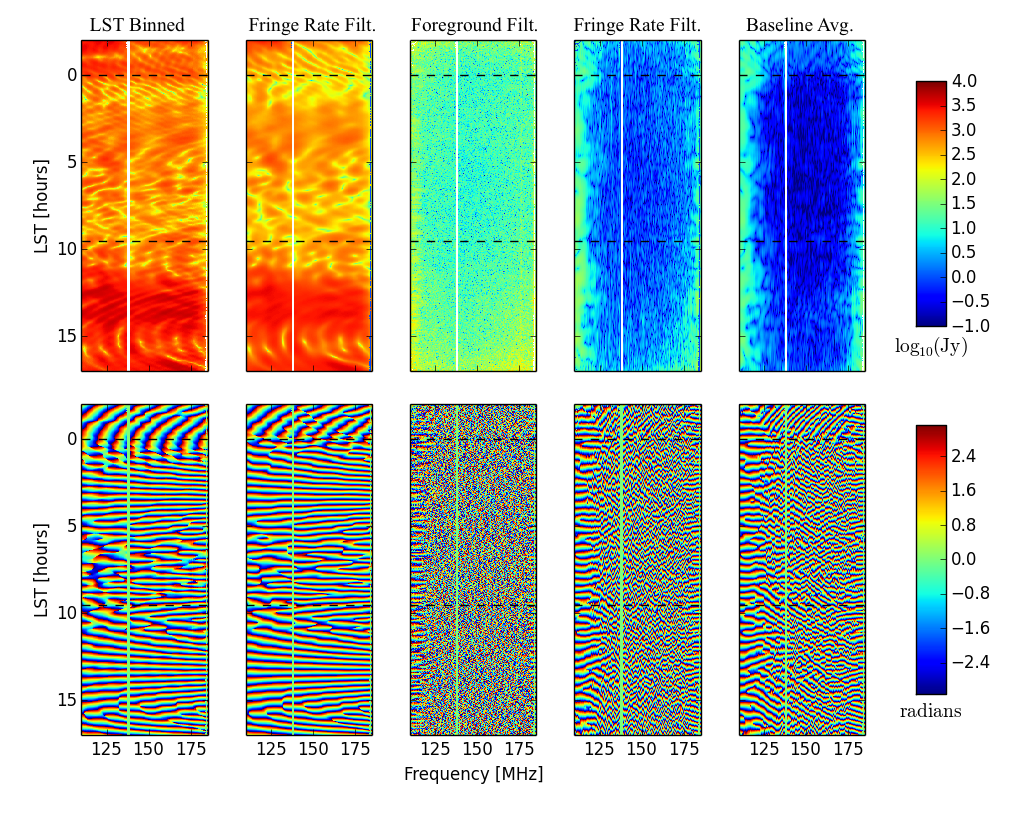
\includegraphics[width=2\columnwidth]{plots/waterfalls_labeled.png}
\caption{
Visibilities measured by a fiducial baseline in the PAPER-64 array, 
averaged over 135 days of observation.  From left to right, columns represent
data that: (1) contain foregrounds prior to the application of a wideband
delay filter or fringe-rate filtering, (2) are fringe-rate filtered but
not delay filtered, (3) are delay filtered at 15 ns beyond the horizon limit but
are not fringe-rate filtered, (4) are both delay and fringe-rate filtered,
and (5) are delay and fringe-rate filtered and have been averaged over all
redundant measurements of this visibility.  The top row shows signal amplitude
on a logarithmic scale; the bottom row illustrates signal phase.
Dashed lines indicate the 0:00--8:30 range in LST used for power spectrum
analysis. The putative crosstalk is evident in the center panel as constant
phase features which do not fringe as the sky.  The two right panels show some
residual signal in the phase structure which is present at low delay. Away from
the edges of the observing band, over four orders of magnitude of foreground
suppression is evident.
} \label{fig:waterfalls}
\end{figure*}

Applying the delay filter to fiducial baselines used in the power spectrum analysis,
foregrounds are suppressed by $\sim$4 orders of magnitude in power, or
 $-40$ dB of foreground suppression, as seen in Figure
\ref{fig:waterfalls}. As discussed in P14, there is a small amount of signal loss
associated with this filter. For the baselines and filter parameters used, the loss was found to be 4.8\% for the
first mode outside of the horizon, 1.3\% for the next mode out, and less than
0.0015\% for the higher modes.  

\subsection{Binning in LST}\label{sec:lstbin}

After the wideband delay filter, we remove a second layer of RFI 
 which was overshadowed by the foreground signal. RFI are excised with a filter
which flags values $3\sigma$ above the median using a variance calculated in a
localized time and frequency window.  

We then average the entire season in LST with 43-s bin widths, matching the
cadence of the compressed data. The full season was 135 days long; of these,
124 days were included in the average. We make two separate LST-binned data
sets, averaging every other Julian day together to obtain an ``even" and ``odd"
dataset. The use of these two data sets allows us to construct an unbiased
power spectrum estimate.

%Crosstalk, which is an overall complex offset to the visibility, due to small
%couplings between independent analog signal chains, is removed by subtracting a
%ten minute long average from each baseline. Normally, hour long averages are
%needed for foreground contained data to wash out the fringes from the said
%foregrounds to detect the static bias that is crosstalk. With foregrounds
%removed, we do not have this complication since bright foregrounds are not
%dominating the average and are able to remove the offset by subtracting shorter
%sums.
%[above statement is incorrect]

Sporadic RFI events result
in measurements that, in any individual LST bin, deviate from the Gaussian
distribution characteristic of thermal noise.
To catch these events, we compute the median
of a LST bin for each frequency and flag values 3$\sigma$ above the median,
before averaging. 
Since we are narrowing the
distribution of visibilities about the median, the measured thermal noise
variance is not preserved under this filter.  However, since the central
value is preserved, the expectation value of the measured visibility in each
LST bin is unchanged, and there is no associated signal loss for power spectrum
measurements.  Moreover, because errors are estimated empirically
through bootstrapping (see Section \ref{sec:bootstrap}), the slight increase in measurement 
error associated with truncating the tails of the
Gaussian distribution are naturally accounted for.


%\section{LST Binning and Stability}\label{sec:lstbin}
%   -Practicals: bin size, number of days, range of days 
%       --We LST bin the data over the 120 night data set into time bins of
%         42.95 seconds. 
%       --WE form multiple LST data sets which bin different days throughout the
%       observation together. These datasets help us remove systematics in the
%       power spectrum estimation. They also provide us a way to jackknife the
%       data set.
%   -N lst data sets. Jack-knifing etc.
%   -Median Filter : no signal loss. Filtering because of outliers in time that
%    find their way into the data 
%       --While lst binning, we apply a median filter which for a given lst and
%       frequency bin, removes data which falls outside 3 sigma of the median of
%       the dataset. This filtering is necessary, because of the non Gaussian
%       events that crept their way into the data set, such as RFI, etc...
%       --There is no signal loss associated with this because we are using
%       median statistics. 
%   -Plots: Integration counts vs. LST/freq  waterfall.






%\subsubsection{A noise study}
%During the LST averaging, we compute the median and the variance for every LST
%and frequency bin. The variance in particular is of importance becuase it allows
%us to estimate the system temperature, $T_{sys}$, as a function of LST and
%frequency. The variance is computed, per frequency, for all the visibilities
%that are included in a given LST bin, which gives us an estimate ${I_{rms}}$,
%the specific intensity in Jy, which is then converted to a $T_{rms}$ in the
%usual way, 
%\begin{equation}
%    T_{rms} = \frac{I_{rms}\lambda^{2}}{2k\Omega}.
%\end{equation}
%
%where $\lambda$ is the observing wavelength, $\Omega$ is the size of the beam in
%steradian, and $k$ is the boltzmann constant. We convert $T_{rms}$ to a system
%temperature by scaling up the rms with the effective integration time and
%bandwidth used. That is, 
%\begin{equation}
%    T_{sys} = T_{rms} \times \sqrt{\Delta{B}t_{int}}.
%\end{equation}
%
%Figure \ref{fig:tsys_lst_fq} shows the system temperature as a function of
%LST and frequncy. In our "cold" patch, we find that $T_{sys}$ is around $500K$.
%
%
%\begin{figure}
%\centering
%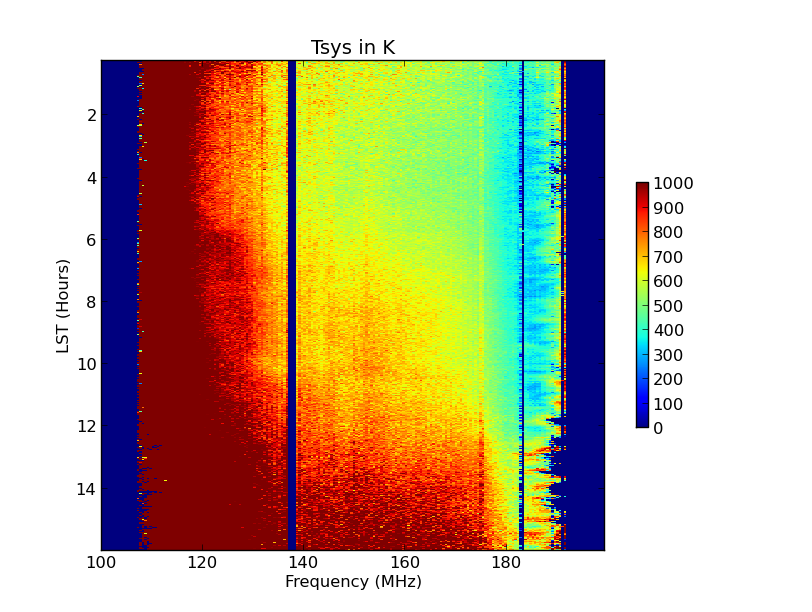
\includegraphics[width=\columnwidth]{plots/tsys_lst_freq.png}
%\caption{Tsys as a function of lst and frequency. The cold spot resides in the
%lst range of 1-7hours.}
%\ref{fig:tsys_lst_fq}
%\end{figure}

\subsection{Fringe-Rate Filtering}\label{sec:frf}
%   -What is fringe rate filtering. Cite Parsons And Liu 2014.
%       --Fringe Rate filtering is nothing more then a time domain weighted
%         average per frequency of of visibilities. The filter can be applied 
%         as either a convolution in the time domain or a multiplicative fourier
%         filter in fringe rate space. 
%       --We first calculate fringe rate filter such that we upweight the more
%         sensitive fringe rates versus the not so sensitve fringe rates by
%         weighting the fringe rates for a given baseline by its beam.
%   -Effective beam areas.
%       --When fringe rate filtering, we are upweighting fringe rates that
%         are most sensitive. That is we are weighting these fringe rates by the
%         beam of a baseline. This has the effect of narrowing the effective
%         beam. It turns out that we are removing more noise than signal,
%         because we are essentially keeping the most sensitive parts of the
%         sky. This actually gives us a sensitivity boost of about a factor of
%         2. 
%   -effective integration time and number of modes. 
%       --Do calculations.
%       --Fringe rate filtering is effectively a weighted average in time and
%       thus there is an effective integration time. We can calculate this
%       integration time by noting that power (or variance) is a conserved
%       quantity. Therefore, comparing the integral of a variance=1 noise signal
%       when it is fringe rate filtered to when it is not, gives us a fractional
%       integration time. 
%           \frac{ \int_{t_{start}}^t_{end}{\sigma^{2}*F_{constant}(t)dt
%           }}{\int_{t_{start}}^t_{end}{\sigma^{2}*F_{filter}(t)dt = fraction.
%            t_int = fraction * t_start-t_end
%           Something like that.
%       --Due to the fact that fringe rate filtering is effectively averaging in
%         time, A fringe rate filter reduces the number of independent modes on
%         the sky. The number of modes in an entire day drop just 45
%         (24hrs/1900sec)  independent modes on the sky. 
%   -PLOTS: 
%       --FR filter (both in fr and time space), applied to data.
%       --Beam after fringe-rate filter. 
%       --Waterfalls.
%       -- apply filters to foreground data. Compute fr of pica and show that we
%          are not killing the sky.
%   
%   code to get the integration time of fringe rate filter. This is 1886 for channel 100
%   beam_w_fr = frf_conv.get_beam_w_fr(aa, (1,4))
%   t,firs,frbins,frspace = frf_conv.get_fringe_rate_kernels(beam_w_fr, 42.8, 401)
%   fr100 = frspace[100]
%   t_int = 42.8/n.mean(fr100)
%   

By averaging visibilities in time, we aim to maximize sensitivity
by coherently combining repeated measurements
of $k$-modes 
before squaring these measurements and averaging over independent $k$-modes
to estimate the power spectrum amplitude.
This is mathematically similar to the more traditional
process of gridding in the $uv$ plane, but applied to a single baseline.
However, rather than applying a traditional box-car average, we can apply a
kernel --- a so-called ``fringe-rate" filter --- that weights different temporal
rates by the antenna beam corresponding to the parts of the sky moving at the
same rate.

For a given baseline and frequency, different parts of the sky
exhibit different fringe-rates.  Maximum fringe rates are found along the
equatorial plane, where the rotation rate of the sky is highest, and zero
fringe rates are found at the poles, where the sky does not rotate and hence
sources do not move through the fringes of a baseline \citep{parsons_backer2009}.
Fringe rates are not constant as a function of latitude. Bins of
constant fringe rate correspond to rings in RA and DEC, where the east-west
projection of a baseline projected toward a patch of the sky is constant.  We
use this fact in conjunction with the root-mean-squared beam response for each
contour of constant fringe rate to construct a time average kernel or
``fringe-rate filter".


%[this paragraph could probably go -dcj]
%As motivation, we discuss the use of fringe-rate filters in cross talk removal.
%Crosstalk is modeled as a time independent coupling of signal between two
%different signal paths. Since crosstalk does not vary as a function of time and shows up at zero fringe rate.  In this view crosstalk is a DC bias. To remove crosstalk, we can
%apply a notch filter to the fringe-rate transform of the time series visibility
%(per frequency) and inverse transform to go back into time domain. This
%interpretation of crosstalk being a DC offset jives with our method of crosstalk
%removal discussed above. In order to remove a DC offset from a time series, we
%subtract the average.
%

As examined in \citet{parsons_et_al2015}, it is possible to tailor fringe-rate filters
to optimally combine time-ordered data for power-spectrum analysis.
Fringe-rate filters can be chosen that
up-weight points of the sky where our instrument is more sensitive and down-weight
those points farther down in the primary beam, which are less sensitive.
For white noise,
all fringe-rate bins will contain the same amount of noise, but the amount of signal
in each bin is determined by the primary beam response on the sky.
By weighting fringe-rate
bins by the root mean square (RMS) of the beam response, we can get a net increase in sensitivity.  
%Upweighting the bins with higher signal relative to those with less signal
%gives us a net increase in signal-to-noise, even though we are removing 
%signal by applying signal from this filter. 

Applying this filter effectively weights the data by another factor of the beam
area, changing the effective primary beam response\footnote{The angular area in
Equation \eqref{eqn:delay_pspec} will reflect the new angular area
corresponding to the change in beam area.}, $A(l,m)$ \citep{parsons_et_al2015}.
By utilizing prior knowledge about the beam area, we are selectively
down-weighting areas on the sky contributing little signal. This will result in
a net improvement in sensitivity depending on the shape of the beam and the
declination of the array. For PAPER, this filter roughly doubles the
sensitivity of our measurements.  

\textbf{Generally, a fringe-rate filter has the property of integrating visibilities. For a 
fringe-rate filter, $f_\text{fr}$, the effective integration time can be calculated by comparing the variance statistic before 
and after filtering. Therefore, the integration time can be calculated as 
\begin{equation}\label{eqn:frf_inttime}
    t_{\text{int,after}} = t_{\text{int,before}}\frac{\int{\sigma^{2}f_{\text{flat}}^{2}df}}{\int{\sigma^{2}f_{\text{fr}}^{2}df}},
\end{equation}
where $t_{\text{int,before}}$ is the integration time before filtering, $\sigma$ is that variance of the signal before filtering, $f_{flat}$ is a flat fringe rate filter and the integral is taken over all possible fringe rates for a given baseline and frequency. As discussed in \citet{parsons_et_al2015}, the
signal loss associated with this fringe-rate filter can be modeled as a modification
of the area of the primary beam.}

\textbf{For the fiducial baseline at a 151 MHz, the integration time, as given in equation \eqref{eqn:frf_inttime}, associated with an optimal fringe rate filter is $3430\, \textrm{s}$. The number of statistically independent samples on the sky decreases from 83 to 1 sample per hour. As discussed in section \ref{sec:sigloss}, empirically estimating a covariance matrix with a small 
number of independent modes can lead to signal loss. In order to counteract the signal loss, we degrade the optimal fringe-rate filter, as seen in figure \ref{fig:fr_preserved_signal}, to have an effective integration time of 1886 seconds, thus increasing the number of independent modes to 2 per hour. Even though the fringe rate filter is now sub-optimal, it holds a big improvement over the boxcar fringe rate weighting as used in P14. As documented in Table \ref{tbl:sigloss}, the correction factor for the associated signal loss of the filter we have chosen is \textbf{1.39}.}

%As a rough check, we note that this is roughly
%the time it takes a source to transit through one fringe period.  Because the
%fringe-rate filter integrates in time, the number of statistically independent
%samples of the sky drastically decreases from 83 to $\sim2$ independent samples
%per hour.

%We implement the optimal fringe-rate filter by calculating the fringe rates at
%every point on the sky, for a given frequency, and weighting each bin by the
%beam of a given baseline. 
%XXX need help describing the actual filter used.
We implement the modified filter on a per baseline basis by weighting the
fringe-rate bins on the sky by the RMS of the beam at that same location.e
In order to obtain a smooth filter in the fringe-rate domain, we fit a Gaussian
with a hyperbolic tangent tail to this filter. In addition, we multiply this
response with another hyperbolic tangent function that effectively zeros out
fringe rates below 0.2 mHz. This removes 
the slowly varying signals that we model as crosstalk. We convolve the
time-domain visibilities with the Fourier transform of the resulting fringe-rate
filter, shown in Figure \ref{fig:fr_preserved_signal}, to produce an averaged
visibility. The effect on the data can be seen in Figure \ref{fig:waterfalls}.

%After LST binning, we apply a fringe-rate filter on a baseline-by-baseline
%basis to remove crosstalk that manifests itself as a slowly varying signal in
%time.  To remove this signal, we apply a fringe-rate filter as a tapered
%hyperbolic tangent function centered at 0.35 millihertz. This effectively
%zeros out fringe rates below 0.2 millihertz, which we attribute to crosstalk.


%\begin{figure}[!t]
%\centering
%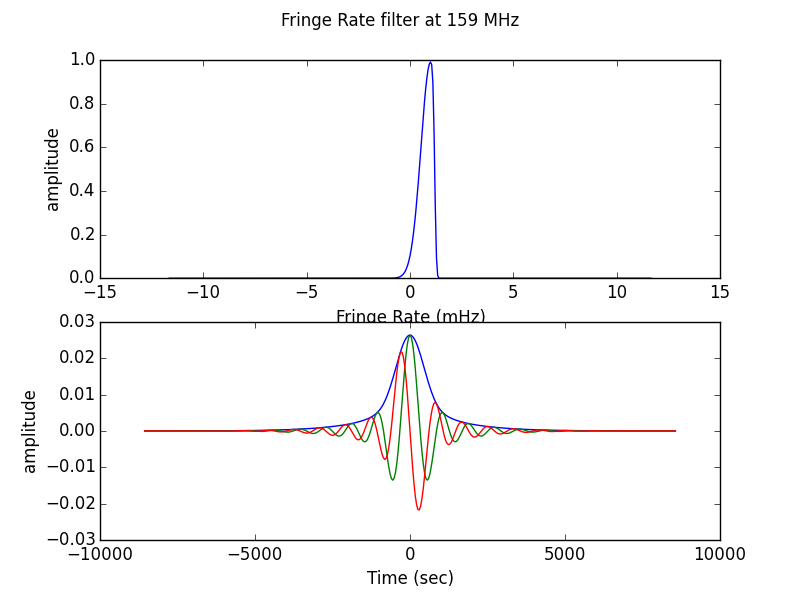
\includegraphics[width=\columnwidth]{plots/fr_filter_slice.png}
%\caption{
%slice of a fringe rate filter at a frequency of 159MHz. Top is the
%filter in fringe rate domain. The bottom consists of the corresponding time
%domain filter gotten by fourier transforming and windowing with a
%blackman-harris window to damp the tails.
%[ move this figure into fringe-rate filter paper]
%}
%\label{fig:fringe_rate_cut}
%\end{figure}

%\begin{figure}\centering
%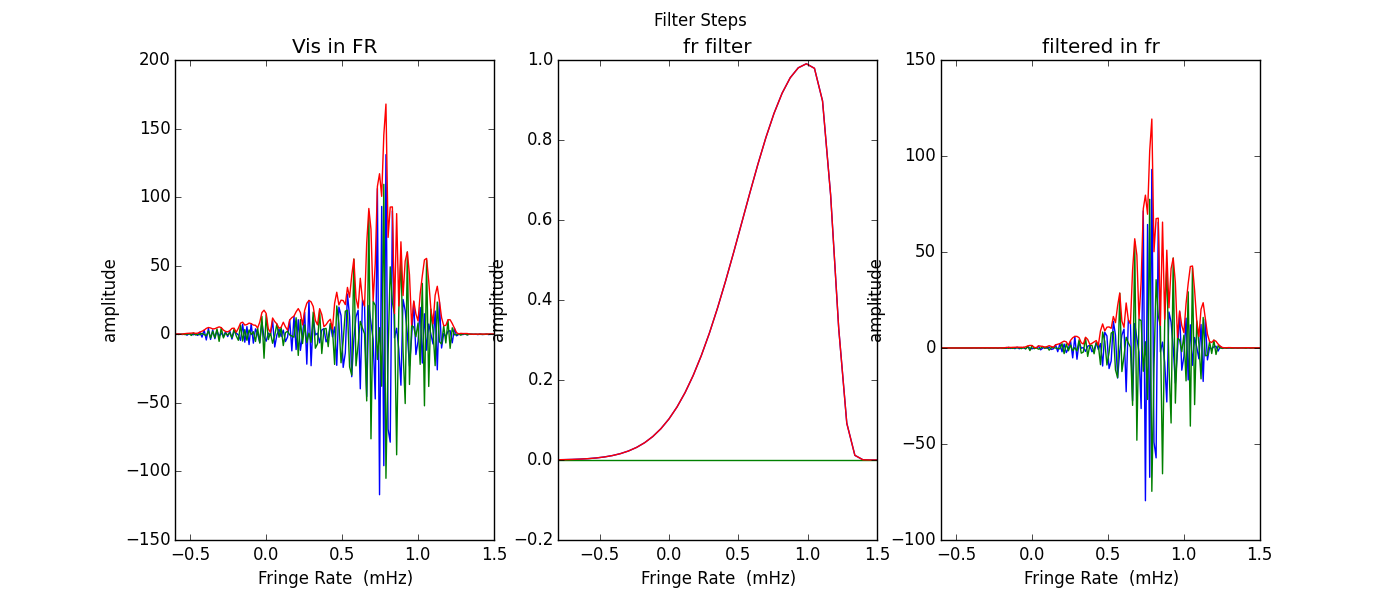
\includegraphics[width=\columnwidth]{plots/fr_preserved_signal.png}
%\caption{
%The magnitude of the fringe-rate transform of foreground contained visibilities measured on the fiducial baseline at 159 MHz before (blue) and after (red) fringe-rate filtering. The fringe-rate filter (green) is normalized to integrate to unity, but has been scaled here for legibility.
%Fringe-rate filtering at 159MHz. Fringe-rates of is defined as the rate at which
%the sky moves through the fringe pattern of a baselines fringe pattern. This is
%dependent on the frequency under consideration as well as position on the sky.
%Shown here is the fringe-rate transform (fourier transform along the time axis
%of a visibility) of unfiltered foreground contained data for a 30 m east-west
%baseline (blue). The fringe-rate filter in fringe-rate space (green) is scaled
%to highlight the shape of the filter. In practice, this filter is normalized so
%that its integral is unity.  This filter is multiplicative in this domain and
%its fourier transform convolves the time domain visibilities from which the
%unfiltered data in this plot is dervied from.  The filtered data (red) is the
%product of the unfiltered with the weights of the fringe-rate filter (green).
%Foreground signal is still retained in the final output, but signal low in the
%beam has been downweighted. For the PAPER array in South Africa, these fringe
%rates correspond to small/negative fringe rates and nearly the maximum fringe
%rates of a 30m east-west baseline. Note the maximum and minimum fringerates
%correspond to the theoretical minimum and maximum for a 30 m baseline at 159
%MHz.
%}
%\label{fig:fr_preserved_signal}
%\end{figure}

\begin{figure}\centering
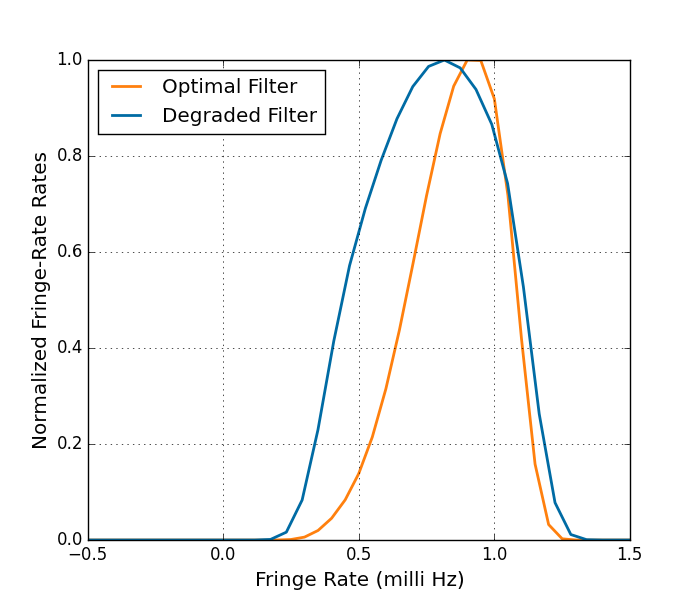
\includegraphics[width=\columnwidth]{plots/fringe_rate_filter.png}
\caption{
The optimal fringe-rate filter (orange) that and the degraded fringe-rate filter (blue) actually used in the analysis  at 151 MHz, normalized to peak at unity. 
%Fringe-rate filtering at 159MHz. Fringe-rates of is defined as the rate at which
%the sky moves through the fringe pattern of a baselines fringe pattern. This is
%dependent on the frequency under consideration as well as position on the sky.
%Shown here is the fringe-rate transform (fourier transform along the time axis
%of a visibility) of unfiltered foreground contained data for a 30 m east-west
%baseline (blue). The fringe-rate filter in fringe-rate space (green) is scaled
%to highlight the shape of the filter. In practice, this filter is normalized so
%that its integral is unity.  This filter is multiplicative in this domain and
%its fourier transform convolves the time domain visibilities from which the
%unfiltered data in this plot is dervied from.  The filtered data (red) is the
%product of the unfiltered with the weights of the fringe-rate filter (green).
%Foreground signal is still retained in the final output, but signal low in the
%beam has been downweighted. For the PAPER array in South Africa, these fringe
%rates correspond to small/negative fringe rates and nearly the maximum fringe
%rates of a 30m east-west baseline. Note the maximum and minimum fringerates
%correspond to the theoretical minimum and maximum for a 30 m baseline at 159
%MHz.
}
\label{fig:fr_preserved_signal}
\end{figure}

%It is important to note that the fringe rate filter is removing some sky signa
%as is seen in figure \ref{fig:waterfalls}, but it is removing 
%The PAPER beam is ~60 degrees FWHM \citep{jacobs_et_al2011}, and the array is
%located at a declination of $-30^{\circ}$ the fringe rates associated with the
%low signal to noise (down in the beam) correspond to very high and very
%low/negative fringe rates.
%%Figure \ref{fig:fringe_rate_cut} shows a cut of the optimal fringe-rate filter
%%at 159 MHz for
%%a 30-m east west baseline. 
%Therefore, the implemented fringe-rate filter removes
%some sky signal, signal associated with fringe rates outside of the ranges shown
%in Figure \ref{fig:fr_preserved_signal}. Figure \ref{fig:fr_preserved_signal} shows
%that the applied filter removes sky associated with negative fringe rates and
%very high fringe rates. [how does this loss compare with the delay spectrum loss?  Can't just leave this statement dangling...]
%

%\begin{figure}[h!]\centering
%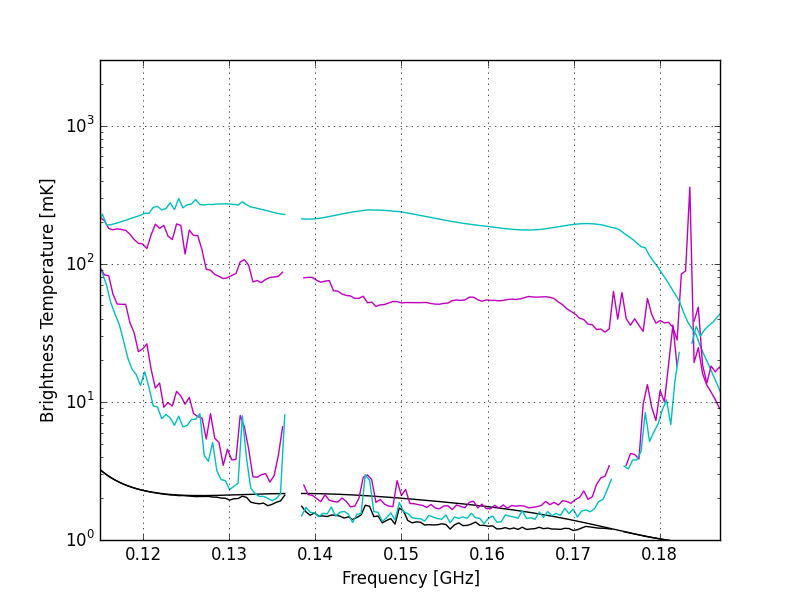
\includegraphics[width=\columnwidth, height=.8\columnwidth]{plots/noise_t_35.png}
%\caption{Estimates of noise temperature. Magenta is frequncy differenced
%estimate where the cyan is the time differenced estimate. All curves are
%averaged over all 30m east-west baselines (56) and averaged incoherently in 43s
%bins of LST from LST 3 to 5 hours with a channel bandwidth of 490 kHz.}
%\label{fig:noise_t}
%\end{figure}


%\begin{figure}[h!]\centering
%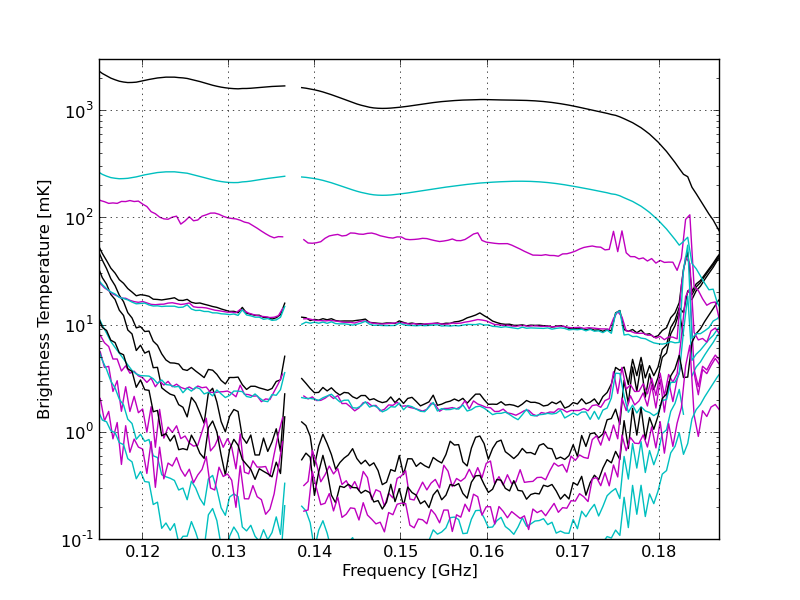
\includegraphics[width=\columnwidth, height=.8\columnwidth]{plots/noise_vs_fq_plot.png}
%\caption{Estimates of noise temperature. Magenta is frequncy differenced
%estimate where the cyan is the time differenced estimate. Averaged in LST from 3
%to 5 hours. on uv files calibrated with omnical. fg,delay filtered, baseline
%averaged, normal fringe rate filter, optimal fringe rate filtering.}
%\label{fig:noise_omni_uv}
%\end{figure}

\section{Instrumental Performance}\label{sec:instrument}
\subsection{Instrument Stability}

\begin{figure*}
\centering
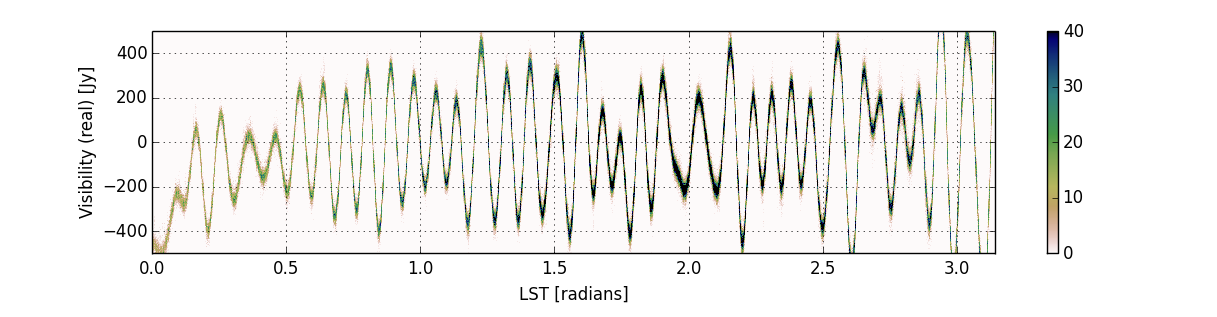
\includegraphics[width=2.3\columnwidth]{plots/density.png}
\caption{Histogram of the real component of all calibrated visibilities
measured over 135 days with every redundant instance of the fiducial baseline at 150
MHz.  Color scale indicates the number of samples falling in an
LST/flux-density bin.  This plot serves to illustrate the stability of the
PAPER instrument and the precision of calibration.  The temporal stability of
a single LST bin over multiple days is shown in Figure \ref{fig:stability}.
%The bulk of the samples recorded, range from an LST of 5 to
%10 hours, whilst the EoR cold spot ranges from 0 to 4 hours as seen in figure
%\ref{fig:coverage}. For the densest regions, the spread in visibility for a
%given LST sample is $\approx{100} \,\text{Jy}$. The agreement between redundant
%baselines here gives us reassurance that our baselines are actually measuring
%the same fourier modes on the sky.}
}\label{fig:density}
\end{figure*}

\begin{figure}
\centering
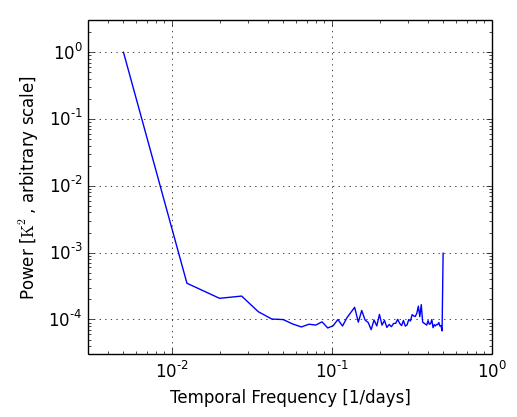
\includegraphics[width=\columnwidth]{plots/stability.png}
\caption{
Power spectrum of 135 days of time-series data contributing to a single LST
bin, illustrating the stability of measurements over the observing campaign.
Relative to the average value, variation in the measured value across days (quantified by
variance as a function of time period) is orders of magnitude lower.
The excess at two-day timescales is a beat frequency associated with
the changing alignment of integration windows in the correlator with respect to
sidereal time. 
%Demonstration of the time stability of the instrument. For a given LST
%bin, we take the day to day samples that go into that bin and determine the
%power spectrum for that time seris. Shown here is the power spectrum of the time
%series over 135 days for baseline 1\_4 at 150 MHz () averaged over 5 hours in
%LST. Power at 1/135 days$^{-1}$ is the DC bin, accumulating the average of the
%time signal. The power spectrum folows a noise like power spectrum throughout
%with a slight uptic at the temporal frequency corresponding to 2 days. This is
%due to the fact that the integration time does not fully divide out a sidereal
%day, but has a remiainder of $\frac{1}{2}$, piling up power on the everyother day
%time scale. ( need to be more clear here, I think. a.const.sidereal\_day/42.9
%= 2008.487, a.const.sidereal\_day/42.94 = 2006.616.)
%}
}\label{fig:stability}
\end{figure}


In order to build sensitivity to the 21~cm reionization signal, it is critical
that PAPER be able to integrate coherently measurements made with different baselines on different days.
Figure \ref{fig:density} shows the visibility repeatability between 
baselines and nights as a function of LST. Specifically, we histogram the real part of
the visibilities for all redundant fiducial baselines 
in a given LST bin for foreground contained data. We see that for a
given LST bin, the spread in values over all the baselines is $\sim$50 Jy which corresponds with our observed
$T_{sys}\sim$500K.  We get
more samples per LST bin in the range of 2--10 hours due to our observing
season, therefore the density of points in this LST region is greater, as shown by
the color scale. This density plot shows that redundant baselines agree very well
with one another; OMNICAL has leveled the antenna gains to within the noise.

Delving in a little deeper, we also examine the
stability in time for measurements in a particular LST bin. In order to quantify the stability
in time we extract one channel for a given baseline for every observation day
and LST bin. We then Fourier transform along the time direction for every LST
bin and compute the power spectrum. As shown in Figure \ref{fig:stability},
for time scales greater than one day, we see that signal variance drops by
almost four orders of magnitude, 
with the exception of an 
excess on two-day timescales caused by the changing alignment of the 42.9~s
integration timescale relative to a sidereal day.  The implication of this
measurement is that, after calibration, PAPER measurements are sufficiently
stable to be integrated coherently over the entire length of a 135-day
observation. This implies day-to-day stability of better than 1\%, contributing
negligibly to the uncertainties in the data.

\subsection{System Temperature}   

During the LST binning step, the variance of the visibilities that are averaged
together for a given frequency and LST bin are recorded. Using these variances,
we calculate the system temperature as a function of LST, averaging over each
LST hour. 
\begin{equation}
    T_{\rm rms} = \Tsys/\sqrt{2\Delta\nu t}, 
\end{equation}
where $\Delta\nu$ is the bandwidth, $t$ is the integration time, and
$T_{\rm rms}$ is the RMS temperature, or the variance statistic described above.
Figure \ref{fig:tsys} shows the results of this calculation. In this observing
season, the system temperature drops just below previous estimates 
as in P14 and \citet{jacobs_et_al2014} of $\Tsys=560\,\textrm{K}$, at
$\Tsys=500\,\textrm{K}$ at 160 MHz. However, this estimate is more consistent
with the results derived in \citep{moore_et_al2015}, where $\Tsys=505K$ at 164
MHz. The change in the system temperature can be attributed to the reduced
range of LST used in the calculation. We note that at 7:00 LST, there is an
increase in the system temperature due to the rising of the galactic plane as
seen in Figure \ref{fig:coverage}.

\begin{figure}\centering
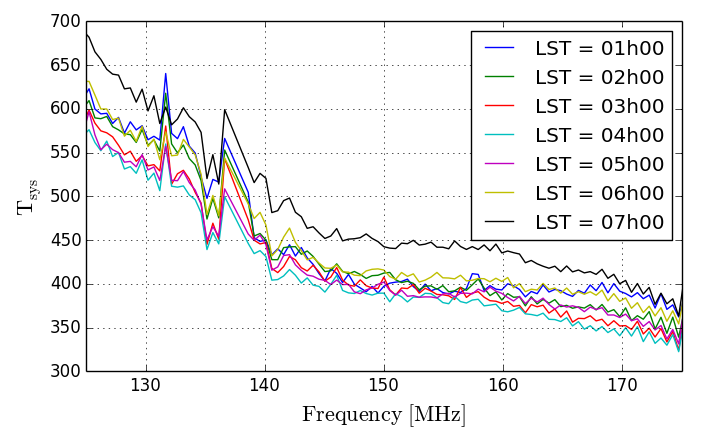
\includegraphics[width=\columnwidth]{plots/tsys.png}
\caption{System temperature, inferred from the variance of samples falling 
in an LST bin, averaged over one-hour intervals in LST.  The measured value
in the 150--160 MHz range is consistent with previous determinations of
system temperature (\citealt{jacobs_et_al2014}; P14).
%statistic calculated in every LST bin and average on hour time scales to
%estimate the $T_{sys}$ reported here. For a majority of the LST bins, especially
%those bins used in our analysis, the system temperature is about 500K at 160
%MHz, consistent with previous estimates of the system temperature.}
}\label{fig:tsys}
\end{figure}

When calculating the system temperature using the variance in the visibilities
for a given LST and frequency, we take into account the fact that we flag
3$\sigma$ outliers from the median. To calculate an effective correction factor
to account for the filtering, we assume the visibilities follow a Gaussian
distribution which would require a correction factor of 1.34 for the removal of
data points that are 3$\sigma$ above the median. In other words, we are
accounting for the wings of the Gaussian that would contribute to the variance
in the visibility.

Previous estimates
of the system temperature
(P14; \citealt{jacobs_et_al2014}) relied on differencing and averaging
baselines, time samples, and/or frequency channels. The relative agreement
between these various methods of estimating the system temperature provides a
robust measure of the system temperature of the PAPER instrument. Agreement
between the instantaneous measurements of the system temperature, the LST
repetition variance, and the predicted power spectrum noise level (see below)
indicates a robustly stable system with no significant long term instability
contributing appreciable noise.



\section{Power Spectrum Analysis}\label{sec:oqe}
%   -Motivate method with discussion of empirical estimate of covariances and
%    problem of limited modes.
%       --Because we dont know the true covariances between baselines and
%         channels we have to estimate the covariances epirically from data. 
%       --We do this by taking the outer product of our data vector (consisting
%         of a visibilies for every baseline of a given unique baseline type).
%         The outer product is calculated per time sample, thus we average over
%         a "clean" (what do i mean by this?) lst range.
%       --Hence, the quality of the estimate of the covariances between
%         baselines depends on the average in time ( the ensemble average). 
%       --The fact that we do not know what the full covariance matrix looks
%         like leads to signal loss. We have an estimate of the covariance, not
%         the true covariance matrix. There is no way to truly know what the
%         covariance matrix is for our data set. 
%       --After fringerate filtering, the number of independent modes on the
%         decreases substantially because we are averaging over 1900 seconds
%         ~=31.67 minutes. Therefore the number of independent modes decreases
%         1900/(the beam in time). 
%       --In our range of lsts used, we only have roughly 20 independent
%         samples. Therefore we end up with an ill determined covariance matrix
%         to describe our data. 
%       --In addition, because of the highly redundant nature of the array,
%         the covariance matrix is highly singular and therefore not invertible.

In this section we first
review the optimal quadratic estimator (OQE) formalism, followed by a walk-through of our 
particular applications of the OQE
method to our data. Finally, we discuss the effects of using an empirically estimated 
covariance matrix in our analysis.



%
%   -Mathematics compared to ideal optimal Quadratic Estimator.
%       --In the quadratic estimator formalism, the value of the power spectrum,
%         $p_{\alpha}$  in the $\alpha^{th}$ bin is given by
%         $Mq_{\alpha}=$Mx^{\dagger}C{-1}Q_{\alpha}C^{-1}x, where x is a vector
%         containing the binned data in frequency domain, $x = V(\nu)$, C is the
%         estimate of the covariance matrix of of our data, C = <xx^{\dagger}>,
%         $Q_{\alpha}$ is defined such that $Q_{\alpha}=\frac{dC}{d\alpha}$, and
%         M is a normalization matrix that normalizes the estimator.
%       --Generally, the covaraince matrix used is the full covaraince between
%         all baselines and channels. 
%       --Because of redundancy, the matrix is singular and not invertible. We
%         therefore construct a pseudo inverse for C. In addtion to the psaudo
%         inverse we take only the auto-baseline covarainces, masking out the
%         covariances between baselines. This, is invertible. WE can thus apply
%         the inverse of C in the above equation.
%
%   -Counting of independent modes.
%       --Number of independent modes = 2*#of lst hours used in analysis. This
%         is because 1900 seconds ~ 30 minutes.
\subsection{Review of Optimal Quadratic Estimators}
We use the optimal quadratic estimator method to estimate our power spectrum as
done in \citet{liu_tegmark2011}, \citet{dillon_et_al2013a}, \citet{liu_et_al2014a}, \citet{liu_et_al2014b}, and \citet{trott_et_al2012}.  Here we briefly review the
optimal quadratic estimator (OQE) formalism with an emphasis on our application
to data, which draws strongly from the aforementioned works, but also relies on empirical
techniques similar to those used in P14. The end goal of this analysis is to estimate the 21 cm
power spectrum, $P_{21}(\k)$, defined such that 
\begin{equation}
\label{eqn:pspec_def}
    \expval{\widetilde{T}_{b}(\k)\widetilde{T}^{*}_{b}(\k^{\prime})} =
            (2\pi)^{3}\delta^{D}(\k - \k^{\prime})P_{21}(\k),
\end{equation}
where $\widetilde{T}_{b}(\k)$ is the spatial Fourier transform of the brightness temperature
distribution on the sky, $\expval{}$ denotes an ensemble average, and
$\delta^{D}$ is the Dirac delta function. 

In order to make an estimate of the power spectrum in the OQE formalism, one begins with a data
vector $\x$. This vector could, for example, consist of a list of brightness temperatures on the sky
for an imaging-based data analysis, or (in our case) a list of measured visibilities. We form
the intermediate quantity,
\begin{equation}
\label{eqn:qalpha}
   \hat{q}_{\alpha} = \frac{1}{2}\x^\dagger\mathbf{C}^{-1}\mathbf{Q}_{\alpha}\mathbf{C}^{-1}\x - b_{\alpha},
\end{equation}
which will be needed to form the optimal quadratic estimator of our power spectrum.
Here, $\mathbf{C} \equiv \langle \x \x^\dagger \rangle$ is the true covariance matrix of the data vector $\x$, 
$\mathbf{Q}_{\alpha}$ is the operator that takes visibilities into power spectrum
$k$-space and bins into the ${\alpha}$th bin, and $b_{\alpha}$ is the bias to
the estimate that needs to be subtracted off. In general, $\mathbf{Q}_{\alpha}$
represents a family of matrices, one for each $k$ bin indexed by $\alpha$. Each matrix
is defined as
$\mathbf{Q}_{\alpha} \equiv
\frac{\partial{\mathbf{C}}}{\partial p_{\alpha}}$, i.e., the derivative of the covariance
matrix with respect to the band power $p_\alpha$. 
%It is important to note that
%$\mathbf{Q}_{\alpha}$ can take on any form and be completely arbitrary. It is
%the data analyst's choice, provided all the relevant
%statistical information (such as the error bars) are self-consistently computed. However, if one is looking for the best possible
%estimate of the power spectrum,  $\mathbf{Q_{\alpha}}$ will typically be
% proportional to  $\mathbf{C}_{,\alpha} \equiv
%\frac{\partial{\mathbf{C}}}{\partial p_{\alpha}}$, defined as the derivative of
%the covariance matrix with respect to the band power $p_{\alpha}$.
The bandpower $p_\alpha$
can be intuitively thought of as the value of the power spectrum in the $\alpha$th
$k$ bin.  Therefore, $\mathbf{Q}_{\alpha}$ encodes the response of the data
covariance matrix to the $\alpha$th bin of the power spectrum. 
%We describe our choice of this
%matrix in the next section, where we describe the application of the quadratic
%estimator. 

The bias term $b_{\alpha}$ in Equation \eqref{eqn:qalpha} will include contributions
from both instrumental noise and residual foregrounds. Their presence in the data
is simply due to the fact that both contributions have positive \emph{power}. One
approach to dealing with these biases is to model them and to subtract them off,
as is suggested by Equation \eqref{eqn:qalpha}. An alternate approach is to
compute a cross-power spectrum between two data sets that are known to have
the same sky signal but independent instrumental noise realizations. Labeling
these two data sets as $\x_1$ and $\x_2$ and computing
%In our analysis, we do not attempt any bias subtraction
%of residual foregrounds. This is a conservative choice motivated by concerns about
%possible signal loss from an overly aggressive bias removal scheme. In any case,
%any residual foreground bias will only serve to raise our upper limit. To deal with the
%instrumental noise bias, we do not apply Equation \eqref{eqn:qalpha} as written. Doing
%so would constitute the computation of an auto-power spectrum, where data---and thus
%instrumental noise contributions---are squared, causing a positive bias. Instead, we
%split the data $\x$ into two groups $\x_1$ and $\x_2$, which are comprised of visibilities
%from different copies of a redundant baseline in the array. If one then computes
\begin{equation}\label{eqn:qalpha_unbiased}
    \hat{q}_{\alpha} =
\frac{1}{2}\x_{1}^\dagger\mathbf{C}^{-1}\mathbf{Q}_{\alpha}\mathbf{C}^{-1}\x_{2},
\end{equation}
one arrives at a cross-power spectrum that by construction has no noise bias. There is
thus no need to explicitly model and subtract any noise bias, although any residual foreground
bias will remain, since it is a contribution that is sourced by signals on the sky, and therefore
must exist in all our data sets.

The set of $\hat{q}_{\alpha}$s do not yet constitute a properly normalized estimate of
the power spectrum (as evidenced, for example, by the extra factors of $\mathbf{C}^{-1}$). 
To normalize our results, we group the unnormalized bandpowers into a vector $\mathbf{\hat{q}}$
and apply a matrix $\mathbf{M}$ (whose exact form we specify later), so that
\begin{equation}\label{eqn:pspec_norm}
    \mathbf{\hat{p}} = \mathbf{M}\hat{\mathbf{q}}
\end{equation}
is a normalized estimate $\mathbf{\hat{p}}$ of the true power spectrum $\mathbf{p}$. We emphasize
that the vector space that contains $\hat{\mathbf{q}}$ and $\hat{\mathbf{p}}$ is an ``output" vector
space over different $k$-bins, which is separate from the ``input" vector space of the measurements, in which $\x$ and $\mathbf{C}$ reside.

To select an $\mathbf{M}$ matrix that properly normalizes the power spectrum, we must compute
the window function matrix $\mathbf{W}$ for our estimator. The window matrix is defined such that
the true bandpowers $\mathbf{p}$ and our estimates $\hat{\mathbf{p}}$ of them are related by
\begin{equation}\label{eqn:true_pspec_2_est_pspec}
\hat{\mathbf{p}} = \mathbf{W} \mathbf{p},
\end{equation}
so that each row gives the linear combination of the true power that is probed by our estimate. With
a little algebra, one can show that 
\begin{equation}\label{eqn:window_def}
    \mathbf{W} = \mathbf{M}\mathbf{F}, 
\end{equation}
where
\begin{equation}
\label{eq:FisherMatrix}
\mathbf{F}_{\alpha\beta} =
\frac{1}{2}\textrm{tr}(\mathbf{C}^{-1}\mathbf{Q}_{\alpha}\mathbf{C}^{-1}\mathbf{Q}_{\beta}),
\end{equation}
which we have suggestively denoted with the symbol $\mathbf{F}$ to highlight the fact that this turns out to be the Fisher
information matrix of the bandpowers. In order to interpret each bandpower as the weighted
average of the true bandpowers, we require each row of the window function matrix to sum to
unity. As long as $\mathbf{M}$ is chosen in such a way that $\mathbf{W}$ satisfies this criterion, the resulting bandpower estimates
$\hat{\mathbf{p}}$ will be properly normalized.

%$\mathbf{F}$ is the Fisher information matrix, given by
%
%and $\mathbf{W}$ is the window function matrix. The window functions measure the
%degree to which power from $k$ bins couple into the measurement of the power
%measured in the $\alpha$'th $k$ bin. Specifically, 
%\begin{equation}\label{eqn:true_pspec_2_est_pspec}
%    \hat{\mathbf{p}} = \mathbf{W}\mathbf{p}, 
%\end{equation}
%where $\mathbf{p}$ and $\hat{\mathbf{p}}$ are vectors of the true power spectrum and our
%estimate of the power spectrum for every $\alpha$'th bin, respectively. Note
%that the window functions are normalized such that the rows of $\mathbf{W}$ sum
%to unity.

%   -Cholesky Decomposition and window functions.
%       --The optimal window functions (that minimize the vertical error bars of
%       the estimate, are given by the inverse of the Fisher matrix. However,
%       there is a trade off such that this incorporates information from all of
%       the k-modes. 
%       --Some other choices of the window functions are the square root of the
%       fisher matrix or the identity. 
%       --We use the cholesky decomposition of the Fisher Matrix such that we
%       can write F = LL^{\dagger}, where L is a lower triangular matrix. This
%       is possible for any hermitian positive-definite matrix.
%       --We use L for our window functions because for every k-bin, it does not
%       use information from the k-bins below it. And thus there is no mixing of
%       modes lower than it. 
%       --This is particularly important because it doesn't insures that there
%       is no leakage of the modes within the horizon to modes outside of it.         
%
Beyond the normalization criterion, a data analyst has some freedom over the
precise form of $\mathbf{M}$, which effectively also re-bins the bandpower estimates. One 
popular choice is $\mathbf{M} = \mathbf{F}^{-1}$, which implies that $\mathbf{W} = \mathbf{I}$. Each
window function is then a delta function, such that bandpowers do not
contain leakage from other bins, and contain power from only that bin. However, the disadvantage
of this becomes apparent if one also computes the error bars on the bandpower estimates.
The error bars are obtained by taking the square root of the diagonal of the covariance matrix, which is defined as
\begin{equation}\label{eqn:err_cov}
    \boldsymbol \Sigma = \text{Cov}(\hat{\mathbf{p}}) = \expval{\hat{\mathbf{p}}\hat{\mathbf{p}}^{\dagger}} -
             \expval{\hat{\mathbf{p}}}\expval{\hat{\mathbf{p}}}^{\dagger}.
\end{equation}
Since $\phat = \mathbf{M}\qhat$, it is easily shown that 
\begin{equation}
\label{eq:MFM}
  \boldsymbol  \Sigma = \mathbf{M}\mathbf{F}\mathbf{M}^{\dagger}.
\end{equation}
The choice of $\mathbf{M} = \mathbf{F}^{-1}$ tends to give rather large error bars.
At the other extreme, picking $\mathbf{M}_{\alpha \beta} \propto \delta_{\alpha \beta} / \mathbf{F}_{\alpha \alpha}$ (with the proportionality constant fixed by our normalization criterion) 
leads to the smallest possible error bars \citep{tegmark1997}, at the expense of broader
window functions. In our application of OQEs in the following sections, we will pick an intermediate
choice for $\mathbf{M}$, one that is carefully tailored to avoid the leakage of foreground power
from low $k$ modes to high $k$ modes.

%
%In addition to calculating the window functions, we can also calculate the error
%correlations that correspond to a given window function. In order to see the
%effect of the normalization matrix on the error correlations we start by looking
%at the covariance of the band power estimates, namely, 
%\begin{equation}\label{eqn:err_cov}
%    \boldsymbol \Sigma = \text{Cov}(\hat{\mathbf{p}}) = \expval{\hat{\mathbf{p}}\hat{\mathbf{p}^{\dagger}}} -
%             \expval{\hat{\mathbf{p}}}\expval{\hat{\mathbf{p}}}^{\dagger}.
%\end{equation}
%Since $\phat = \mathbf{M}\qhat$, it is easily shown that 
%\begin{equation}
%    \Sigma = \mathbf{M}\mathbf{F}\mathbf{M}^{\dagger},
%\end{equation}
%where $\mathbf{F}$ is the Fisher matrix. The error correlation matrix describes
%how correlated the errors between modes are in the final power spectrum result.


\subsection{Application of Optimal Quadratic Estimators}
\label{sec:oqe_app}
% A walk through of the application to the data.

Here we describe the specifics of our application of the optimal quadratic
estimator formalism to measure the power spectrum. Doing so requires defining
various quantities such as $\x$, $\mathbf{C}$, $\mathbf{Q}_\alpha$ for our analysis
pipeline.

First, we consider $\x$, which represents the data in our experiment.  Our data set consists
of visibilities as a function of frequency and time for each baseline in the
array. In our analysis, we group the baselines into three groups of redundant baselines (described in
Section \ref{sec:observations}), 
in the sense that within each group there are multiple copies of the same baseline. In the
description that follows, we first estimate the power spectrum separately for each group.
Power spectrum estimates obtained from the different redundant groups are then combined in a set of averaging and bootstrapping steps described in Section \ref{sec:bootstrap}. Note that because
our data have been fringe-rate filtered in the manner described in Section \ref{sec:frf},
we may reap all the benefits of coherently integrating in time simply by estimating the power spectrum
for every instant in the LST-binned data before averaging over the time-steps within the LST-binned day \citep{parsons_et_al2015}.

For the next portion of our discussion, consider only the data within a single redundant group. Within each group there are not only multiple identical copies of the same baseline, but in addition (as discussed in
Section \ref{sec:wbd_filtering}), our pipeline also constructs two LST-binned data sets, one from binning all even-numbered days in our observations, and the other from all odd-numbered days. Thus, 
we have not a single data vector, but a whole family of them, indexed by baseline ($i$) and odd
versus even days ($r$). Separating the data out into independent subgroups allows one to estimate
cross-power spectra rather than auto-power spectra in order to avoid the noise bias, as discussed in the previous section. The data vectors take the form
\begin{equation}
\label{eqn:xvectdef}
\mathbf{x}^{ri}(t) = \left( \begin{array}{c}
V^{ri} (\nu_1, t) \\
V^{ri} (\nu_2, t) \\
\vdots \\
\end{array}
\right), 
\end{equation}
where $V^{ri} (\nu, t)$ is the visibility at frequency $\nu$ at time $t$. Each data vector is 
20 elements long, being comprised of 20 channels of a visibility spectrum spanning $10\,\textrm{MHz}$ of bandwidth centered on $151.5\,\textrm{MHz}$.
%
%Focusing on the fiducial
%baselines, our data vector becomes a list of visibilities
%such that
%\begin{equation}
%\label{eqn:xvectdef}
%\mathbf{x} = \left( \begin{array}{c}
%V (t_{1}) \\
%V (t_{2}) \\
%\vdots \\
%\end{array}
%\right), 
%\end{equation}
%where, $V(t_{i})$ is the visibility of a baseline, indexed by LST bin,
%belonging to the redundant baselines under consideration. Each visibility
%contains 10 MHz of bandwidth centered at 151.5 MHz, amounting to 20 channels. 
%Notice that we have only included data from one baseline, which is looking ahead
%to the application of the method our data. We in effect apply the quadratic
%estimator on a per baseline basis and sum the baselines together to get our
%final estimate. The important point is that the data vector is in frequency
%space, where our final power spectrum estimate is in Fourier space. 

Having formed the data vectors, the next step in Equation \eqref{eqn:qalpha} is to
weight the data by their inverse covariance. To do so, we of course require the covariance
matrix $\mathbf{C}$, which by definition, is the ensemble average of
$\x\x^\dagger$, namely $\mathbf{C} = \expval{\x\x^\dagger}$. Unfortunately, in our case the
covariance is difficult to model from first principles, and we must resort to an
empirically estimated $\mathbf{C}$. We make this estimation by taking the time average
of the quantity $\x\x^\dagger$ over 8.5 hours of LST, estimating a different covariance matrix
for each baseline and for odd versus even days. While an empirical determination of the covariance is advantageous
in that it captures features that are difficult to model from first principles, it
carries the risk of cosmological signal loss \citep{switzer_liu2014}. We will discuss and quantify this signal loss
in Section \ref{sec:sigloss}.

To gain some intuition for the action of $\mathbf{C}^{-1}$ on our data, let us examine the
combination
\begin{equation}\label{eqn:z}
    \mathbf{z}^{ri} =  (\mathbf{C}^{ri})^{-1}\mathbf{x}^{ri}
\end{equation}
for select baselines. This is a crucial
step in the analysis since it suppresses coherent frequency structures (such as those
that might arise from residual foregrounds). Note that the inverse covariance weighting employed
here differs from that in P14, in that P14 modeled and included covariances between
different baselines, whereas in our current treatment we only consider covariances between
different frequency channels. 
Figure \ref{fig:inv_cov} compares the effects of applying
the inverse covariance matrix to a data vector that contains foregrounds (and thus contains
highly correlated frequency structures) to one in which foregrounds have been suppressed
by the wideband
delay filter described in Section \ref{sec:wbd_filtering}. In the figure, the
top row corresponds to the data vector $\mathbf{x}^{ri}$ for three selected baselines in the form
of a waterfall plot of
visibilities, with frequency on the horizontal axis and time on the vertical axis. The
middle section shows the empirical estimate of the covariance by taking the
outer product of $\x$ with itself and averaging over the time axis. Finally,
the last row shows the results of inverse covariance weighting the data,
namely $\mathbf{z}^{ri}$. In every row, the foreground-dominated data are shown
in the left half of the figure, while the foreground-suppressed data are shown in the right half.

Consider the foreground-dominated $\mathbf{x}^{ri}$ in Figure \ref{fig:inv_cov}, and
their corresponding covariance matrices. The strongest modes that are present in the
data are the eigenmodes of the covariance matrix with the largest eigenvalues. Figure
\ref{fig:eigs} shows the full eigenvalue spectrum and the four strongest eigenmodes.
For the foreground-dominated data, one sees that the eigenvalue spectrum is dominated
by the first few modes, and the corresponding eigenmodes are rather smooth, highly suggestive
of smooth spectrum foreground sources. The application of the inverse covariance weighting
down-weights these eigenmodes, revealing waterfall plots in the bottom row of Figure \ref{fig:inv_cov}
that look more noise-dominated. With the foreground-suppressed portion (right half) of Figure \ref{fig:inv_cov},
the initial $\mathbf{x}^{ri}$ vectors already appear noise dominated (which is corroborated by the
relatively noisy form of the eigenvalue spectra in Figure \ref{fig:eigs}). The final $\mathbf{z}^{ri}$ vectors
remain noise-like, although some smooth structure (perhaps from residual foregrounds) has still been removed, and finer scale noise
has been up-weighted.

\begin{figure*}\centering
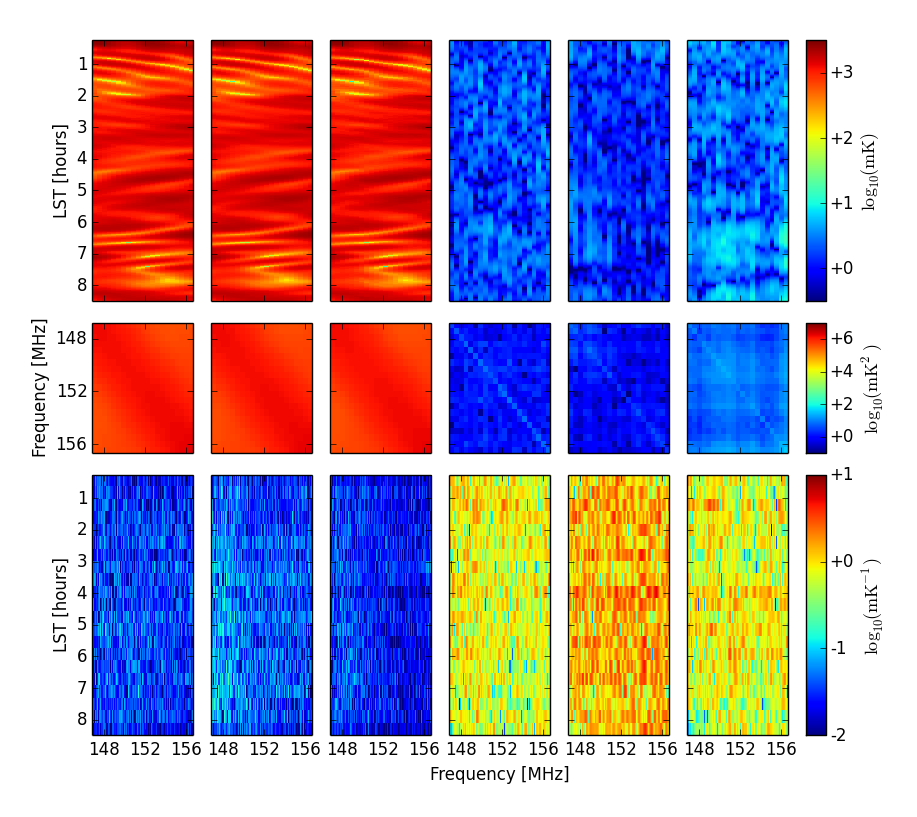
\includegraphics[width=2\columnwidth]{plots/inv_cov.png}
\caption{
Visibilities before (top row) and after (bottom row) inverse covariance weighting.
Signal covariance (middle row) is estimated empirically, averaging over LST.
The three left/right columns show visibilities from
three different baselines in a redundant group before/after delay filtering, respectively.
} \label{fig:inv_cov}
\end{figure*}

\begin{figure}\centering
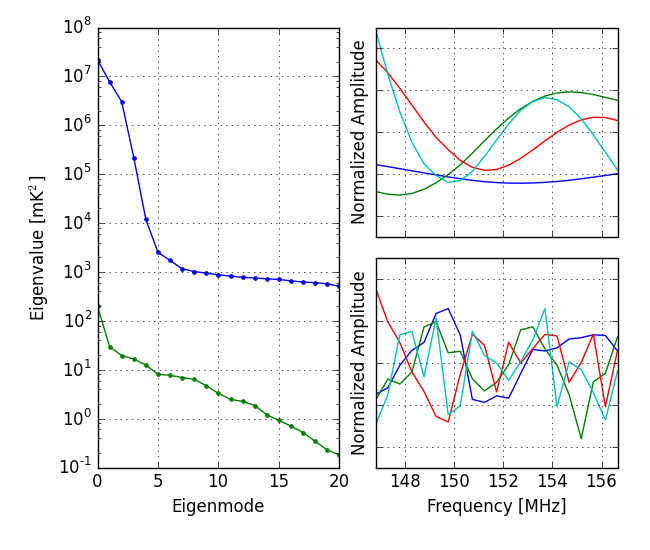
\includegraphics[width=\columnwidth]{plots/eig.png}
\caption{
Eigenvalue spectrum of covariance matrices (left) empirically estimated 
from visibilities before (blue) and after (green) delay filtering.
The four strongest eigenmodes of the filtered/unfiltered data are plotted
on the top/bottom panels on the right, respectively.
%The eigenspectrum for the foreground contained data
%has a sharp decline for the first few eigen modes and levels of at around 1 K,
%suggesting that most of the variation in the data are only described by a
%handfull of eigenmodes. The four strongest corresponding eigenmodes (top right
%panel) shows that these modes are smooth spectrum modes, suggestive of smooth
%foregrounds.  Contrastingly, the eigenspectrum for delay filtered data, in which
%foregrounds are heavily filtered, steadily decreases suggesting that there are
%not a few modes that mostly describe all of the variation in the data. This is
%paralleled in the strongest eigenmodes for this filtered data (bottom right
%panel) and there is no coherent structure to any of these modes. 
} \label{fig:eigs}
\end{figure}


With intuition established for the behavior of $\mathbf{C}^{-1}$, we may group our identical
baselines into five different sets and average together $\mathbf{z}^{ri}$ vectors for baselines
within the same set. That is, we form
\begin{equation}\label{eqn:presum_oqe}
    \mathbf{z}^{r}_{A} = \sum_{i\in{A}} (\mathbf{C}^{ri})^{-1}\mathbf{x}^{ri},
\end{equation}
where $A$ ranges from $1$ to $5$ and indexes the baseline set. At this point,
we have 10 weighted data vectors $\mathbf{z}$ ($5$ baseline sets, each of which has
an even day and odd day version) for every LST-binned time-step. As discussed in the
previous section, instrumental noise bias may be avoided by forming cross-power spectra
rather than auto-power spectra. Generalizing Equation \eqref{eqn:qalpha_unbiased} to our
present case where we have $10$ different data vectors, we have
\begin{equation}\label{eqn:presum_qalpha}
    \qhat_{\alpha} = \sum_{\substack{A,B,r,s\\r\ne{s},A\ne{B}}}\mathbf{z}^{r\dagger}_{A}\mathbf{Q}_{\alpha}\mathbf{z}^{s}_{B},
\end{equation}
so that auto-power contributions from identical baseline groups or identical even/odd indices
never appear. Residual foreground bias will remain in Equation \eqref{eqn:presum_qalpha}, 
but in order to avoid possible signal loss from an overly aggressive foreground bias removal scheme, 
we conservatively allow the foreground bias to remain. Since foreground power will necessarily
be positive, residual foregrounds will only serve to raise our final upper limits.

In order to implement Equation $\eqref{eqn:presum_qalpha}$, it is necessary to derive a form for
$\mathbf{Q}_\alpha \equiv \partial \mathbf{C} / \partial p_\alpha$. To do so, we follow the delay
spectrum technique of P12a, where it was shown that
\begin{equation}\label{eqn:delay_pspec}
    P(\mathbf{k}_{t\tau}) \approx
\Big(\frac{\lambda^{2}}{2k_{B}}\Big)^{2}\frac{X^{2}Y}{\Omega
B}\expval{\tilde{V}_{i}(t,\tau)\tilde{V}_{j}^{*}(t,\tau)},
\end{equation}
where $V_{i}(t,\tau)$ is the delay transform of baseline visibilities given by Equation \eqref{eqn:delay_transform}, $X$ and
$Y$ are the constants that convert from angles and frequency to the co-moving
coordinate, respectively, $\Omega$ is the power squared beam (see Appendix B of
P14), $B$ is the bandwidth, $\lambda$ is the spectral wavelength, and $k_{B}$ is Boltzmann's constant.
This suggests that in order to estimate the power spectrum from visibilities, one only needs
to Fourier transform along the frequency axis (converting the spectrum into a delay spectrum)
before squaring and multiplying by a scalar. Thus, the role of $\mathbf{Q}_\alpha$ in Equation \eqref{eqn:presum_qalpha} is to perform a frequency Fourier transform on each copy of
$\mathbf{z}$. It is therefore a separable matrix of the form $\Q_{\alpha} =
\mathbf{m}_{\alpha}\mathbf{m}_{\alpha}^{\dagger}$, where $\mathbf{m}_{\alpha}$ is a
complex sinusoid of a specific frequency corresponding to delay mode $\alpha$.
%[I can make this more rigorous, but it'll require a few more lines of math. Zaki, your call. ARP: not worth the trouble]
%This
%separable form holds only for short baselines, where the chromaticity of an interferometer
%can be neglected over narrow bandwidths [cite wedge paper 1]. Fortunately, as discussed
%above [right?], only short baselines are used in our analysis here, and we may thus
% ARP: the above caveat relates to the interpretation of delay modes as k modes, but doesn't apply to constructing a delay-mode estimator
We may thus write
\begin{equation}
    \qhat_{\alpha} =
\sum_{\substack{A,B,r,s\\r\ne{s},A\ne{B}}}\mathbf{z}^{r\dagger}_{A}\mathbf{m}_{\alpha}\mathbf{m}_{\alpha}^{\dagger} \mathbf{z}^{s}_{B}.
\end{equation}
With an explicit form for $\mathbf{Q}_\alpha$, one now also has the necessary ingredients
to compute the Fisher matrix using Equation \eqref{eq:FisherMatrix}.

Having computed the $\qhat_{\alpha}$s, we group our results into a vector $\mathbf{\hat{q}}$.
This vector of unnormalized bandpowers is then normalized to form our final estimates of the
power spectrum $\mathbf{p}$. As noted above, the
normalization occurs by the $\mathbf{M}$ matrix in Equation
\eqref{eqn:pspec_norm}, and can be any matrix of our desire. 
Even though the choices of the normalization matrices described above have certain
good properties, e.g. small error bars or no leakage, we opt for a different
choice of window function, as follows. We first reorder the elements in $\mathbf{\hat{q}}$ (and
therefore in $\mathbf{F}$, $\mathbf{M}$, and $\mathbf{\hat{p}}$ for consistency) so that
the $k$-modes are listed in ascending order, from low $k$ to high $k$, with the exception that we place the highest $k$ bin third after the lowest two $k$ bins. (The reason for this exception will be made apparent shortly). We then take the Cholesky decomposition of
the Fisher matrix, such that $\mathbf{F}=\mathbf{L}\mathbf{L}^{\dagger}$, where
$\mathbf{L}$ is a lower triangular matrix. Following that, we pick ${\mathbf{M}} = \mathbf{D} \mathbf{L}^{-1}$, where $\mathbf{D}$ is a diagonal matrix chosen to adhere to the normalization constraint
that $\mathbf{W} = \mathbf{M} \mathbf{F}$ has rows that sum to unity. In this case, the window function matrix becomes,
$\mathbf{W}=\mathbf{D} \mathbf{L}^{\dagger}$. This means that $\mathbf{W}$ is upper triangular,
and with our ordering scheme, has the consequence of allowing power to leak from high to low $k$,
but not vice versa. Since our $k$ axis is (to a good approximation) proportional to the delay axis, foregrounds preferentially appear at low $k$ because their spectra are smooth. Reducing leakage
from low $k$ to high $k$ thus mitigates leakage
of foregrounds into the cleaner, more noise-dominated regions. Additionally, our placement of the highest $k$ bin as the third element in our reordering of 
$\mathbf{\hat{p}}$ prevents leakage from this edge bin that will contain aliased power. Figure
\ref{fig:window_func} shows the resulting window functions. 

\begin{figure}\centering
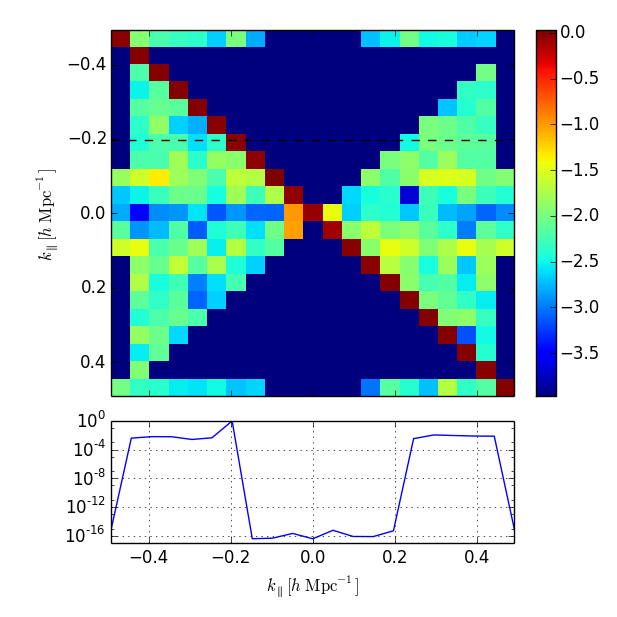
\includegraphics[width=\columnwidth]{plots/window.png}
\caption{
The window function matrix $\mathbf{W}$, as defined in Equation \eqref{eqn:true_pspec_2_est_pspec}.
The $i^{\rm th}$ row corresponds to the window function
used in the estimate of the power spectrum for the $i^{\rm th}$ $k$-mode.
Color scale indicates $\log_{10}\mathbf{W}$.
The inset plot illustrates the window function along the dashed line in the upper panel.
As described in Section \ref{sec:oqe_app}, $\mathbf{M}$ in Equation \eqref{eqn:window_def} has been chosen so that
each window function peaks at the waveband while achieving a high degree of isolation from
at lower $k$-modes that are likely to be biased by foregrounds.
}\label{fig:window_func}
\end{figure}

Our choice of normalization matrix also has the attractive property of eliminating error correlations
between bandpower estimates. Using Equation \eqref{eq:MFM}, we have
that \begin{equation} 
 \boldsymbol   \Sigma = \mathbf{D} \mathbf{L}^{-1}\mathbf{L}\mathbf{L}^{\dagger}\mathbf{L}^{-\dagger} \mathbf{D}
           = \mathbf{D}^2.
\end{equation}
The error covariance matrix on the bandpowers is thus diagonal, which implies
that our final data points are uncorrelated with one another. This stands in contrast to the power-spectrum estimator used in P14, where the Blackmann-Harris taper function induced correlated errors
between neighboring data points.



\subsection{Covariance Matrix and Signal Loss}
\label{sec:sigloss}
%Covariance matrix nuances.
%   -describe covariance matrix and data vectors.
%   -How we get the covariance matrix. 
%   -eigenvalue decomposition.
%mode counting and nonsingular-ness.
%   -Count independent modes.
%   -covaraiance is independent only if we have enough indendent modes.
%   -inverse covariance is tricky because of this. 
%   -happy coincidence?
%

We now discuss some of the subtleties associated with empirically estimating the covariance matrix from
the data. Again, the covariance matrix is defined as the ensemble average of the outer
product of a vector with itself, i.e., 
\begin{equation}
    \C = \expval{\x\x^{\dagger}}, 
\end{equation}
where $\x$ is the data (column) vector used in the analysis. In our analysis,
we do not have \emph{a priori} knowledge of the covariance matrix. and thus we
must resort to empirical estimates \citep{dillon_et_al2015}. As we have alluded to above, we replace
the ensemble average with a time average that runs from 0 to 8:30 LST hours.

Since the OQE method for power spectrum estimation requires the inversion
of $\C$, it is crucial that our empirically estimated covariance be a full rank matrix.
With our data consisting of visibilities over $20$ frequency channels, the covariance
matrix is a $20 \times 20$ matrix. Thus, a necessary condition for our estimate to be
full rank is for there to be at least $20$ independent time samples in our average. As noted in Section \ref{sec:frf} the fringe-rate filter used corresponds to averaging time samples for 31 minutes. Over the LST range
used in this analysis, this corresponds to roughly 20 statistically
independent modes in our data after fringe-rate filtering. We therefore have just enough
samples for our empirical estimate, and in practice, our covariance matrices are invertible
and allow OQE techniques to be implemented.

%The optimal quadratic estimator has an application of the inverse covariance
%matrix to data vector $\x$. Applying an inverse covariance matrix to the data it
%is derived from has the effect of weighting the data by the covariance matrix.
%Therefore strong modes, corresponding to the eigenvectors of the covariance
%matrix, are down-weighted in this scheme as seen in Figure \ref{fig:inv_cov}.
%For foreground contained data, the strong modes correspond to the smooth
%spectrum foregrounds, and therefore the covariance matrix is highly covariance
%since all of the frequency channels are correlated with one another. However,
%for foreground filtered data, the strongest modes correspond to modes that
%resemble residual foreground in the data. It is important to note that inverse
%covariance weighting is a powerful tool as seen by looking at the three
%baselines used in Figure \ref{fig:inv_cov}. For the baseline data vector with
%the least amount of noise in the delay filtered plot (right half, middle
%column), we can see that weighing by the inverse covariance up-weights modes in
%this baseline, as compared to the other baselines, which have a slightly higher
%noise in the original data vector. This is even paralleled in the foreground
%contained data.
%
%   -Potential for signal loss.
%       --In a traditional OQE method, the process is lossless by construction.
%         Because we are tweaking this method, and the fact that we have non
%         Gaussian systematics in our data, there is a potential for signal
%         loss. 


Another potential problem that occurs from empirically estimating covariances is that it
leads to models of the covariance matrix that over-fit the noise. In this
scenario, the covariance matrix tells us that there may be modes in the data
that should be down-weighted, for example, but if the empirical covariance estimates are dominated
by noise, these may just be random fluctuations that need not be down-weighted. Said differently, the weighting of the data by the inverse
covariance is heavily influenced by the noise in the estimate of the covariance
matrix and thus has the ability to down-weight valid high-variance samples. 
%In order to accurately describe the covariance matrix of our measurements, we would require complete knowledge of the sky signal and the instrument and the interaction of the two due to the chromaticity of the interferometer.
Over-fitting the noise in this manner carries with it the possibility of cosmological signal loss.
This seems to contradict the conventionally recognized feature of OQEs as
lossless estimators of the power spectrum \citep{tegmark1997}. However,
the standard proofs of this property assume that statistics such as $\mathbf{C}$
are known \emph{a priori}, which is an assumption that we are violating with our
empirical estimates.
%
%
%In theory, optimal quadratic estimators for the power spectrum described above are a
%lossless operation. However, this requires that we have all the information
%needed to accurately estimate the power spectrum. One of the biggest
%uncertainties, as noted above, is the lack of a perfect covariance matrix that
%describes all of the covariances of the sky and instrument, which can lead to
%signal loss in the final estimate of the power spectrum.  In order to quantify the amount of signal loss we can get by empirically estimating the covariances, we describe the simulations and report on the signal loss we expect with our estimates.


%   -Simulations
%       --In order to show the degree that there could be signal loss, we run
%         simulations to show that an EOR -like signal does pop come out in our
%         data. 
%       --We inject a common eor like signal, a complex random white noise
%         signal, on to all of the baseline data used in this analysisi for a
%         given time. This signal is fringe rate filtered to match the data and
%         therefore, the number of independent modes matches the input data. 
%       --We run this simulation for varying signal levels, showing that this
%         signal can infact be recovered, with some signal loss.
%       --These simulations show that there is signal loss in this method.
%         However, if the signal was bright enough, we would be able to see it.
%         Since we don't see signal in the actual data, we can say that we have
%         not detected the EOR signal yet.

\begin{figure}
\centering
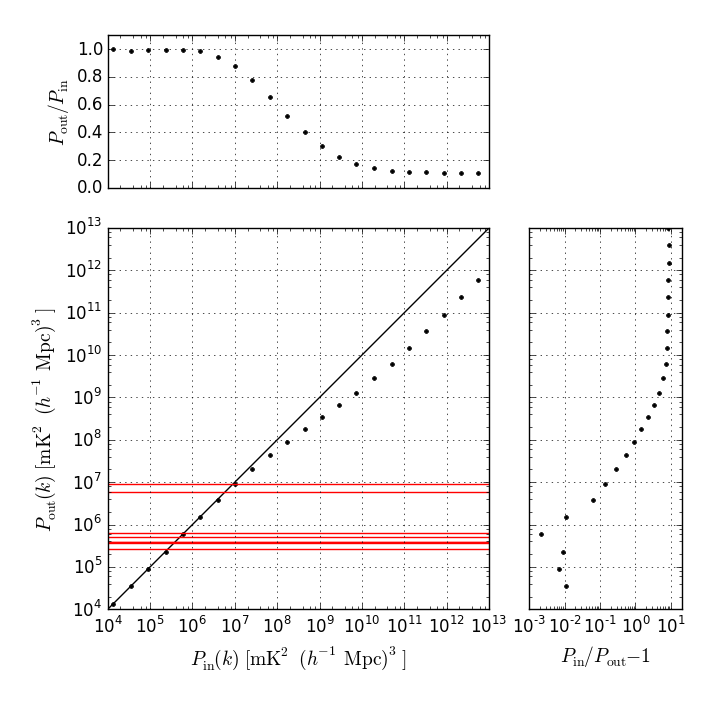
\includegraphics[width=\columnwidth]{plots/sigloss.png}
\caption{
Recovered power spectrum signal as a function of injected signal amplitude.  Shaded regions
indicate the range in measured amplitude of power spectrum modes in Figure \ref{fig:final_pspec}.  
Error bars indicate 95\% confidence intervals as determined from the Monte Carlo simulations
described in Section \ref{sec:sigloss}.
Because
the recovered signal amplitude is a monotonic function of the injected signal amplitude,
it is possible to invert the effects of signal loss in the measured power spectrum values
to infer the true signal amplitude on the sky. Over the range of powers measured, the 
maximum correction factor $P_{\rm in}/P_{\rm out}$ is less than 1.02 at 97.5\% confidence.
The transition to significantly higher correction factors at larger signal amplitudes
occurs as the injected signal
dominates over the foreground modes present in estimates of the data covariance.
}\label{fig:signal_loss}
\end{figure}

In order to deal with possible signal loss, we perform simulations of our analysis pipeline, 
deriving correction factors that must be applied to our final constraints. We simulate visibilities for
Gaussian temperature field with a flat amplitude in $P(k)$ that rotates with the
sky, which is fringe-rate filtered in the same way as the data for our fiducial baselines. This signal is processed through our pipeline, and the output power spectrum compared to the input
power spectrum, for various levels of input signal amplitude.
We repeat this for 40 sky realizations at each signal level.  Figure
\ref{fig:signal_loss} shows the resultant signal loss associated with
estimating the covariance matrix from the data.  Error bars were obtained
through bootstrapping.

As a function of the increasing input amplitude of the simulated power spectra,
we find that the ratio of output power to input power decreases, which we interpret
 as signal loss through the use of our empirical OQE of the power spectrum.  
However, since the transfer function through this analysis is an invertible function,
we can correct for the transfer by using the output value to infer a signal loss
that is then divided out to obtain the original input signal level.  In Figure \ref{fig:signal_loss},
we see that
deviations from unity signal transfer begin at
power spectrum amplitudes of $10^{7} \text{mK}^{2} (h^{-1}\rm
\,\text{Mpc})^{3}$. For the range of output power spectrum amplitudes in our
final estimate of the 21 cm power spectrum (Figure \ref{fig:final_pspec}), we
show that signal loss is $<2\%$ at $95\%$ confidence. 

\begin{table}[htdp]
\caption{SIGNAL LOSS VERSUS ANALYSIS STAGE}
\begin{center}
\begin{tabular}{rll}
Analysis Stage & Typical Loss & Maximum Loss \\
\hline
Bandpass Calibration &  $< 2 \times 10^{-7}\%$ & 3.0\% \\
Delay Filtering & $1.5\times10^{-3}\%$ & 4.8\% \\
Fringe-rate Filtering & 28.1\% & 28.1\% \\
Quadratic Estimator & $<2.0\%$ & 89.0\% \\
Median of Modes & 30.7\% & 30.7\% \\
\end{tabular}
\end{center}
\label{tbl:sigloss}
\end{table}%

As shown in Table \ref{tbl:sigloss}, the signal loss we characterize for quadratic
estimation of the power spectrum band powers is tabulated along with the signal
loss associated with each other potentially lossy analysis stage (see Figure \ref{fig:flowchart}).
We correct for the signal loss in each stage by multiplying the final power spectrum results
by the typical loss for each stage, except for modes within the horizon limit and immediately
adjacent to the horizon limit, where we apply the maximum signal loss correction to be conservative.

% Carina's Text of the eor model goes here.  Will put in on revision
%The model eor signal used was a simulation of a flat power spectrum, in P($k$),
%from $k$-modes ranging from .1-10 $\text{hMpc}^{-1}$. From this an angular power
%spectrum is computed (\cite{datta_et_al2007, lewis_challinor_2007}), ensuring
%correlation in frequency/redshift for the power spectrum maps. Visibilities are
%then simulated for this power spectrum map by explicitly integrating fringes on
%the sky every 42.8 seconds for an East-West baselin of 30 m.

%In order to effectively characterize signal loss in our analysis pipeline, we
%simulate visibilities that accurately capture the instrumental effects of PAPER
%for the frequency bins used in the analysis. The signal injected into the
%simulation is comprised of two components - an artificial power spectrum P(k)
%and frequency extrapolated galactic foregrounds from the Global Sky Model (GSM)
%(de Oliveira-Costa et al. 2008). The injected power spectrum is flat in P(k) for
%a k-range of 0.1-10 $\text{hMpc}^{-1}$, and the angular power spectrum is computed from
%this (\cite{datta_et_al2007, lewis_challinor_2007}), ensuring correlation in
%frequency/redshift for the power spectrum maps. PAPER visibilities are simulated
%for both the GSM and power spectrum maps by explicitly integrating fringes on
%the sky every 42.8s for an East-West baseline of 30m.


%Need to argue that the detections are not Gaussian and therefore are not eor
%detections.


%   -Maybe : Problem of low noise measurements in this method of analysis i.e.
%    singular matrics - For Adrian.
%
%   -Boot strapping 
%       --In order to calculate the residual noise in our power spectrum
%         estimate, we bootstrap the baseline samples at the output of the
%         quadratic estimator. 
%       --Doing this gives us the variance of the power spectrum estimate and
%         thus derives the 2 sigma error bars shown in the power spectrum. 
%       --We are careful to not incur a noise bias by making sure that the
%         groups used do not contain the same baselines. However, the pull from
%         each group is random with replacement. Each group can have a repeat of
%         a baseline. 
%       --We use 100 bootstraps to derive our error bars, setting a $2\sigma$
%         bound on the errors.

\subsection{Bootstrapped Averaging and Errors}\label{sec:bootstrap}

\begin{figure*}\centering
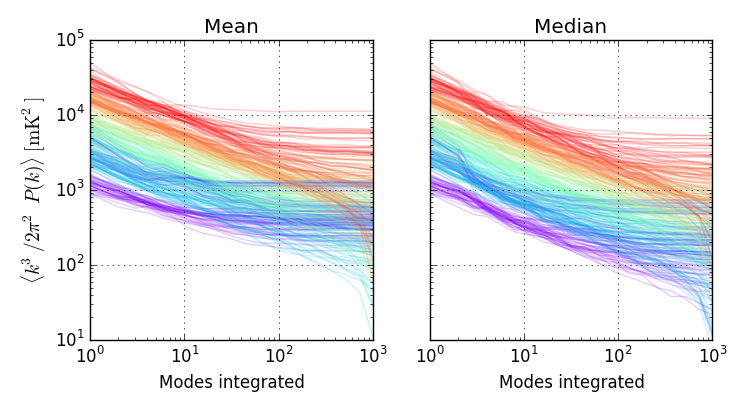
\includegraphics[width=1.8\columnwidth]{plots/pspec_variance.png}
\caption{
Absolute value of the cumulative mean (left) and median (right), as a function of number of modes 
of the power spectrum band power for
$k_\parallel$ modes ranging from $-0.49$ (red) to $0.44\hMpci$ (violet).
Here, modes are defined as samples from different redundant baseline groups and LSTs.
This Allen variance plot shows modes averaging down as the square root of
number of modes combined until a signal floor is reached.  The difference in
behavior between the mean and median is an indication of outliers
in the distribution of values, likely as a result of foreground contamination.
We use the median in the estimation of the power spectrum in Figure \ref{fig:final_pspec},
along with a correction factor compensating for the difference between the mean and median
in estimating variance.
}\label{fig:pspec_variance}
\end{figure*}


When estimating our power spectra via optimal quadratic estimators, we generate
multiple samples of the power spectrum in order to apply the bootstrap method to
calculate our error bars. In detail, the power spectrum estimation scheme proposed
above requires averaging at several points in the pipeline:
\begin{itemize}
\item Visibilities are averaged into five baseline groups after inverse covariance weighting (see Equation \eqref{eqn:presum_oqe})
\item Power spectrum estimates from each of the three redundant baseline types (described in Section \ref{sec:observations}) are averaged together.
\item Power spectrum estimates from each LST are averaged together.
\end{itemize}
With the bootstrapping technique, we do not directly perform these averages. Instead,
one draws random samples within the three-dimensional parameter space specified above,
with replacement, until one has as many random samples as there are total number of parameter
space points. These random samples are then propagated through the power spectrum pipeline
and averaged together as though they were the original data. This forms a single estimate (a ``bootstrap") of $P(\mathbf{k})$. Repeating 
random draws allows one to quantify the inherent scatter---and hence the error bars---in our
estimate of $P(\mathbf{k})$. When plotting $\Delta^2 (k) \equiv k^3 P(k) / 2 \pi^2$ instead of
$P(\mathbf{k})$, we bin power falling in $+k$ and $-k$, and so 
we additionally randomize the inclusion of 
positive and negative $k$ bins.

We compute a total of 400 bootstraps. In combining independent samples for our final power spectrum
estimate, we elect to use the median, rather than the mean, of the samples. One can see the behavior 
of both statistics in Figure \ref{fig:pspec_variance}, where we
show how the absolute value of $\Delta^2(k)$ integrates down as more independent samples are included in the mean and median.
In this plot, one can see modes integrating down 
consistent with a noise-dominated power spectrum until they bottom out on a signal.
In the noise-dominated regime, the mean and the median
behave similarly.  However, we see that the median routinely continues to integrate down as noise for longer.
This is an indication that the mean is skewed by outlier modes, suggesting variations beyond thermal noise. The magnitude of the difference
is also not consistent with the Rayleigh distribution expected of a cosmological power spectrum limited by cosmic
variance.  
For a Rayleigh distribution, the median is $\ln2 \sim 0.69$ times the mean. 
Instead, we interpret the discrepancy as a sign of contributions from foregrounds, which are neither isotropic 
nor Gaussian distributed.  Since median provides 
better rejection of outliers in the distribution that might arise from residual foreground power, we choose to use
the median statistic to combine measurements across multiple modes.
As listed in Table \ref{tbl:sigloss}, we apply a $1/\ln2$ correction factor to our power spectrum estimates to 
infer the mean from the median of a Rayleigh distribution.


%When applying this method of estimating the
%statistical variance in our data, we require that there needs to be a random
%component in our estimates of power spectra.
%
%We use the baseline axis as our random draw axis. For each bootstrap we
%calculate the power spectrum of a random draw of $N_{bls}-5$, giving us more
%than $2\times10^6$ possible combinations of baselines for the fiducial
%baselines used in the analysis and over $1\times10^{6}$ combinations of the 
%redundant baseline groups used in the analysis.
%There is enough variation in
%the data to tease out the underlying statistics of the distribution. 
%
%There are, however, a few issues that must be dealt with in order to not incur a
%noise bias that will. We want to effectively construct an unbiased estimator.
%There are two ways that our estimate of the power spectrum can incur a noise
%bias as discussed earlier. One way is to have an auto cross multiplication in
%the quadratic estimator. We avoid this by only using cross baseline products
%when estimating the power spectrum as discussed above. And furthermore, we use
%the cross products in both time and baselines, as described above.

%In our analysis we use 100 bootstraps, to calculate the error bars as a function
%of $k$-mode in our final power spectrum. In the calculation of the error bars,
%we randomly sample 400 samples from the 100 bootstraps to measure the $1
%\text{and} 2 \sigma$ errors. One key point here is that we use the median
%statistic in order to measure the variance in our power spectrum, rather than
%the mean statistic. This is due to the fact that there are outliers that
%drastically skew the final error bars. 


%
%Figure \ref{fig:pspec_variance} shows that the mean and variance statistic used
%in the estimate of the band powers have similar properties. Namely, some modes
%integrate down and bottom out on a signal with the addition of more samples.
%However, there are a few modes that show a bottoming out, but take a dive when
%more modes are added, owning to some peculiar noise properties in the
%measurements. Generally, the two statistics have similar properties. Assuming
%Gaussian statistics; they should be the same. However, there is a correction factor that needs to be applied to
%the measured power spectrum because we are not in the completely noise dominated
%regime, due to the fact that there are clear detections. Therefore, for these
%modes we are in a Rayleigh distributed regime, in which the mean and median are
%not equal. The correction factor is $\log{(2)}$ for using the
%median statistic over the mean, for a Rayleigh distributed signal. Noting that
%we are somewhere in-between these two distributions, as implied by the fact that 
%some of our error bars are consistent with zero and some are clear detections.
%We therefore apply this correction factor as an upper bound on the discrepancy
%of using these two statistical metrics.


%\subsubsection{Integrating $k$-modes}
% This shows the efficacy of using the median over the mean.
%The power spectrum shown in figure \ref{fig:final_pspec} is an average of
%multiple baselines together. To show how the modes in each power spectrum
%integrate together and to what degree they integrate down as noise are not, an
%allan variance test, is shown in Figure \ref{fig:pspec_variance}. Color
%represents a different $k$ mode measured in $\Delta^{2}$ along with the
%different bootstraps. Here we are showing the effect of integrating down on
%different $k$ modes as we include a wider range in time, and hence more
%independent modes. From the discussion on optimal fringe rate filtering we know
%we have 2 independent modes on the sky per LST hour. Hence, integrating modes
%upto a thousand modes, where not all are independent we expect to hit up against
%a floor, which we see. These curves are plotted for $P(k)$ and therefore, the
%colors represent both positive and negative $k$'s with green curves haveing the
%highest absolute value for $k$ and blue curves are modes closer to the horizon.
%
%
%We see a slight difference in the mean and median statistic when estimating the
%total value of modes. Modes tend to level off for both the statistcs and the
%amount of independent modes is capped when modes flatten out at roughly ~60
%samples. We find that this is close to the number of independent modes on the
%sky and baselines. In addtion modes close to the horizon (blue) tend to flatten
%out with the mean statictic, however there is an increased spread for the median
%statistic. 
%
%In addtion there is a sharp decline in power when integrating ~1024 modes for
%certain modes when dealing with the mean and median statistic. These modes show
%unexpected behaviour due to the sharp slope of the fall in power. Further
%investigation of these modes is to be conducted.
%


%
%   -PLOTS:
%       --example covariance matrices (with foregrounds, without, fringe rate
%         filtering.
%       --Before and After covariance application waterfall plots.
%
%       --Eigen Spectra and shape of the eigen modes.
%
%       --Window Functions : not waterfalls.
%
%       --Fisher matrices.
%
%       --Power spectrum waterfall plots for different separations. 
%
%       --Maybe the wedge.
%



%\section{Summary of Improvements from PSA32}
% Should this section be here? [ARP: no, it is now in discussion]
%In comparison to the previous PAPER pipeline (see \cite{parsons_et_al2014a}),
%this analysis took a slightly different approach which included some critical
%steps to improve our upper limit. In short, the improvements included using a
%new, refined redundant calibration method (Zheng 2014), increasing the width of
%the wideband delay filter that removes smooth spectrum foregrounds, weighting
%the lst binned data sets, and optimal fringe rate filtering. In section
%\ref{sec:calib}, we dicuss each of the improvements in more detail.
%
%Figure \ref{fig:step_through_pspec} (TBD) shows the power spectra when each of
%the steps mentioned above are turned off and for the one where all of them are
%turned on. We can see the gradual improvement of the power spectra (hopefully).


%%%%%%%%%%%%%%%%%%%%%%%%%%%%%%%%%%%%%%%%%%%%%%%%%%%%%%%%%%%%%%%%%%%%%%%%%%%%%%%%%%%


\section{Results}\label{sec:results}

\subsection{Power Spectrum Constraints}
To summarize the previous section, we follow 
the power spectrum analysis procedure outlined in Section \ref{sec:oqe_app},
we incoherently combine independent power spectrum measurements made at different
times and with different baseline groups using the median statistic.  As described
in Section \ref{sec:bootstrap}, we bootstrap over all of these independent measurements,
as well as over the selection of baselines included in the power spectrum analysis for
each baseline group, in order to estimate the error bars on the spherically averaged
power spectrum $P(k)$, where positive and negative $k_\parallel$ measurements
are kept separate for diagnostic purposes.  In the estimation of the 
dimensionless power spectrum
$\Delta^{2}(k)\equiv{k^{3}P(k)}/{2\pi^{2}}$, the folding of $\pm k_\parallel$ is
handled along with the rest of the bootstrapping over independent modes.
Finally, the measured values for $P(k)$ and $\Delta^2(k)$ are corrected for signal
loss through all stages of analysis, as summarized in Table \ref{tbl:sigloss}.

\begin{figure*}\centering
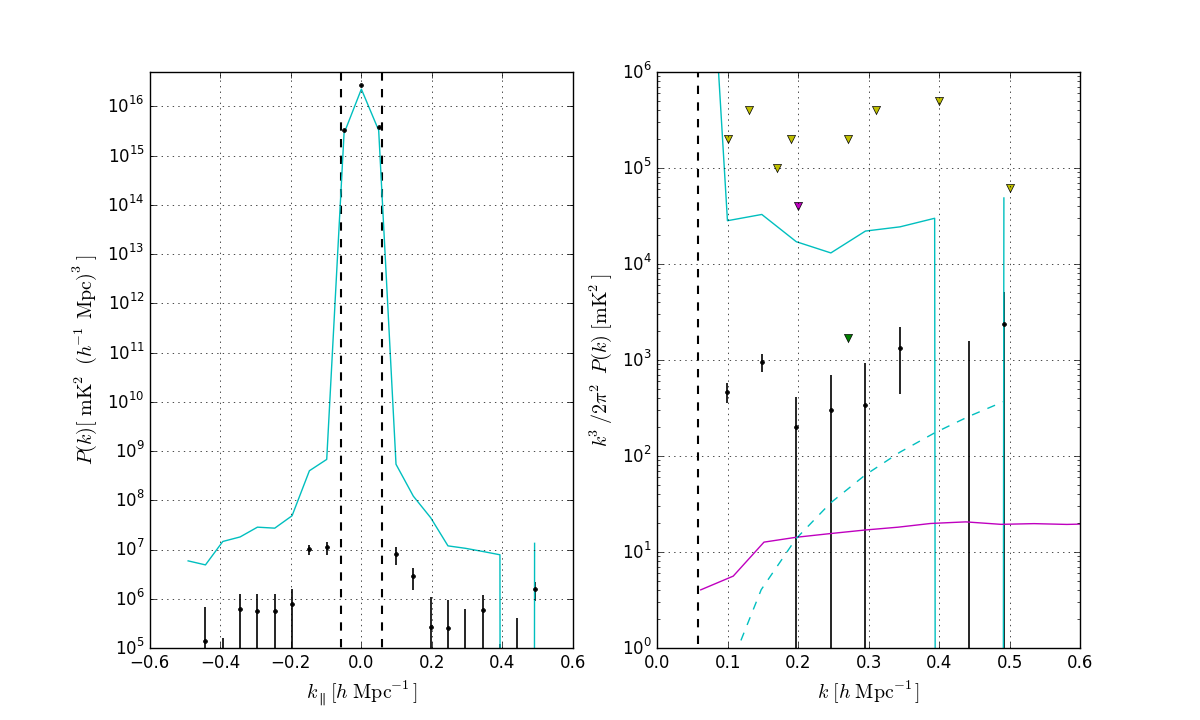
\includegraphics[width=2\columnwidth]{plots/pk_k3pk.png}
\caption{
Measured power spectrum (black dots with 2$\sigma$ error bars) at $z=8.4$
resulting from a 135-day observation with PAPER-64.  The dashed vertical lines
at $0.6\hMpci$ show the bounds of the delay filter described in Section
\ref{sec:wbd_filtering}. The predicted 2$\sigma$ upper limit in the absence of the a celestial signal is shown in dashed cyan, assuming $\Tsys=500K$. The triangles indicate 2
$\sigma$ upper limits from GMRT \citep{paciga_et_al2011} (yellow) at $z=8.6$,
MWA \citep{dillon_et_al2013b} at $z=9.5$ (magenta), and the previous PAPER upper
limit (P14) at $z=7.7$ (green). The magenta curve shows a predicted model 21 cm power
spectrum at 50\% ionization \citep{lidz_et_al2008}.
} \label{fig:final_pspec}
\end{figure*}

The final results are plotted in Figure \ref{fig:final_pspec}.
For the first two modes outside of the horizon where $\Delta^2(k)$ is measured, we have
clear detections. We attribute these to foreground leakage from
inside the horizon related to the convolution kernels in Equation \eqref{eqn:delay_transform} (either
from the chromaticity of the antenna response, or from the inherent spectrum of the
foregrounds themselves).  Somewhat more difficult to interpret are the 
$2.4\sigma$ excess at $k\approx0.30\hMpci$ and 
the $2.9\sigma$ excess at $k\approx0.44\hMpci$. Having two such outliers is
unlikely to be chance.

\begin{figure*}\centering
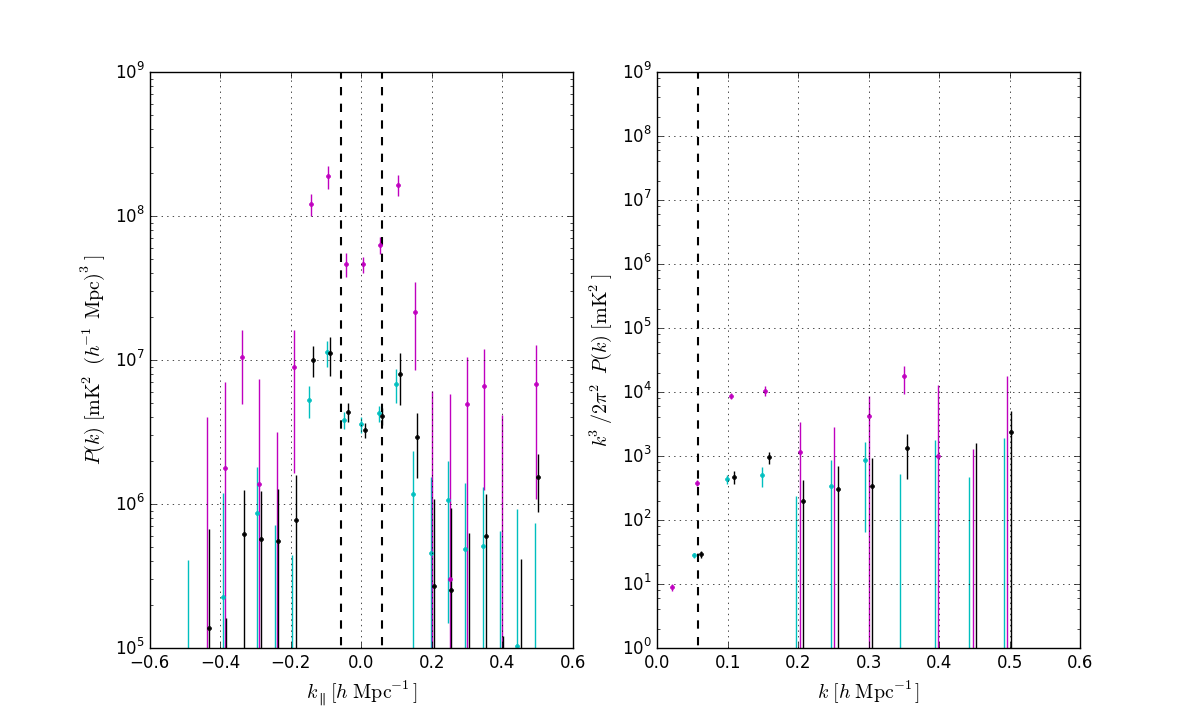
\includegraphics[width=2\columnwidth]{plots/pspec_comparison.png}
\caption{
Diagnostic power spectra in the style of Figure \ref{fig:final_pspec}
illustrating the impact of various analysis stages.
The blue power spectrum uses the P14 fringe-rate filter combined with crosstalk removal.
Green illustrates the result using the improved fringe-rate filter, but without crosstalk removal.
A power spectrum derived without the application of OMNICAL is shown in orange.  Black
includes improved fringe-rate filtering, crosstalk removal, and OMNICAL calibration; it is the 
same power spectrum shown in Figure \ref{fig:final_pspec}.
}\label{fig:pspec_comp}
\end{figure*}


In examining the effects on the power
spectrum of omitting various stages of analysis (see Figure \ref{fig:pspec_comp}), we
see a pronounced excess in the green curve corresponding 
to the omission of crosstalk removal in fringe-rate filtering.
While the signal is heavily attenuated in the filtering step, it remains a
possibility that the remaining detections are associated with instrumental crosstalk.
We do note, however, that the qualitative shape of the excess in the crosstalk-removed data
does not appear to match that of the crosstalk-containing data.

Another likely possibility is that the signal might be associated with foregrounds.
Foregrounds, which are not generally isotropically distributed on the sky, are likely
to be affected by the spatial filtering associated with fringe-rate filtering, whereas
a statistically isotropic signal is not.  
Indeed, we see that excesses in many modes
measured with using the P14-stype time-domain filtering (blue in Figure \ref{fig:pspec_comp})
decrease significantly using the improved fringe-rate filter.  
As discussed in \citet{parsons_et_al2015},
the normalization applied to $\Omega_{\rm eff}$ for fringe-rate filtering correctly
compensates for the effect of this filtering on power-spectral measurements
of a statistically isotropic Gaussian sky signal.  We can surmise from any significant change in amplitude of the excess
under fringe-rate filtering that it arises from emission that violates these assumptions.
We conclude, therefore, that this excess is unlikely to be cosmic reionization, and is more
likely the result of non-Gaussian foregrounds.
As discussed earlier, one possible
culprit is polarization leakage \citep{moore_et_al2013,jelic_et_al2010,jelic_et_al2014}, although further
work will be necessary to confirm this.  The interpretation of
the signal as polarization leakage is, however, rather high to be consistent
with recent measurements in Stokes Q presented in \citet{moore_et_al2015},
where the leakage is constrained to be $<$ 100 mK$^{2}$ for all $k$.

That the
excesses at $k\approx0.30$ and 0.44$\hMpci$ are relatively unaffected by the filtering
could be an indication that they are more isotropically distributed, but more likely, it
may mean that the simply arise closer to the center of the primary beam where they are
down-weighted less.
Both excesses appear to be significantly affected by omitting OMNICAL calibration
(orange in Figure \ref{fig:pspec_comp}).  This could be interpreted as indicating the 
excess is a modulation induced by frequency structure
in the calibration solution.  However, OMNICAL is constrained
to prohibit structure common to all baselines, so a more likely interpretation is that 
this faint feature decorrelates without the precision of redundant calibration.  To
determine the nature of these particular excesses, further work will be necessary.

\begin{figure}\centering
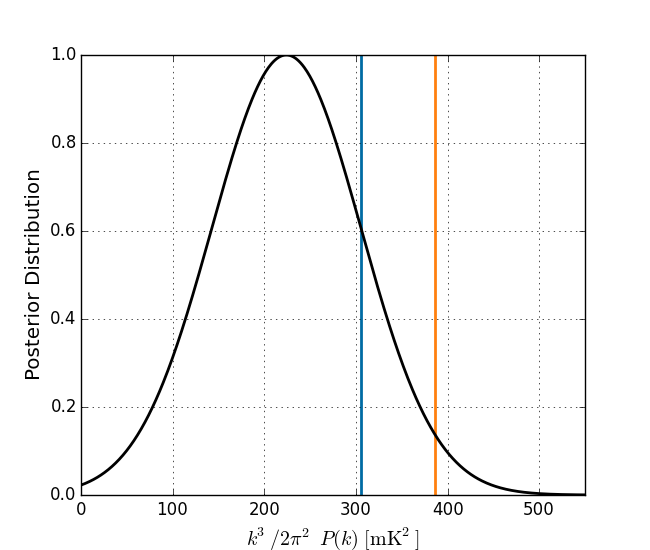
\includegraphics[width=\columnwidth]{plots/flat_k3pk_posterior.png}
\caption{
Posterior distribution of power spectrum amplitude for a flat $\Delta^{2}(k)$
power spectrum over $0.15<k<0.5\hMpci$ (solid black),
assuming Gaussian error bars. The blue and orange
vertical lines correspond to the 1$\sigma$ and 2$\sigma$ bounds, respectively.
%The posterior distribution excluding the the detection at $k=.35\rm \,hMpc^{-1}$ (dashed black) is shown for comparison.
}
\label{fig:final_posterior}
\end{figure}

In order to aggregate the information presented in the power spectrum into
a single upper limit, we fit a flat $\Delta^2(k)$ model to measurements
in the range $0.15<k<0.5\hMpci$.  We use a uniform prior of amplitudes between
-5000 and 5000 ${\rm mK}^2$, and assume measurement errors are Gaussian.
Figure \ref{fig:final_posterior} shows the posterior distribution of the fit.
From this distribution, we determine a mean of
(18.9 mK)$^2$ and a $2\sigma$ upper limit of \mKlimit.
The measured mean is inconsistent with zero at the 4.7$\sigma$ level, indicating that
we are detecting a clear power spectrum excess at $k>0.15\hMpci$.

We suspect that the excess in our measured power spectrum is likely caused
by crosstalk and foregrounds.  We therefore suggest ignoring the lower bound on the power spectrum amplitude
as not being of relevance for the cosmological signal.  On the other hand, since foreground
power is necessarily positive, the 
2$\sigma$ upper limit of \mKlimit at $z=8.4$, continues to serve as a conservative upper limit. This significantly improves over the previous
best upper limit of $(41~{\rm mK})^2$ at $z=7.7$ reported in P14.
As we show below and in
greater detail in \citet{pober_et_al2015}, this limit begins to have implications
for the heating of the intergalactic medium prior to the completion of reionization.

\subsection{Spin Temperature Constraints}

\begin{figure*}\centering
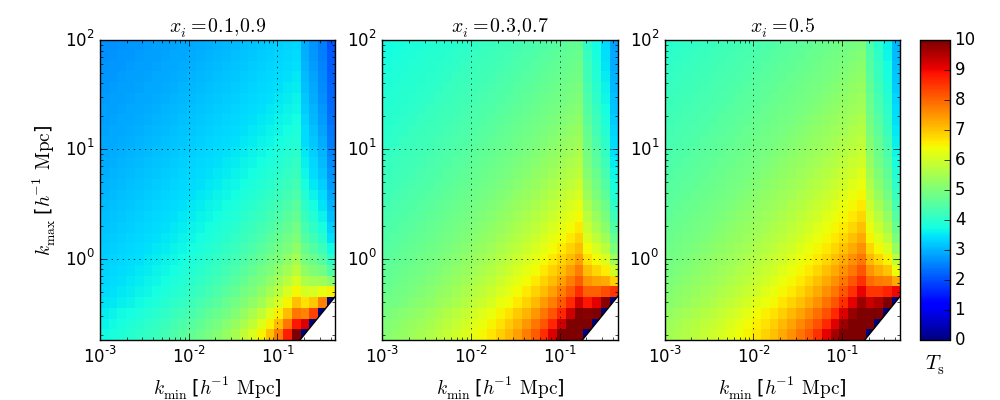
\includegraphics[width=2\columnwidth]{plots/ts_patchy_bound.png}
\caption{Constraints on the 21cm spin temperature at $z=8.4$, 
assuming 
the patchy reionization model in Equations
\eqref{eqn:d2pspec_model} and \eqref{eqn:patchy_bound}, which hold in the limit
that $T_{\rm s}<T_{\rm CMB}$.
} \label{fig:patchy_bound}
\end{figure*}

In this section, we examine the implication of the measured upper limits
on 21cm emission in Figure \ref{fig:final_pspec} on the spin temperature
of the 21cm line at $z=8.4$.
In a forthcoming paper \citep{pober_et_al2015}, we conduct a thorough analysis of the
constraints that can be put on the IGM using a simulation-based framework.
As a complement to that more thorough
analysis, we focus here on a simpler parameterization of the shape
of the 21cm power spectrum signal. 

The brightness temperature of the 21cm signal, $\delta{T_{b}}$, arising from the
contrast between the cosmic
microwave background, $\Tcmb$, and the spin temperature, $\Tspin$, is given
by 
\begin{equation}\label{eqn:tb}
    \delta{T_{b}} = \frac{\Tspin - \Tcmb}{1+z}(1-e^{-\tau})
\approx \frac{\Tspin - \Tcmb}{1+z}\tau,
\end{equation}
where temperatures are implicitly a function of redshift $z$, and
the approximation holds for low optical depth, $\tau$. 
The optical depth is given by \citep{zaldarriaga_et_al2004}
\begin{equation}\label{eqn:tau}
    \tau = \frac{3c^3\hbar A_{10} n_{\text{\tiny{HI}}}}{16k\nu_0^2\Tspin H(z)}
\end{equation}
%            %&\approx 8.6\times10^{-3}(1+\delta)x_{\text{\tiny{HI}}}\Big[\frac{T_{\gamma}(z)}{T_{s}}\Big] \Big(\frac{\Omega_{b}h^{2}}{0.02}\Big)\Big[\Big(\frac{0.15}{\Omega_{m}h^{2}}\Big)\Big(\frac{1+z}{10}\Big)\Big]^{1/2}
where $A_{10}$ is the Einstein A coefficient for the 21cm transition,
$n_{\text{HI}}$ is the density of the neutral hydrogen, $H(z)$ is the Hubble
constant, $x_{HI}$ is the neutral fraction of hydrogen, $\delta$ is the local
baryon overdensity, $\nu_0$ is the rest frequency of the 21cm transition, and 
the remainder are the usual constants.
%We ignore the effect of redshift space distortions.
Plugging in the cosmological parameters from \citet{planck_et_al2015}, 
we get 
\begin{equation}\label{eqn:final_tb}
    \delta{T_{b}} \approx T_{0}\,x_{\text{\tiny{HI}}}\,(1+\delta)\, \xi ,
\end{equation}
where $\xi\equiv1-\Tcmb/\Tspin$ and $T_0\equiv26.7 \,
\text{mK} \sqrt{(1+z)/10}$.

If the spin temperature is larger than $\Tcmb$, we get the 21 cm signal in
emission with respect to the CMB, and $\xi\sim1$. However, if $\Tspin$ is less than $\Tcmb$,
$\delta T_b$ is negative and $\xi$ can potentially become large.
%The thermal history of the 21 cm line follows a very predictable theoretical
%model through cosmic time starting its journey by being coupled to the
%CMB temperature via compton scattering, There is no detectable 21 cm
%signal during this regime. 
%As the universe cools adiabatically, the gas temperature decreases as
%$T_K\propto(1+z)^2$ and colissional coupling puts the spin temperature below the CMB
%temperature and the 21 cm line reveals itself as an absorption feuture agains
%the CMB backdrop. Just before the first sources
%turn on to couple the spin temperature back to the
%gas temperature via the Wouthuysen-Field effect \citep{wouthuysen1952}, collsional coupling becomes
%inefficient and radiative coupling dominates, bringing the spin temperature in
%equilibrium with the CMB and there is no detectable 21 cm signal.
%Once the first sources turn on, the gas temperature
%becomes coupled to the spin temperature and the signal turns up in emission,
%after the heating of the gas by X-rays and blackhole accretion. 

As in P14,
we consider a ``weak heating" scenario in which $\Tspin$ is coupled to the gas temperature via
the Wouthuysen-Field effect \citep{wouthuysen1952,field1958,hirata2006},
but little heating has taken place prior to reionization, so that $\Tspin<\Tcmb$.
%\citep{wouthuysen1952}, but that there is no signicifcant source of heating
%from the usual suspects (X-ray binaries, blackhole accretion, etc...). 
%In this
%case, the 21 cm  signal will be in absorption, since $T_{s} < T_{\gamma}$.
In this scenario, 
because we have assumed little heating, we can approximate $\xi$ as having negligible spatial
dependence, and therefore $T_0^2\xi^2$ becomes a simple multiplicative scalar to the 
21cm power spectrum:
\begin{equation}\label{eqn:d2pspec_model}
    \Delta^2_{21}(k) = T_0^2\xi^2(z)\Delta_{i}^{2}(k),%\equiv
%\expval{T_{b}^{2}}\Delta_{i}^{2}(k),
\end{equation}
where $\Delta_{i}^{2}(k)$ is the dimensionless HI power spectrum. 

As shown in P14, the maximum value of the
prefactor in Equation \eqref{eqn:d2pspec_model} is given by 
a no-heating scenario where the spin temperature follows the kinetic gas temperature,
which is held in equilibrium with the CMB via Compton scattering until $z_{\rm dec}\approx150$
\citep{furlanetto_et_al2006} and then cools adiabatically
as $(1+z)^2$.
In this case, $\xi$ is given by
\begin{equation}\label{eqn:maxxi}
\xi = 1 -\frac{1+z_{\rm dec}}{1+z} \approx -\frac{150}{1+z}.
\end{equation}
At $z=8.4$, this corresponds to a minimum bound on the spin temperature of $\Tspin>1.5~{\rm K}$.

We can now flip this argument around and, for a measured upper bound on $\Delta^2_{21}(k)$, we
can use models for $\Delta_i^2(k)$ in Equation \eqref{eqn:d2pspec_model} to place a bound
on $\Tspin$.  
%This produces a maximum prefactor of
%\begin{equation}
%    \text{max}[T_0\xi] \approx 370\left(\frac{10}{1+z}\right)^{1/2}~{\rm mK}.
%\end{equation}
%
%By rearranging equation \ref{eqn:d2pspec_model}, we get that 
%\begin{equation}
%    T_{b} = T_{0}(z)\xi(z) = T_{0}(z)(1 - \frac{T_{\gamma}}{T_{spin}},
%\end{equation}
%noting the fact that in our no heating scenario, the brightness temperature is
%negative. Solving for the spin temperature, we have that 
%\begin{equation}
%    T_{s}(z) = T_{\gamma}(z)\Big[1 - \frac{T_{b}}{T_{0}(z)}\Big]^{-1}.
%\end{equation}
We consider a class of ``patchy" reionization models (P12a,P14) which
approximates the ionization power spectrum as flat between minimum and maximum
bubble sizes, $\kmin$ and $\kmax$, respectively:
\begin{equation}\label{eqn:patchy_bound}
    \Delta^{2}_{i}(k) = (x_{\text{HI}} -
x_{\text{HI}}^{2})/\ln{(\kmax/\kmin)}.
\end{equation}
For combinations of $\kmin$ and $\kmax$,
we 
determine the minimum spin temperature 
implied by the $2\sigma$ 21 cm power
spectrum upper limits shown in Figure \ref{fig:final_pspec}.
Figure \ref{fig:patchy_bound} shows the results of these bounds
for neutral fractions of $x_{\text{HI}}=$ 0.1, 0.3, 0.5, 0.7, and 0.9.
In almost all cases (excepting $x_{\text{HI}}=0.1,0.9$ for $\kmin<0.1\hMpci$), 
we find that $\Tspin\gtrsim 3\,\text{K}$, indicating 
that our measurements are inconsistent with the spin temperature
being coupled to a kinetic temperature governed strictly by
adiabatic expansion.

Our results become more interesting in the range of $\kmin\sim0.1$ and
$\kmax\sim30$ representative of fiducial simulations
\citep{zahn_et_al2007,lidz_et_al2008}.  For neutral fractions of 0.3, 0.5, and
0.7, we find that $\Tspin\gtrsim 4\,\text{K}$. \citet{pober_et_al2015} improves
on these results by using a simulation-based framework, rather than relying on
coarse parametrizations of the power spectrum shape.
They compare the limits they find 
to the amount of heating possible given the currently observed star
formation rates in high-redshift galaxy populations
\citep{bouwens_et_al2014,mcleod_et_al2014} and assumptions about the
relationship between star formation rates and X-ray luminosities
\citep{furlanetto_et_al2006,pritchard_loeb2008,fialkov_et_al2014}.
Assuming the
midpoint of reionization lies close to $z=8.4$ (a reasonable assumption given
that \citealt{planck_et_al2015} suggests a midpoint of $z=8.8$), both the bounds
found in this paper and \citet{pober_et_al2015} show evidence for 
heating that places constraints on the possible values for the star formation
rate/X-ray luminosity correlation given certain models of the star formation
rate density redshift evolution. We refer the reader
to \citet{pober_et_al2015} for a detailed examination of these results.
%[XXX check with jonnie if this is weak enough]


%%%%%%%%%%%%%%%%%%%%%%%%%%%%%%%%%%%%%%%%%%%%%%%%%%%%%%%%%%%%%%%%%%%%%%%%%%%%%%%%
%   -Tsys, and Tsys vs. time ?


%
%   -Final Pspecs and from various stages 
%       --before/after omnical: Data in
%           /data2/home/zakiali/psa_live/forlstbinning for the before data set.
%           Currently being binned.
%           Note that this data set has ~271 fewer files ~ 48 hours. Hence, it
%           is not the same as the omnical data set.
%           After data set is the one we have always been using : 
%           /data2/home/zakiali/psa_live/forlstbinning_omnical_2 :
%           lstbin_even and lstbin_odd.
%       --before/after frf. Ditto in the above directories.
%       --before after foregrounds. There is foreground data in there as well.
%       SHould we make a foreground run with the non omnical set as well.

%   -Future datasets. Things to look forward to.
%
%   -HERA
%
%   -Relative merrits of foreground avoidance vs fg filtering.
%
%   -relative importance of improvements of psa32.
%
%   -vamp on consistency with zero.
%
%   -Remaining challenges.
%
%       --Polarization leakage.
%       --Sensitivity 
%       --Seeing foregrounds.
%
%
%
%


%   -Implications for polarized foregrounds.
%       --Flip this around on David and James : We don't see anything at this
%         level, which implies such and such for polarized emission.
%   -Radio recombination and other unsmooth foregrounds. 
%       --paper by peng, Oh. We could maybe confirm this??
%   -Summarize Jonnie's Result.
%   -Repeat the science measurement in Parsons 2014. This will compliment the
%    Jonnies result.
%   -the wedge - maybe?



\section{Discussion}\label{sec:discussion}
%   -We now compare and contrast our result with those without some of the key
%   components of our analysis pipeline.
%
%   -First we consider the effect from omnical. 
%       -Applying a more precise calibration scheme increases the redundancy
%       between baselines. Hence, this decrease the noise in the measurement. 
%       -This is exactly what we see in the  final power spectrum measurement. 
%       figure \pspecfigure shows the power spectrum of data that has not had
%       omnical applied to it. THe error bars here are reduced by a factor of a
%       few. 
%
%   -Next we consider the effect of using an optimal fringe rate filter. 
%       -By applying an optimal fringe rate filter, we down weight fringe rate
%       bins that are less sensitive, and hence have less signal, and upweight
%       the more sensitive parts of the sky. 
%       -Figure \ref{fig:frf_pspec} shows the power spectrum with a naive fringe
%       rate filer, which is a flat filter and throws out the the fringe rates
%       outside of those possible for a baseline of the eor baselines used in
%       this analysis. 
%       -This gives us a sensitivity benefit of a factor of 3(), as seen
%       in the figure. Note that this data does have omnical applied to it.
%

The improvement in our results over those in P14 are the result of four
major advances:
\begin{itemize}
\item the expansion of PAPER to 64 antennas doubled our instrument's power spectrum sensitivity,
\item using OMNICAL for redundant calibration significantly improved the clustering of measurements
over the previous implementation of LOGCAL used in P14,
\item fringe-rate filtering further improved power spectrum sensitivity by $\sim$50\% and suppressed
systematics associated with foregrounds low in the primary beam, and
\item moving from a lossless quadratic estimator targeting difference modes
in redundant measurements to an optimal quadratic estimator (with carefully calibrated signal
loss) significantly reduced contamination from residual foregrounds.
\end{itemize}
Figure \ref{fig:pspec_comp} illustrates the effect of some of these advances on the final
power spectrum.
Other important advances include the use of the median statistic to reduce the impact
of non-Gaussian outliers in power-spectral measurements, and the use of a Cholesky
decomposition of the Fisher information matrix to help reduce leakage 
from highly contaminated modes within the wedge.

These new techniques and improvements to calibration have reduced the measured
bias in nearly all wavebands by an order of magnitude or more. 
The use of
OMNICAL to accurately calibrate the relative complex gains of the antennas has
shown to be a major improvement to the data-reduction pipeline. The accuracy and improvement of
this calibration brings redundant baselines into impressive agreement with one another
(see Figures \ref{fig:omniview} and \ref{fig:density}),
and provides important diagnostic information for
monitoring the health of the
array, flagging RFI events, and otherwise assessing data quality.
Fringe-rate filtering, which is described in greater depth in \citep{parsons_et_al2015}, is also
proving to be a flexible and powerful tool for controlling direction-dependent gains and
improving sensitivity. 

As sensitivity improves, it will be possible to determine more accurately than
\citet{moore_et_al2015} what the actual level of polarized emission, and thus
leakage, may be.  Independent fringe-rate filtering of the XX and YY
polarizations prior to summation has the potential to better match these
polarization beams and further suppress the leakage signal if the polarized signal
turns out to be significant.


The end result is a major step forward, both for PAPER and for the field of 21cm cosmology.
While we have not yet made a detection of the 21cm cosmological signal, our limits are
now within the range of some of the brighter models.  As discussed in \citet{pober_et_al2015},
another order-of-magnitude improvement in sensitivity will make 21cm measurements highly constraining.



%Here, we discuss the effect to the power spectrum if various stages of the
%analysis were kept out. Specifically, we will discuss the effects of using
%OMNICAL and optimal fringe-rate filtering vs. not using them. This will give a
%sense of how different analyses effect the power spectrum.
%
%The merits of using OMNICAL were described above and it has the effect of
%bringing redundant baselines into better agreement with one another by
%calibrating out the differences between them. With this picture, we expect
%that for the power spectrum, error bars should become tighter. That is the
%noise in the measurement would be reduced. Comparing $P(k)$ for data that has
%been OMNICAL calibrated vs data that has not, but does have the redundant
%calibration that was used in P14 applied to it, we see that
%the error bars have decreased. This is shown in figure \ref{fig:pspec_comp}.
%Note that the error bars shrink for the higher $k$-modes, the error bars for the
%2 modes outside of the horizon do not have this systematic reduction because of
%the wideband delay filter. The wideband delay filter is applied after the
%calibration solutions have been applied to the visibilities and the 2 modes
%outside of the horizon are artifacts of the foregrounds leaking outside of the
%horizon. 
%
%Optimal fringe-rate filtering is a new technique that we have employed in our
%analysis and the effect it has on the power spectrum is crucial, considering it
%has a sensitivity benefit of a factor of 2. First of all, this fringe-rate
%filter improves the SNR by a factor of 2 for PAPER, increasing the total
%sensitivity of our measurement. Briefly, the filter does this by up weighting
%parts of the sky that are illuminated by the primary beam and down weighting
%parts of the sky that contain more noise. This has the effect of de noising the
%data. Figure \ref{fig:pspec_comp} shows the effect of minimal fringe-rate
%filtering. The filter applied here is the same as described in P14.
%It evenly weights fringe rates from 0 to $f_{max}$,
%where $f_{max}$ is the maximum fringe rate possible for a given baseline and
%frequency, discarding negative fringe rates. As can be seen in figure
%\ref{fig:pspec_comp}, the power spectrum in $\Delta^{2}$ comes down by a factor of
%2-3. The two modes outside of the horizon, which are dominated by foregrounds
%and are clear detections, also come down. The fact that these come down, implies
%that the foregrounds are down in the beam possibly near the horizon. Therefore,
%the signal there is attenuated by the use of this fringe-rate filter. 
%
%It is interesting that at $k\approx.25$, we get a detection of something that
%wasnt there before. Foregrounds? probably low level systematics we are hitting
%up against. Going to take some convincing...

%\subsection{Remaining Challanges}
%
%The closer we get to a detection of the 21 cm EoR fluctuations, the more we need
%to know what the systematics can be and at what level they can come in at. One
%of the biggest challenges remaining, as mentioned above, is the limited
%sensitivity of current EoR experiments. Even with the full sensitivity of the
%PAPER array at full build out, there will only be a $1.65\sigma$ EoR detection
%with the current method of foreground avoidance to detect the power spectrum.
%With the complete optimist approach of working withing the wedge, there will be
%a $8.86\sigma$ detection of the 21 cm power spectrum \citep{pober_et_al2014}.
%However, the configuration of PAPER makes it difficult to localize sources for
%removal and makes it hard to work within the wedge. These sensitivity benefits
%are being addressed by second generation EoR experiments, whose goal is to
%characterize the 21 cm power spectrum at high redshifts.
%
%In addition to sensitivity limitations, foregrounds are also a challenge that
%needs to be met. The delay spectrum approach requires that foregrounds need to
%be spectrally smooth so that they are localized to inside the horizon. As seen
%from equation \ref{eqn:delay_transform}, this approach also requires the need to
%know your beam and bandpass very well to mitigate the effect of spreading power
%outside the horizon. The PAPER beam is both spatially and spectrally smooth
%\cite{pober_et_al2012}, but even small variations have the effect of
%making spilling power outside of the horizon. In addition to the beam, the
%major source of error is in the bandpass. The 9th order polynomial fit to the
%bandpass is strictly not just the bandpass but contains ripples imprinted by
%sources other than Pictor A. Therefore characterizing the true bandpass of the
%instrument is hard and largely unknown for PAPER.
%
%Finally, one of the possibly biggest challenges we face is that of polarization
%leakage due to Faraday rotation of polarized sources from Stokes Q into Stokes
%I \citep{jelic_et_al2010,jelic_et_al2014}. 
%Through simulations, \cite{moore_et_al2013} showed that the expected
%polarization leakage at $z=8.5$ in $\Delta^{2}$ is between
%$10^{3}-3\times10^{3} (mk^{2})$ at $k\approx0.15\hMpci$. 
%[ careful with this comparison, since it is about to be revised downward in new moore et al paper]
%Our measured Stokes
%I power spectrum in figure \ref{fig:final_pspec} shows that we just on the cusp
%of seeing polarization leakage and possibly even ruling out some of the models
%used. [ i don't think this statement is backed up by the data]
%There might even be possible detection of the polarization leakage and
%would require us to move up in frequency to higher redshift where polarization
%is less prominent due to the $\lambda^{2}$ dependence of Faraday rotation.
%However, if we were seeing polarization leakage at $k\approx0.15\hMpci$, we
%would expect to see leakage at the higher $k_{\parallel}$ in our power spectrum
%since polarization leakage grows monotonically in $k$, for the modes we measure.
%We can conclude the this detection at $k=.15$ is just foreground leakage from
%within the horizon or some other systematics.
%
%For more sensitive arrays, like HERA and the SKA, polarization leakage may play
%a big problem and would require mitigation contingencies. One of the main ways
%that polarization leakage occurs is from elliptical beams, and hence a mismatch
%between the X and Y beams (for a crossed linear dipole design). Therefore, one
%way of mitigating the effects of polarization leakage is to design the
%instrument such that the beams are more circularly symmetric and therefore the
%mismatch between the X and Y polarizations is minimized. For PAPER this mismatch
%is expected to be at roughly $10\%$, which was used in the simulations in
%\cite{moore_et_al2013}.  The EoR signal is expected to be in the 10's of mK, and
%since these second generation instruments have the ability to make detect EoR
%with very significant confidence, the need to mitigate the polarization leakage
%effects, which may be up to 2 orders of magnitude brighter than the EoR signal,
%is a necessity.

%%%%%%%%%%%%%%%%%%%%%%%%%%%%%%%%%%%%%%%%%%%%%%%%%%%%%%%%%%%%%%%%%%%%%%%%%%%%%%%%%%



\section{Conclusions}\label{sec:conclusion}

We present new upper limits on the 21 cm reionization power spectrum at $z=8.4$,
showing a factor of $\sim$4 improvement over the previous best result (P14).
We find a $2\sigma$ upper limit of \mKlimit by fitting a
flat power spectrum in a $k$ range from $0.15<k<0.5\,\hMpci$ to the
dimensionless power spectrum, $\Delta^{2}(k)$, measured by the PAPER instrument. 
We coarsely show that these upper limits imply a minimum spin
temperature for hydrogen in the IGM.  Although these limits are dependent on
the model chosen for the power spectrum, we use a patchy reionization model
to show that limits of $T_s>4\,\textrm{K}$ are fairly generic for models with
ionization fractions between 0.3 and 0.7.
A more detailed analysis of the implied constraints on spin temperature using semi-analytic reionization/heating simulations is presented in a forthcoming paper \citep{pober_et_al2015}.
%In that paper,
%it is shown that the excluded combinations of spin temperature
%and neutral fraction implied by our measurements
%suggest a source of X-ray luminosity beyond what can be 
%accounted for given currently observed galaxies.  The most likely interpretation
%of these results is a significant contribution to X-ray heating from lower-mass
%galaxies that are currently below the detection threshold of optical surveys.
%[weaken pober statements in above paragaraph]

The power spectrum results that we present continue to be based on
the delay-spectrum approach to foreground avoidance presented in 
P12b and first applied in P14.  The application of a delay filter over
a wide bandwidth continues to be one of the most powerful techniques yet
demonstrated for managing bright smooth-spectrum foregrounds.  In this
paper, we extend the analysis in P14 with improved fringe-rate filtering,
improved redundant calibration with OMNICAL, and with an optimal quadratic
estimator that, while not perfectly lossless, is more adept at down-weighting residual foregrounds.
The combined effect of these improvements leaves a power-spectral measurement that
is not consistent with zero at the 4.7$\sigma$-level, which we expect is a result of
contamination from crosstalk and foregrounds.
With the expansion of PAPER to 64 antennas, the extended 135-day
observing campaign,
and the added sensitivity benefits of fringe-rate filtering, combined with
the optimization of antenna positions in PAPER for highly redundant
measurements, this thermal
noise limit is beginning to enter the realm of constraining realistic models of reionization.

Forthcoming from PAPER will be two seasons of observation with a 128-element array.
Following the same analysis as presented here, that data set is expected to improve 
over the PAPER-64 sensitivity by a factor of $\sim$4 (in mK$^2$), with the potential for another boost to sensitivity
should the new 16-m baselines provided in the PAPER-128 array configuration prove to be
usable.  There also remains the potential for further improvements to sensitivity through the
use of longer baselines, if foregrounds can be managed effectively.
As has been done recently for PAPER-32 \citep{jacobs_et_al2014,moore_et_al2015}, 
future work will also extend PAPER-64 analysis
to a range of redshifts and examine the power spectrum of polarized emission.


% [ARP: this wasn't shown in the main body]
%At the achieved levels of the power spectrum, we also put constraints on the
%amount polarization leakage that could possibly corrupt the Stokes I power
%spectrum. We show that polarization leakage is not shown for most $k$-modes at
%the level of $\sim10^{3}\ \text{mK}^{2}$. 

With recent breakthroughs in foreground management, the sensitivity 
limitations of current experiments are becoming clear.  Although collecting area is vital,
as discussed in \citet{pober_et_al2014}, the impact of collecting area
depends critically on the interplay of array configuration with foregrounds.
Despite a large spread in collecting areas between PAPER, the MWA, and LOFAR,
in the limit that foreground avoidance is the only viable strategy, these
arrays all deliver, at best, comparable low-significance detections of fiducial models
of reionization.  To move beyond simple detection, next-generation instruments must
deliver much more collecting area with very compact arrays.

\textbf{The Hydrogen Epoch of Reionization Array (HERA) and the low frequency Square Kilometre Array (SKA-Low) are next generation experiments that aim to make significant detections of the 21 cm power spectrum and begin characterizing it. SKA-Low has secured pre-construction funding for a facility in western Australia. HERA was recently granted funding for its first phase under the National Science Foundation's {\it Mid-Scale Innovations Program}}. 
HERA uses a close packing of 14-m diameter
dishes designed to minimize the width of the delay-space kernel
$\tilde{A}_\tau$ in Equation \eqref{eqn:delay_transform}.
Sensitivity forecasts for a 331-element HERA array and SKA-Low
show that they can deliver detections of the 21cm reionization signal
at a significance of 39$\sigma$ and 21$\sigma$, respectively, using the same the conservative 
foreground avoidance strategy employed in this paper
\citep{pober_et_al2014}.  HERA is the natural successor
to PAPER, combining a proven experimental strategy with the 
sensitivity to deliver results that will be truly transformative for
understanding of our cosmic dawn.}

%The Hydrogen Epoch of Reionization Array (HERA), whose first phase was recently granted funding
%under the National Science Foundation's {\it Mid-Scale Innovations Program}, has been
%designed to this specification. HERA uses a close packing of 14-m diameter 
%dishes designed to minimize the width of the delay-space kernel
%$\tilde{A}_\tau$ in Equation \eqref{eqn:delay_transform}.
%Sensitivity forecasts for a 547-element HERA array
%show that HERA can deliver detections of the 21cm reionization signal
%at a significance of 32$\sigma$ using the same the conservative 
%foreground avoidance strategy employed in this paper
%\citep{pober_et_al2014}.  HERA is the natural successor
%to PAPER, combining a proven experimental strategy with the 
%sensitivity to deliver results that will be truly transformative for
%understanding of our cosmic dawn.

\section{Acknowledgements} 

PAPER is supported by grants from the National Science Foundation (NSF; awards 0804508,
1129258, and 1125558).  ARP, JCP, and DCJ would like to acknowledge NSF support
(awards 1352519, 1302774, and 1401708, respectively).
JEA would like to acknowledge a generous grant from the Mount Cuba Astronomical Association for
computing resources.
We graciously thank SKA-SA for site infrastructure and observing support. 
We also thank interns Monde Manzini and
Ruvano Casper from Durban University of Technology, who helped expand
the array from 32 to 64 antennas.
Thanks also to Josh Dillon for helpful discussions on optimal quadratic
estimators. 

%\clearpage
%\nocite{*}
\bibliographystyle{apj}
\bibliography{biblio}

\end{document}

